\documentclass[10pt]{amsart}
\usepackage[a4paper,margin=23mm]{geometry}
\usepackage{amsmath,amssymb,amsthm,mathtools,hyperref,graphicx,xspace,letltxmacro,xpatch}
\usepackage[english]{babel}
\newtheorem{theo}{Theorem}[section]
\newtheorem{lemm}[theo]{Lemma}\newtheorem{prop}[theo]{Proposition}\newtheorem{coro}[theo]{Corollary}\newtheorem{conj}[theo]{Conjecture}
\theoremstyle{definition}\newtheorem{defi}[theo]{Definition}\newtheorem{rema}[theo]{Remark}\newtheorem{exam}[theo]{Example}\newtheorem{exem}[theo]{Example}\newtheorem{nota}[theo]{Notation}
\newcommand{\ie}{i.e.}\newcommand{\eg}{e.g.}\newcommand{\resp}{resp.}\newcommand{\skpt}{\par\smallskip\noindent}
\emergencystretch=3em\pagestyle{plain}
\usepackage{amssymb}
\usepackage{latexsym}
%\usepackage{stmaryrd}
%\usepackage{mathabx}
\usepackage{subcaption}
%\usepackage{nicefrac}


\newcommand{\noopsort}[1]{}

%\AtBeginDocument{
%%\newtheorem{hypothesis}[cdrthm]{Assumption} }
%

\newcommand{\llbracket}{\mathopen{[\mkern -2.7mu[}}
\newcommand{\rrbracket}{\mathclose{]\mkern -2.7mu]}}
\newcommand{\PP}{\mathbb{P}}
\newcommand{\RR}{\mathbb{R}}
\newcommand{\NN}{\mathbb{N}}
\newcommand{\EE}{\mathbb{E}}
\newcommand{\ZZ}{\mathbb{Z}}

\newcommand{\clL}{\mathcal{L}}
\newcommand{\clC}{\mathcal{C}}
\newcommand{\clQ}{\mathcal{Q}}
\newcommand{\clE}{\mathcal{E}}
\newcommand{\clX}{\mathcal{X}}
\newcommand{\clS}{\mathcal{S}}
\newcommand{\clB}{\mathcal{B}}
\newcommand{\clN}{\mathcal{N}}
\newcommand{\clP}{\mathcal{P}}

\newcommand{\umoins}{{\smash{u^{\raisebox{-1pt}{\scriptsize\scalebox{0.5}{$-$}}}}}}
\newcommand{\Sin}{{\mathbf s}_{\textrm{\tiny\rm in}}}
\newcommand{\klip}{k_{\text{lip}}}

\newcommand{\X}{\NN^* \times (0,\bar s_1)}

\newcommand{\dif}{\mathrm{d}}

%\renewcommand{\tilde}{\widetilde}
%\renewcommand{\bar}{\overline}


\newcommand{\Smin}{\underline{\mathcal{S}}}
\newcommand{\Smax}{\bar{\mathcal{S}}}
\newcommand{\SminK}{s_K}
\newcommand{\SmaxK}{S_K}
\newcommand{\barmu}{\mu(\bar s_1)}

\newcommand{\ens}[2]{\left[#1,#2\right]}
\newcommand{\ensco}[2]{\left[#1,#2\right)}


\newcommand{\phit}{\phi_\textsf{t}^{-1}}
\newcommand{\phis}{\phi_{\textsf{s}_0}^{-1}}
\newcommand{\lmax}{{L_K}}
\newcommand{\setunL}{\llbracket 1, L\rrbracket}
\newcommand{\setunlmax}{\llbracket 1, \lmax\rrbracket}


\newcommand{\Text}{T_{\mathrm{Ext}}}
\newcommand{\1}{\mathbf{1}}






%%%%%%%%%%%%%%%%%%%%%%%%%%%%%%%%%%%%%%%%%%%%%%%%%%%
\graphicspath{{./figures/}}

\newcommand*{\mk}{\mkern -1mu}
\newcommand*{\Mk}{\mkern -2mu}
\newcommand*{\mK}{\mkern 1mu}
\newcommand*{\MK}{\mkern 2mu}

%\hypersetup{urlcolor=purple, linkcolor=blue, citecolor=red}
\newcommand*{\Genumi}{\renewcommand*{\theenumi}{G\arabic{enumi}}}
\newcommand*{\Aenumi}{\renewcommand*{\theenumi}{A\arabic{enumi}}}
\newcommand*{\romanenumi}{\renewcommand*{\theenumi}{\roman{enumi}}}
\newcommand*{\Romanenumi}{\renewcommand*{\theenumi}{\Roman{enumi}}}
\newcommand*{\alphenumi}{\renewcommand*{\theenumi}{\alph{enumi}}}
\newcommand*{\Alphenumi}{\renewcommand*{\theenumi}{\Alph{enumi}}}
\let\oldtilde\tilde
\renewcommand*{\tilde}[1]{\mathchoice{\widetilde{#1}}{\widetilde{#1}}{\oldtilde{#1}}{\oldtilde{#1}}}
\let\oldforall\forall
\renewcommand*{\forall}{\mathrel{\oldforall}}
%%%%%%%%%%%%%%%%%%%%%%%%%%%%%%%%%%%%%%%%%%%%%%%%%%%%%%%%%%


\NewDocumentEnvironment{enonce}{ O{} m O{} }{\par\smallskip\refstepcounter{theo}\noindent\textbf{#2~\thetheo\if\relax\detokenize{#3}\relax\else\ (#3)\fi.}\ }{\par\smallskip}
\title{Moment-controlled quasi-stationary uniqueness and exponential convergence for the Crump--Young chemostat}
\author{Cloez, Bertrand, Fritsch, Coralie}
\date{doi:10.5802/ahl.191; CC BY 4.0}
\begin{document}
\maketitle
\noindent\textit{Editorial note.} Only selected main theorem counted; full author body and all figures retained. Each original vector figure is exported as its complete embedded PDF Form XObject with native BBox and all original font/resources, identified by publisher PTEX.FileName; locators in figure-extraction.json. No diagram reconstruction or mathematical changes.\par\medskip
\noindent\textit{Allowed standard prerequisites (editorial).}\begin{itemize}
\item Standard functional analysis, measure theory and the author-cited classical theorems. Standard prior results stay cited; complete source-local proofs and definitions retained.
\end{itemize}\medskip



\section{Introduction}\label{sec:intro}



The evolution of bacteria in a bioreactor is usually described by a set of ordinary differential equations derived from a mass balance principle, see~\cite{HLRS,SW95}. However, in 1979, Kenny S. Crump and Wan-Shin C. O’Young introduced in~\cite{CY79} a piecewise deterministic Markov process, as defined in~\cite{D93}, to model such a population.

This model consists in a pair of càdlàg processes $(X_t,S_t)_{t\,\geq\,0}$ where $S_t$ is the nutrient concentration at time $t$ and obeys a differential equation, and $X_t$ is the bacteria population size at time $t$ and obeys a Markov jump process. More precisely, they are defined by the following mechanisms:
\begin{itemize}
\item \emph{bacterial division}: the process $(X_t)_{t\,\geq\,0}$ jumps from $X_t$ to $X_t +1$ at rate $ \mu(S_t) X_t$;
\item \emph{bacterial washout}: the process $(X_t)_{t\,\geq\,0}$ jumps from $X_t$ to $X_t -1$ at rate $ D X_t$;
\item \emph{substrate dynamics}: between the jumps of $(X_t)_{t\,\geq\,0}$, the continuous dynamics of $(S_t)_{t\,\geq\,0}$ are given by the following ordinary differential equation
\begin{align}\label{eq:substrate}
S'_t = D\,(\Sin-S_t)-k\,\mu(S_t)\, X_t \,,
\end{align}
\end{itemize}
where $\mu:\RR_+\to \RR_+$ and $D,\,\Sin,\,k>0$ are the specific growth rate, the dilution rate of the chemostat, the input substrate concentration and the inverse of the yield coefficient (i.e. the proportion of cell formed per unit of substrate concentration consumed) respectively. Note that we do not consider the death of bacteria in this model. However, the results of this article can be generalized, under suitable assumptions, with a bacterial loss rate $d(X_t, S_t)+D$, taking into account a death rate $d(X_t, S_t)$ in addition to the bacterial washout, due to the output flow of the chemostat, at rate $D$.

%%\medskip

Formally, the generator of this Markov process is the operator $\clL$ given by
\begin{multline}\label{eq:generator}
\clL f(x,s) = \left[D(\Sin-s) - k \mu(s)\,x\right] \partial_s f(x,s) + \mu(s)\, x\, \left(f(x+1,s)-f(x,s)\right)\\
+ D \,x\,\left(f(x-1,s)-f(x,s)\right),
\end{multline}
for all $x\in\NN$ (with $\NN=\{0,1,2,\,\dots\}$ the set of natural numbers including 0), $s\geq 0$ and $f\in\clC^{0,1}(\NN\times \RR_+)$, with $\clC^{0,1}(\NN\times \RR_+)$ the space of functions $f:\NN\times \RR_+ \to \RR$ such that for $x\in\NN$, $s\mapsto f(x,s)\in \clC^{1}(\RR_+)$.

Since the work of Crump and Young, several chemostat models have been introduced to complete the modeling approach of the chemostat. In particular if the bacteria population size is not too small, it can be relevant to use stochastic continuous approximation of the process $(X_t)_t$ as in~\cite{CF17,CJL11, FRRS}. Conversely, \cite{CJL11} also propose a discrete version for the process $(S_t)_t$, which is relevant in a small number of substrate particles. Models with a mass-structured description of the bacteria population are also been proposed in stochastic version through individual based models~\cite{CF15,FHC} or in deterministic version through partial differential equations~\cite{fredrickson1967a, ramkrishna1979a}. See also~\cite{W16} for a panorama in mathematical modelling for microbial ecology.

Despite the simplicity of the Crump--Young model and the fact that it has been studied in several articles (e.g.~\cite{CF17, CJL11,CMMS,CY79,W16}), the long-time behavior of this process is not well understood. It is well known that, under suitable assumptions, it goes extinct in finite time with probability one. However, it can be relevant to look at the distribution of the population size at time $t$ given that the process is not extinct. In fact numerical simulations suggest that, under suitable assumptions on the growth rate $\mu$ and if the bacteria population is not too small, the Crump--Young model converges towards a stationary type behavior before the extinction~\cite{CF17}. It then becomes interesting to study, not the stationary behavior of the process, which is extinction, but its quasi-stationary distribution (QSD). QSD refers to the stationary distribution of the process conditioned on not being extinct (see Equation~\eqref{eq:def_QSD} below).

Crump and Young, in their original work~\cite{CY79}, propose an approximation of the moments of a ``quasi-steady-state''(in fact the quasi-stationary behavior, even if it is not rigorously defined in this way in their article). They made the approximation that the expectation of the process admits an equilibrium which is the non-trivial equilibrium (i.e. with a non-extinct bacteria population) of a deterministic model. This approximation is valid at least in large population size of the bacteria population since the Crump--Young model converges in distribution towards the deterministic model in large population size (see~\cite{CF17}). More recently, the existence of a QSD, as well as some regularity properties of this QSD, was proved in~\cite{CMMS}. As stated above, we illustrated in~\cite{CF17}, the convergence of the Crump--Young model towards this QSD. In addition, we also illustrated in~\cite{CF17}, the validity of the approximation of Crump and Young in large population size. Nevertheless, the long-time behavior of the process before extinction (as defined in~\cite{CMS13,MV12,VP13}) was, until now, unknown. In particular, the convergence of the non-extinct process was not proved.


In this work, we prove that, under suitable assumptions, there exists a unique QSD $\pi$ which admits some moments (existence was proved in~\cite{CMMS}, but not uniqueness). Moreover, we prove that this QSD is also a Yaglom limit, that is for all $(x,s) \in \NN^* \times \RR_+$ and bounded function $f:\NN^{*}\times \RR_+\to \RR$ (with $\NN^*=\NN\setminus\{0\} = \{1,2,\,\dots\}$), we have
\[
\lim_{t\,\to\,\infty} \EE_{(x,s)} \left[f(X_t,S_t) \ \middle| \ \Text>t\right] = \pi(f),
\]
with $\Text:=\inf\{t\geq 0 \ | \ X_t=0 \}$ the extinction time of the process. That is for all initial condition, conditionally on the non-extinction, the law of process converges toward the QSD $\pi$.

This limiting result is the main result of the present article. It is stated in Corollary~\ref{co:yaglom}. This corollary is a consequence of Theorem~\ref{th:main-qsd}. This theorem gives a more complete description of the quasi-stationary behavior. It describes the uniqueness of $\pi$ through integrability/moment properties; moreover it gives an exponential speed of convergence to it for a certain class of initial distributions.

Convergence to QSD is usually proved using Hilbert space methods~\cite{CCLMMS,CMS13,VD91}. However, our process of interest is not reversible, therefore its infinitesimal generator cannot be made self-adjoint on a suitable Hilbert space. To overcome this problem, we use recent results~\cite{BCGM,CG20,CV20,CV17} which are a generalization of usual techniques to prove convergence to stationary distribution~\cite{MT12}. These techniques are applicable to general Banach spaces that are not necessarily Hilbert spaces, for processes that are not necessarily reversible or when the existence of the principal eigenvector is unknown. A drawback is that sharp estimates are needed on the paths such as uniform bounds on hitting times. These estimates are often obtained through irreducibility properties, however proving irreducibility properties for piecewise deterministic processes is an active and difficult subject of research~\cite{BHS18,BLMZ15,BS19,C16}. See for instance the surprising behavior of some piecewise deterministic Markov processes in~\cite{BLMZ14,LMR13}. A main part of our proof is nevertheless based on such result.

An important feature of the Crump--Young model is that it is not irreducible. Indeed, fixing the number of bacteria $x$, the flow associated to the substrate dynamics has a unique equilibrium $\bar s_x$, which is never reached. In the following, we demonstrate that the hitting times of other points are finite. However, since the hitting times of points $(x,\bar s_x)$ are infinite, it is challenging to obtain uniform estimates for the other hitting times, which are fundamental for the QSD existence and convergence.

The deterministic part of the substrate dynamics leads to additional difficulties. This non diffusive behavior prevents the dynamics from reaching any point in short time. This adds difficulty in obtaining the previous uniform estimates which are necessary for applying the results of~\cite{BCGM,CV20}.


All these difficulties are usual in piecewise deterministic models. Finally, even though our model may seem very specific, our proof could be replicated in other contexts and therefore open doors for other applications where this type of processes is applicable. These applications include, but are not limited to, neuroscience~\cite{GL15, PTW}, genomics~\cite{G12, H17}, and ecology~\cite{C16}.


The paper is organized as follows. We establish our main results in Section~\ref{sec:main.result}: first we state the exponentially fast convergence of the process towards a unique QSD for initial distributions on a restrictive subset of $\NN^*\times \RR_+$ (Theorem~\ref{th:main-qsd}) then we extend the convergence towards the QSD for any initial condition of the process in $\NN^*\times \RR_+$ (Corollary~\ref{co:yaglom}). Section~\ref{se:proof} is devoted to the proof of Theorem~\ref{th:main-qsd}, based on results of~\cite{BCGM} and~\cite{CV20} which give conditions leading to the existence and the uniqueness of the QSD as well as the convergence statement. We begin by detailing the scheme of our proof establishing sufficient conditions for applying~\cite{BCGM} and~\cite{CV20}. These conditions, proved in Section~\ref{sec:QS.behavior}, are mainly based on hitting time estimates, established in Section~\ref{sect:irre}. These hitting time estimates represent the main challenges and validate the originality of our work, since our process is not irreducible and contains a deterministic component. Section~\ref{sec:proof.corollary} is devoted to the proof of Corollary~\ref{co:yaglom}. For a better readability of the main arguments of the proofs, we postpone technical results in two appendices. The first one establishes bounds and monotony properties of the underlying flow associated to the substrate dynamics as well as some classical properties on the probability of jump events. The second one contains the proof of the above-mentioned hitting time estimates and some properties based on Lyapunov functions bounds. We remind in a third appendix the useful results of~\cite{BCGM} and~\cite{CV20}.



\paragraph{Notation}
In the following, $\PP_{(x,s)}$ denotes the distribution of the process $(X_t,S_t)_{t\,\geq\,0}$ conditioned on the event $\{ (X_0,S_0) = (x,s)\}$. For all probability measure $\xi$ on $\NN^*\times \RR_+$, $\PP_\xi $ denotes the distribution of the process whose the initial condition is distributed according to $\xi$, that is $\PP_\xi (\cdot) = \int_{\NN^*\times \RR_+} \PP_{(x,s)} (\cdot) \xi(\dif x,\dif s)$. The associated expectations of $\PP_\xi $ and $\PP_{(x,s)}$ are denoted by $\EE_{\xi}$ and $\EE_{(x,s)}$ respectively.

For any probability measure $\xi$ on the space $E$, with $E=\NN^*\times (0, \bar s_1)$ or $E=\NN^*\times \RR_+$, and any function $f:E\to\RR$, we will denote by $\xi(f)$ the integral of $f$ w.r.t to $\xi$ on $E$, that is $\xi(f):=\int_E f(x,s)\,\xi(\dif x, \dif s)$.



\section{Main results}\label{sec:main.result}



In all the paper, we will make the following assumption.

\begin{enonce}{Assumption}\label{hyp:mu}
The specific growth rate $\mu:\RR_+ \mapsto \RR_+$ satisfies to following properties: $\mu\in\clC^1(\RR_+)$ and is an increasing function such that $\mu(0)=0$ and $\mu(s)>0$ for all $s>0$.
\end{enonce}


Under Assumption~\ref{hyp:mu}, it is well known that the process $(X_t)_{t\,\geq\,0}$ goes extinct in finite time with probability one (see~\cite[Theorem~4 and Remark~7]{CF17} and~\cite[Theorem~3.1]{CMMS}); namely
\begin{equation}\label{eq.def.Text}
\PP_{(x,s)}\left(\Text<+\infty\right)=1, \quad \forall (x,s)\in \NN^*\times \RR_+.
\end{equation}

The stationary behavior of the process is then the extinction of the bacteria population. We are then interested in the quasi-stationary behavior of the process. Recall that a QSD $\pi$, for the process $(X_t,S_t)_t$, is a probability measure on $\NN^*\times \RR_+$ such that
\begin{equation}\label{eq:def_QSD}
\PP_\pi \left((X_t,S_t) \in \cdot \ \middle| \ \Text>t\right) = \pi, \quad \forall t \geq 0,
\end{equation}
that is $\pi$ is a stationary distribution for the process conditioned on the non-extinction.

From~\cite[Proposition~2]{MV12} or~\cite[Theorem~2.2]{CMS13}, if $\pi$ is a QSD, there exists a non-negative number $\lambda\geq 0$ such that
\begin{equation}\label{eq:lambda}
\PP_\pi\left(\Text >t\right) = e^{-\lambda t}, \quad \forall t \geq 0.
\end{equation}
Then, if the extinction time $\Text$ is almost surely finite (which is the case for our process by~\eqref{eq.def.Text}), then starting from the QSD, $\Text$ follows an exponential law with parameter $\lambda>0$, hence the mean time to the extinction is $1/\lambda$.



We denote by $\bar s_1\in(0,\Sin)$ the unique solution of $D(\Sin-\bar s_1)-k\,\mu(\bar s_1) = 0$ (see Lemma~\ref{lem:defsbar}). Following the lines of the proofs of~\cite[Proposition~2.1 and Corollary~3.1]{CMMS}, we can show that $\NN\times (0,\Sin)$ is an invariant set for $(X_t,S_t)_{t\,\geq\,0}$ and that $\NN^*\times (0,\bar s_1)$ is an invariant set for $(X_t,S_t)_{t\,\geq\,0}$ until the extinction time $\Text$. Consequently, for any initial distribution $\xi$ on $\NN^*\times (0, \bar s_1)$, the process evolves in $(\X)\cup (\{0\}\times (0,\Sin))$, where $\{0\}\times (0,\Sin)$ is the absorbing set corresponding to the extinction of the process.



Theorem~\ref{th:main-qsd} below states, under the assumption $\mu(\bar s_1)>D$, the existence and the uniqueness (under integrability conditions) of a QSD on $\NN^*\times (0,\bar s_1)$. Equation~\eqref{eq:cv_qsd} gives the convergence of the law of the process conditioned on the non-extinction toward this QSD for initial distributions $\xi$ in $\NN^*\times (0,\bar s_1)$ (satisfying an integrability condition). Moreover, it gives an exponential speed of this convergence for this class of initial distributions. Closely related, Equation~\eqref{eq:cv_qsd_X_eq_h} describes the speed of convergence toward the extinction set $\{0\}\times (0,\Sin)$ of the law of the process without conditioning. The statement of this theorem is based on Lyapunov functions which are used to prove contraction properties entailing the existence of a QSD $\pi$ as well as the convergence. For an easier reading of this theorem, the reader can refer to the comments just below Theorem~\ref{th:main-qsd}.

Corollary~\ref{co:yaglom} below states that the convergence toward the QSD also holds for all initial conditions $(x,s) \in \NN^*\times \RR$, that is $\pi$ is a Yaglom limit.




For $\rho>1$ and $p>0$, let define for all $(x,s)\in \NN^*\times (0,\bar s_1)$
\[
W_{\rho,p}:(x,s) \mapsto \rho^x + \frac{1}{s}+ \frac{1}{(\bar s_1-s)^{p}}\qquad \text{and} \qquad \psi: (x,s) \mapsto x.
\]



\begin{theo}\label{th:main-qsd}
We assume that $\mu(\bar s_1)>D$. Then there exists a unique QSD $\pi$ on $\NN^*\times (0,\bar s_1)$ such that there exist $\rho>1$ and $p\in(0,\frac{\mu(\bar s_1)-D}{D+k\,\mu'(\bar s_1)})$ satisfying $\pi(W_{\rho,p})<+\infty$. Moreover, for each $\rho>1$ and each $p\in(0,\frac{\mu(\bar s_1)-D}{D+k\,\mu'(\bar s_1)})$ the QSD $\pi$ satisfies $\pi(W_{\rho,p})<+\infty$, and there exist $C,\omega>0$ (depending on $\rho$ and $p$) such that for any initial distribution $\xi$ on $\NN^*\times (0, \bar s_1)$ such that $\xi(W_{\rho,p})<+\infty$, and for all $t\geq 0$, we have
\begin{equation}\label{eq:cv_qsd}
\sup_{\|f \|_\infty\,\leq\,1 } \left|\EE_\xi \left[f(X_t,S_t) \ \middle| \ \Text>t\right] - \pi(f) \right| \leq C \min\left(\frac{\xi\left(W_{\rho,p}\right)}{\xi(\psi)}, \frac{\xi\left(W_{\rho,p}\right)}{\xi(h)} \right) e^{-\omega t}
\end{equation}
and
\begin{equation}\label{eq:cv_qsd_X_eq_h}
\sup_{\|f \|_\infty \,\leq\,1 } \left|e^{\lambda \,t}\,\EE_\xi\left[f(X_t,S_t)\,\1_{X_t\neq 0}\right]-\xi(h)\,\pi(f)\right|\leq C\,\xi\left(W_{\rho,p}\right)\,e^{-\omega\,t}\,,
\end{equation}
where $h$ defined for every $(x,s) \in \NN^*\times(0, \bar s_1)$ by
\begin{align}\label{def:h}
h(x,s) := \lim_{t\,\to\,\infty} e^{\lambda t}\PP_{(x,s)} (\Text>t)\in (0,+\infty),
\end{align}
is such that $\sup_{\X}h/W_{\rho,p}<\infty$ and where $\lambda$, defined by~\eqref{eq:lambda}, satisfies
\begin{align}\label{eq:eigenvalue.bounds}
0< \lambda \leq D.
\end{align}
\end{theo}



Assumptions on $\mu$ are quite standard. For the classical deterministic model~\cite{SW95}, there assure the convergence of the model towards a unique non-trivial steady-state. In the same way, for our stochastic model, the assumption $\mu(\bar s_1)>D$ implies that when the bacteria population is small (at the minimum when there is only one bacterium in the bioreactor), it tends to increase rather than go extinct. In fact, when $X_t=1$, the substrate concentration then converges (until the next jump of the process $(X_t)_t$) toward its equilibrium $\bar s_1$ (see Section~\ref{sec.preliminary.flow}). Therefore the division rate $\mu(S_t)$ converges towards $\mu(\bar s_1)$ and, if there is no jump of $(X_t)_t$, becomes larger that the washout rate $D$. A classical choice for $\mu$ is the so-called Monod rate. See also~\cite{CF17} where numerical simulations illustrate the impact of different growth rates $\mu$ on the long-time behavior of the Crump--Young model.

The uniqueness of the QSD $\pi$ as well as the set of initial distributions $\xi$ for which the exponential convergence holds, depends on integrability properties of the Lyapunov function $W_{\rho,p}$ w.r.t. $\pi$ and $\xi$. Consequently, choosing large parameters $\rho$ and $p$ ensures that the QSD $\pi$ admits moments of large order. Conversely, choosing small parameters $\rho$ and $p$ will give that uniqueness holds in a large set of measures, and that the convergences~\eqref{eq:cv_qsd} and~\eqref{eq:cv_qsd_X_eq_h} hold for a large class of initial distributions~$\xi$. In addition, we can see that the heavier the tail $\xi$, the slower the convergence in~\eqref{eq:cv_qsd}-\eqref{eq:cv_qsd_X_eq_h}. Moreover, if the tail is too heavy then the convergence may not occur. It is then possible to have a second heavy-tailed quasi-stationary distribution $\tilde \pi$ as it is the case for the Galton--Watson process (see for instance~\cite{MV12}). In this case, for any $\rho>1$ and $p\in(0,\frac{\mu(\bar s_1)-D}{D+k\,\mu'(\bar s_1)})$, we would have $\tilde \pi(W_{\rho,p})=+\infty$.


Equation~\ref{eq:cv_qsd} describes the speed of convergence toward $\pi$ of the laws conditioned on non-extinction (these laws evolve according to a non-linear dynamics due to the conditioning). Equation~\ref{eq:cv_qsd_X_eq_h} describes the speed of convergence to the extinction set $\{0\}\times (0,\Sin)$ of the laws without conditioning (which evolve linearly). These two inequalities are not rewritings of each other.

Function $h$ is defined from Equation~\eqref{def:h} (where Equation~\eqref{def:h} states that the limit in the definition of $h$ is well defined, positive and finite). From this expression, we can see that starting from $(x,s)$, the population has approximately $h(x,s)/h(x',s')$ times more chance of survival in the long term than starting from $(x',s')$. This function then describes the impact of the initial position on surviving probabilities. As a side result, in addition to the existence of $h$, Theorem~\ref{th:main-qsd} also gives that this non-explicit function verifies
\[
h(x,s) \leq C_{\rho,p} \left(\rho^x + \frac{1}{s} + \frac{1}{(\bar{s}_1 -s)^p} \right)
\]
for some $C_{\rho,p}>0$ and any $x \in \NN^*$, $s\in (0,\bar{s}_1)$, $\rho>1$ and $p>0$ small enough. Closely related, the inequality $\lambda \leq D$ means that the population will not become extinct at a faster rate than the dilution rate (as one would expect).

Theorem~\ref{th:main-qsd}, which is a consequence of~\cite{CV20,BCGM}, implies that $\pi, h, -\lambda$ are the eigenelements of the semigroup defined by~\eqref{eq.def.semigroup}. In particular, $\pi$ and $h$ are the left eigenmeasure and the right eigenfunction associated with the eigenvalue $-\lambda$, respectively. In addition, several properties which can be useful in practice (spectral properties, the definition of the so-called $\clQ$-process, i.e. the process conditioned to never be extinct\dots\!) can be deduced from~\cite{BCGM,CV20}. Since the main objective of our paper is to give a method to verify that results of~\cite{BCGM,CV20} hold for hybrid processes with a pure jump component and a continuous one, we do not list these consequences here. For more details, the reader can refer to these two references.


Obviously, the QSD $\pi$ satisfies the properties established in~\cite{CMMS}, in particular for any $x\in \NN^*$, the measure $\pi(x,.)$ is absolutely continuous with respect to the Lebesgue measure, with $C^\infty$-density on the set $\RR\setminus\{0,\bar s_x\}$, where $\bar s_x$ is defined in Lemma~\ref{lem:defsbar} (see~\cite[Proposition~5.1]{CMMS}.



A direct consequence of~\eqref{eq:cv_qsd} is the convergence of the law of the process conditioned on the non-extinction towards the QSD $\pi$ for any initial condition $(x,s)\in \NN^*\times (0, \bar s_1)$. The following corollary states that this convergence actually holds for any initial condition $(x,s)\in \NN^* \times \RR_+$, i.e. $\pi$ is a Yaglom limit.

\begin{coro}\label{co:yaglom}
Assume that $\mu(\bar s_1)>D$. For every $(x,s) \in \NN^* \times \RR_+$ and bounded function $f:\NN^*\times \RR_+\to \RR$, we have
\[
\lim_{t\,\to\,\infty} \EE_{(x,s)} \left[f(X_t,S_t) \ \middle| \ \Text>t\right] = \pi(f)
\]
that is, the QSD $\pi$ is the Yaglom limit of the process.
\end{coro}



\begin{rema}\label{remark:mu.lipschitz}
Assuming that $\mu$ is locally Lipschitz instead of $\mu\in \clC^1(\RR_+)$ is sufficient to obtain the convergences established in Theorem~\ref{th:main-qsd} and Corollary~\ref{co:yaglom}. The condition $p\in(0,\frac{\mu(\bar s_1)-D}{D+k\,\mu'(\bar s_1)})$ then becomes $p\in(0,\frac{\mu(\bar s_1)-D}{D+k\,\klip})$ for any local Lipschitz constant $\klip$ in a neighborhood of $\bar s_1$. See the end of Sections~\ref{sec:proof.lem.LV} and~\ref{sec:proof.corollary}.
\end{rema}


We will see that the process $(X_t,S_t)_{t\,\geq\,0}$ is not irreducible on $ \NN^* \times (0,+\infty)$. In general, such non-irreducible processes may have several quasi-stationary distributions and the convergence to them depends on the initial condition of the process; see for instance the Bottleneck effect and condition H4 part of~\cite[Section~3.1]{BCP}. In our setting, we will show, using Lyapunov functions, that the convergence holds for any initial distribution on $ \NN^* \times (0,+\infty)$ because $\NN^* \times (0,\bar s_1)$ is attractive.



\section{Proof of Theorem~\ref{th:main-qsd}}\label{se:proof}



We fix $\rho>1$ and $p\in(0,\frac{\mu(\bar s_1)-D}{D+k\,\mu'(\bar s_1)})$. We will prove that~\cite[Theorem~5.1]{BCGM} and~\cite[Corollary~2.4]{CV20} (which are recalled in Appendix, see Theorems~\ref{th:BCGM} and~\ref{th:CV20}) apply to the continuous semigroup $(M_t)_{t\,\geq\,0}$ defined by
\begin{equation}\label{eq.def.semigroup}
M_t f(x,s) := \EE_{(x,s)}\left[f(X_t, S_t)\,\1_{X_t\,\neq\,0}\right]
\end{equation}
for $(x,s)\in \NN^*\times (0, \bar s_1)$ and $f:\NN^*\times (0, \bar s_1) \to \RR$ such that $\sup_{(x,s)\,\in\,\NN^*\times (0, \bar s_1)}\frac{|f(x,s)|}{V(x,s)}<\infty$, where $V$ defined below is such that $c_1 \,W_{\rho,p} \leq V \leq c_2\, W_{\rho,p}$ for $c_1,c_2>0$. Theorem~\ref{th:main-qsd} is then a combination of these two results. The former gives the bound $\xi(W_{\rho,p})/\xi(h)$ whereas the latter gives the bound $\xi(W_{\rho,p})/\xi(\psi)$ in~\eqref{eq:cv_qsd}. Note that the reason for working with $V$ rather than $W_{\rho,p}$ is that the bound~\eqref{tag.BLF1} below is easier to obtain.

Let us fix $\alpha$ and $\theta$ such that
\begin{align}\label{hyp:theta_p}
\alpha \geq \frac{\rho-1}{k}, \quad
\theta>\frac{p\left(D+k\,\mu'(\bar s_1)\right)+D}{\mu(\bar s_1)-\left(p(D+k\,\mu'(\bar s_1))+D\right)}>0
\end{align}
and set, for all $(x,s)\in\NN^*\times (0,\bar s_1)$
\begin{align}\label{def:psi_V}
\psi:(x,s) \mapsto x, \qquad V:(x,s) \mapsto \frac{\rho^x e^{\alpha s}}{\log(\rho)} + \frac{1}{s} + \frac{1+\1_{x\,\leq\,1}\theta}{(\bar s_1-s)^{p}}.
\end{align}
Note that $1\leq\psi \leq V$ on $\NN^*\times (0,\bar s_1)$. For convenience, we extend the definition of $\psi$ on the absorbing set by $\psi(0,s)= 0$ for $s\in (0,\Sin)$ such that $\psi(X_t,S_t) \,\1_{X_t\,\neq \,0}=\psi(X_t,S_t)$.



We will show that the following three properties are sufficient to prove Theorem~\ref{th:main-qsd} and we will then prove them.
\begin{enumerate}
\item\label{hyp:thm-gen-lyap}
Bounds on Lyapunov functions: There exist $\eta>D$ and $\zeta>0$ such that, for all $(x,s)\in \X$ and $t\geq 0$,
\begin{align}\label{tag.BLF1}
\EE_{(x,s)}\left[V(X_t,S_t) \,\1_{X_t\,\neq\,0}\right] &\leq e^{-\eta t} V(x,s) + \zeta_t \, \psi(x,s)\,,
\tag{BLF1}
\\\label{tag.BLF2}
\EE_{(x,s)}\left[\psi(X_t, S_t) \right] &\geq e^{-D\,t} \psi(x,s),
\tag{BLF2}
\end{align}
with $\zeta_t:=\zeta \frac{e^{(\barmu-D)t}}{\eta-D}$.
\item \label{hyp:thm-gen-smallset}
Minorization condition: for every $t>0$, for every subset $K:=\llbracket 1,N\rrbracket\times [\delta_1,\delta_2]\subset \X$, with $N\in \NN^*$ and $\delta_2>\delta_1>0$, there exist a probability measure $\nu$ such that $\nu(K)=1$, and $\epsilon>0$ satisfying
\begin{align}\label{tag:SSA}
\forall (x,s) \in K, \qquad \PP_{(x,s)}((X_t, S_t) \in \cdot)\geq \epsilon \nu(\cdot).
\tag{MC}
\end{align}

\item \label{hyp:thm-gen-ratio}
Mass ratio inequality: for every compact set $K$ of $\X$, we have
\begin{align}\label{tag:MRI}
\sup_{(x,s),(y,r)\,\in\,K}\; \sup_{t\,\geq\,0} \frac{\EE_{(x,s)}\left[\psi(X_t, S_t) \right] }{\EE_{(y,r)}\left[\psi(X_t, S_t) \right] } < + \infty.
\tag{MRI}
\end{align}
\end{enumerate}


We first establish, in Section~\ref{sec:sufficient.conditions}, that the three properties above (Bounds on Lyapunov functions~\eqref{tag.BLF1} and~\eqref{tag.BLF2}; Minorization condition~\eqref{tag:SSA} (as defined in~\cite{MT12}) and Mass ratio inequality~\eqref{tag:MRI}) are sufficient conditions for proving Theorem~\ref{th:main-qsd}. This three properties are then proved in Section~\ref{sec:QS.behavior}.


Bounds on Lyapunov functions are established using classical drift conditions on the generator (see, for instance, \cite[Section~2.4]{BCGM}). The originality of our approach lies in the proof of the minorization condition~\eqref{tag:SSA} and the mass ratio inequality~\eqref{tag:MRI}. The proofs of these two properties are based on irreducibility properties that we describe in Section~\ref{sect:irre}. The minorization condition establishes that with a positive probability $\epsilon$, every starting point leads the dynamics to the same state at the same time, ensuring in particular that the process is aperiodic. The set of starting points which satisfy this property is usually called a small set (see for instance~\cite{MT12}). A natural approach to proving this result is to show that the measures $\delta_{(x,s)} M_t$ admit of density functions with respect to some reference measure (such as counting measure for fully discrete processes, or Lebesgue measure for diffusion processes) and demonstrate that these densities have a common lower bound. Unfortunately, due to the deterministic part of the dynamics, for every $y\in\NN^*$, the measure $\delta_{(x,s)} M_t(\dif y,.)$ keeps a Dirac mass component in addition to a density w.r.t. the Lebesgue measure. Furthermore, we need to show that it holds for any time $t>0$ which becomes difficult when the process is neither diffusive nor discrete. The mass ratio inequality implies that the extinction time does not vary greatly with respect to the initial condition. It was shown in~\cite{CG20} that this condition can be reduced to estimating hitting times. Once again, a natural approach is to prove that the measures $\delta_{(x,s)} M_t$ admit of density functions but with moreover a common upper bound (see for example~\cite{berglund2012mixed}). To our knowledge, there is no such result for quasi-stationary distributions in relation to this kind of processes.



\subsection{Sufficient conditions for proving Theorem~\ref{th:main-qsd}}\label{sec:sufficient.conditions}


We will show that~\eqref{tag.BLF1}-\eqref{tag.BLF2}; \eqref{tag:SSA} and~\eqref{tag:MRI} imply that conditions of \cite[Theorem~5.1]{BCGM} and~\cite[Corollary~2.4]{CV20} hold.



Let us first detail how these three properties imply~\cite[Assumption~A]{BCGM} (see Assumption~\ref{hyp:BCGM} in Appendix) on $\X$. First~\eqref{tag.BLF1} implies that for all $(x,s)\in \X$ and for all $t\geq 0$, $\EE_{(x,s)}[V(X_t, S_t)\,\1_{X_t\,\neq\,0}]\leq (e^{-\eta\,t}+\zeta_t)V(x,s)$ and then $(M_t)_{t\,\geq\,0}$ actually acts on functions $f:\NN^*\times (0, \bar s_1) \to \RR$ such that $\sup_{(x,s)\,\in\,\NN^*\times (0, \bar s_1)}\frac{|f(x,s)|}{V(x,s)}<\infty$.

Let $\tau>0$ and $K_R:=\{(x,s)\in \X, \, V(x,s)\leq R \psi(x,s) \}$, with $R$ chosen sufficiently large such that $K_R$ is non empty and such that $R>\frac{\zeta_\tau}{e^{-D\,\tau}-e^{-\eta\,\tau}}$, where $\eta>D$ and $\zeta>0$ are such that~\eqref{tag.BLF1} holds. By definition of $V$ and $\psi$, we can easily show that $K_R$ is a compact set of $\X$. We choose $\delta_1,\delta_2>0$ and $N \in \NN^*$ such that $K_R\subset K:=\llbracket 1,N\rrbracket\times [\delta_1,\delta_2]\in \X$. Then using the fact that $\psi \leq V/R$ on the complementary of $K_R$, for all $(x,s)\in \X$, we obtain from~\eqref{tag.BLF1},
\begin{align*}
\EE_{(x,s)}\left[V(X_\tau,S_\tau)\,\1_{X_\tau\,\neq\,0}\right] & \leq \left(e^{-\eta \tau} + \frac{1}{R} \zeta_\tau \right) V(x,s)+ \zeta_\tau \,\1_{(x,s)\,\in\,K_R} \psi(x,s)\\
& \leq \left(e^{-\eta \tau} + \frac{1}{R} \zeta_\tau \right) V(x,s)+ \zeta_\tau \, \1_{(x,s)\,\in\,K} \psi(x,s),
\end{align*}
and the bound on $R$ ensures that
\[
\left(e^{-\eta \tau} + \frac{1}{R} \zeta_\tau \right)<e^{-D\,\tau}\,.
\]
Consequently~\eqref{tag.BLF1} and~\eqref{tag.BLF2} imply that~\cite[Assumptions~(A1) and (A2)]{BCGM} are satisfied.

From~\eqref{tag.BLF1} and the fact that $\1_K \leq \psi\leq V$, for any positive function $f$ and $(x,s) \in K$, we have
\[
\frac{\EE_{(x,s)}\left[f\left(X_\tau, S_\tau\right) \psi\left(X_\tau, S_\tau\right) \right]}{\EE_{(x,s)}\left[\psi\left(X_\tau, S_\tau\right)\right]} \geq \frac{1 }{\left(e^{-\eta \tau } +\zeta_\tau\right) \sup_K V} \EE_{(x,s)}\left[f(X_\tau, S_\tau) \1_{(X_\tau, S_\tau)\,\in\,K} \right],
\]
and then, since $K$ was chosen of the form $\llbracket 1,N\rrbracket\times [\delta_1,\delta_2]$, by~\eqref{tag:SSA}, \cite[Assumption~(A3)]{BCGM} is also satisfied.

Moreover~\eqref{tag:MRI} ensures the existence of some constant $C\geq 1$ such that for every $(x,s), (y,r) \in K$ and $t\geq 0$, we have
\begin{align*}
\frac{\EE_{(x,s)}\left[\psi(X_t, S_t) \right]}{\psi(x,s)} &\leq \EE_{(x,s)}\left[\psi(X_t, S_t) \right]
\leq C \EE_{(y,r)}\left[\psi(X_t, S_t) \right] \leq CN \frac{\EE_{(y,r)}\left[\psi(X_t, S_t) \right]}{\psi(y,r)},
\end{align*}
then integrating the last term w.r.t. $\nu(\dif y,\dif r)$ on $K$ leads to~\cite[Assumption~(A4)]{BCGM}.

Therefore~\cite[Theorem~5.1]{BCGM} implies that there exist a unique QSD $\pi$ on $\X$ such that $\pi(V)<+\infty$, a measurable function $h:\X \to \RR_+$ such that $\sup_{(x,s)\,\in\,\X}h(x,s)/V(x,s)<\infty$ and constants $\lambda, \, C',\, \omega'>0$ such that for any initial distribution $\xi$ on $\X$ such that $\xi(V)<+\infty$ and for all $t\geq 0$,
\begin{align}
\sup_{\|f \|_\infty\, \leq\,1} \left|\EE_\xi \left[f(X_t,S_t) \ | \ \Text>t\right] - \pi(f) \right| &\leq C '\frac{\xi(V)}{\xi(h)} e^{-\omega' t}\,\label{eq:cv_qsd_X}
\\
\intertext{and}
\sup_{\|f \|_\infty\,\leq\,1} \left|e^{\lambda \,t}\,\EE_\xi\left[f(X_t,S_t)\,\1_{X_t\neq 0}\right]-\xi(h)\,\pi(f)\right|&\leq C'\,\xi(V)\,e^{-\omega'\,t}\,.\label{eq:cv_h_bcgm}
\end{align}
Taking $f\equiv \1$ and $\xi=\delta_{(x,s)}$ with $(x,s)\in\X$ in~\eqref{eq:cv_h_bcgm} leads to the expression of $h$ given by~\eqref{def:h} and choosing $\xi=\pi$ ensures that $\lambda$ satisfies~\eqref{eq:lambda}. In addition~\cite[Lemma~3.4.]{BCGM} ensures that $h>0$ on $\X$. Moreover from~\eqref{eq:def_QSD} and~\eqref{eq:lambda}, for all $t\geq 0$, $\EE_\pi[\psi(X_t,S_t)]=e^{-\lambda\,t}\pi(\psi)$, then integrating~\eqref{tag.BLF2} with respect to $\pi$ gives the bounds~\eqref{eq:eigenvalue.bounds}.


Let us now detail how the three properties imply that $(M_{n\,\tau})_{n\,\in\,\NN}$ satisfies~\cite[Assumption~G]{CV20} (see Assumption~\ref{hyp:CV20}). We consider the same compact $K=\llbracket 1,N\rrbracket\times [\delta_1,\delta_2]$ as before. By~\eqref{tag:SSA}, for all $(x,s)\in K$ and all measurable $A\subset K$,
\[
\EE_{(x,s)}\left[V(X_\tau,S_\tau)\,\1_{X_\tau\,\neq\,0}\,\1_{\left(X_\tau,S_\tau\right)\in A}\right]
\geq \epsilon \int_A V(y,r)\,\nu(\dif y, \dif r)
\geq \tilde \epsilon\, \nu(A)\,V(x,s)
\]
with $\tilde \epsilon:=\epsilon \frac{\inf_{(y,r)\,\in\,K}V(y,r)}{\sup_{(y,r)\,\in\,K}V(y,r)}>0$, then~\cite[Assumption~(G1)]{CV20} is satisfied. \cite[Assumptions~(A1) and~(A2)]{BCGM} imply~\cite[Assumption~(G2)]{CV20}, then it holds. Since for all $(y,r)\in K$, $1\leq \psi(y,r)\leq N$, then~\eqref{tag:MRI} directly implies~\cite[Assumption~(G3)]{CV20}. Moreover, as~\eqref{tag:SSA} holds for all $t>0$, then~\cite[Assumption~(G4)]{CV20} is also satisfied. Finally, by~\eqref{tag.BLF1} and~\eqref{tag.BLF2}, for all $(x,s)\in \X$ and all $t\in[0,\tau]$,
\[
\frac{\EE_{(x,s)}\left[V(X_t,S_t) \,\1_{X_t\,\neq\,0}\right]}{V(x,s)} \leq 1 + \zeta_\tau
\qquad
\text{and}
\qquad
\frac{\EE_{(x,s)}\left[\psi(X_t, S_t) \right]}{\psi(x,s)} \geq e^{-D\,\tau} \,.
\]
Therefore, from~\cite[Corollary~2.4.]{CV20}, there exist $C''>0$, $\omega''>0$ and a positive measure $\nu_P$ on $\X$ satisfying $\nu_P(V)=1$ and $\nu_P(\psi)>0$ such that for any initial distribution $\xi$ on $\X$ such that $\xi(V)<+\infty$, we have
\begin{align}\label{eq:borne_CV}
\sup_{\|f \|_\infty\,\leq\,1} \left| \frac{\xi M_t\,f}{\xi M_t\,V} -\nu_P(f)\right| \leq C''\,e^{-\omega''\,t} \frac{\xi(V)}{\xi(\psi)}, \quad \forall t\geq 0.
\end{align}
Following the same way as~\cite[Proof of Corollary~3.7]{BCGM}, for all $f$ such that $\|f \|_\infty \leq 1$, from triangle inequality and since $\left|\frac{\nu_P(f)}{\nu_P(\1)}\right|\leq 1$, we have
\begin{align*}
\left|\frac{\xi M_t f}{\xi M_t\,\1} - \frac{\nu_P(f)}{\nu_P(\1)}\right| &\leq
\frac{\xi M_t V}{\xi M_t\,\1}\, \left(
\left|\frac{\xi M_t f}{\xi M_t\,V} - \nu_P(f)\right| +
\left|\frac{\nu_P(f)}{\nu_P(\1)}\right|\,\left| \frac{\xi M_t \1}{\xi M_t\,V} - \nu_P(\1)\right| \right)\\
&\leq
\frac{\xi M_t V}{\xi M_t\,\1}\, \left(
\left| \frac{\xi M_t f}{\xi M_t\,V} - \nu_P(f)\right| +
\left| \frac{\xi M_t \1}{\xi M_t\,V} - \nu_P(\1)\right| \right)\,.
\end{align*}
Applying~\eqref{eq:borne_CV} first to $f$ and second to $\1$ gives
\begin{align*}
\left| \frac{\xi M_t f}{\xi M_t\,\1} - \frac{\nu_P(f)}{\nu_P(\1)}\right| &\leq
\frac{\xi M_t V}{\xi M_t\,\1}\, 2\,C''\,e^{-\omega''\,t} \frac{\xi(V)}{\xi(\psi)}\,.
\end{align*}
Moreover, \eqref{eq:borne_CV} applied to $\1$ also leads to
\[
\frac{\xi M_t\,\1}{\xi M_t\,V} \geq \nu_P(\1) - C''\,e^{-\omega''\,t} \frac{\xi(V)}{\xi(\psi)}\,,
\]
then for $t\geq \frac{1}{\omega''}\,\log(\frac{2\,C''\,\xi(V)}{\nu_P(\1)\,\xi(\psi)})$ we have $\frac{\xi M_t\,\1}{\xi M_t\,V} \geq \frac{\nu_P(\1)}{2}$ and then
\begin{align*}
\left| \frac{\xi M_t f}{\xi M_t\,\1} - \frac{\nu_P(f)}{\nu_P(\1)}\right| &\leq
\frac{4}{\nu_P(\1)}\, C''\,e^{-\omega''\,t} \frac{\xi(V)}{\xi(\psi)}\,.
\end{align*}
Furthermore, for $t\leq \frac{1}{\omega''}\,\log(\frac{2\,C''\,\xi(V)}{\nu_P(\1)\,\xi(\psi)})$, we obtain
\begin{align*}
\left| \frac{\xi M_t f}{\xi M_t\,\1} - \frac{\nu_P(f)}{\nu_P(\1)}\right| \leq 2\leq \frac{4}{\nu_P(\1)}\,C''\,e^{-\omega''\,t}\,\frac{\xi(V)}{\xi(\psi)}\,.
\end{align*}
Therefore,
\begin{equation}\label{eq:cv_qsd_cv}
\sup_{\|f \|_\infty\,\leq\,1} \left|\EE_\xi \left[f(X_t,S_t) \ | \ \Text>t\right] - \frac{\nu_P(f)}{\nu_P(\1)} \right| \leq \frac{4}{\nu_P(\1)}\, C''\,e^{-\omega''\,t} \frac{\xi(V)}{\xi(\psi)}\,.
\end{equation}



Finally, from~\eqref{eq:cv_qsd_X} and~\eqref{eq:cv_qsd_cv}, we have $\pi = \frac{\nu_P}{\nu_P(\1)}$. Moreover, on $\X$, we have
\[
\min\left\{\log(\rho)^{-1},1\right\}\,W_{\rho,p} \leq V\leq \max\left\{1+\theta,\frac{e^{\alpha\,\bar s_1}}{\log{(\rho)}}\right\}\, W_{\rho,p},
\]
then~\eqref{eq:cv_qsd} and~\eqref{eq:cv_qsd_X_eq_h} hold with $\omega=\min\{\omega',\omega''\}$ and 
\[
C=\max\left\{1+\theta,\frac{e^{\alpha\,\bar s_1}}{\log(\rho)}\right\}\,\max\left\{C',\frac{4\,C''}{\nu_P(\1)}\right\}.
\]

Note that~\eqref{eq:cv_qsd_X_eq_h} and~\eqref{def:h}, which have been proved using~\cite[Theorem~5.1]{BCGM}, could also have been proved using the second part of~\cite[Corollary~2.4]{CV20}, where \eqref{eq:cor2.4.CV20.eta} holds with $\lambda_0=-\lambda$ and $\eta_P= \frac{h}{\nu_P(\1)}$.


The previous QSD $\pi=\pi_{\rho,p}$ depends on $\rho$ and $p$. However, for any initial distribution $\xi$ on $\NN^*\times (0, \bar s_1)$ such that $\xi(W_{\rho,p})<+\infty$ for all $\rho>1$, $p\in(0,\frac{\mu(\bar s_1)-D}{D+k\,\mu'(\bar s_1)})$ (Dirac measures on $\NN^*\times (0, \bar s_1)$ for example), \eqref{eq:cv_qsd} gives that
\[
\lim_{t\,\to\,\infty}\PP_\xi \left[(X_t,S_t)\in. \ \middle| \ \Text>t\right] = \pi_{\rho,p}
\]
then by uniqueness of the limit, all QSD indexed by $\rho$ and $p$ are the same.



\subsection{Additional notation}\label{sec.add.notations}


We can extend the notation $\ens{s_1}{s_2}$ and $\ensco{s_1}{s_2}$ to the case where $s_1 > s_2$ by considering the set of values between $s_2$ and $s_1$. In other words,
\[
\ens{s_1}{s_2}=
\begin{cases}
[s_1,s_2] & \text{if }s_1\leq s_2,\\
[s_2,s_1] & \text{if }s_1>s_2,
\end{cases}\,
\qquad
\ensco{s_1}{s_2}=
\begin{cases}
[s_1,s_2) & \text{if }s_1\leq s_2,\\
(s_2,s_1] & \text{if }s_1>s_2.
\end{cases}\,
\]
This allows us to use the same notation regardless of whether $s_1$ is greater than or less than $s_2$.



Let us begin by giving additional notation relative to flow associated to the ordinary differential equation~\eqref{eq:substrate}; namely this concerns the case when the number of bacteria is constant, that is the behavior between the population jumps.

For all $(\ell,s_0)\in \NN^*\times \RR_+$, let $t\mapsto \phi(\ell,s_0,t)$ be the flow function associated to the substrate equation~\eqref{eq:substrate} with $\ell$ bacteria and initial substrate concentration $s_0$. Namely, $\phi$ is the unique solution of
\begin{align}\label{eq:flow}
\begin{cases}
&\frac{\dif \phi(\ell,s_0,t)}{\dif t} = D(\Sin-\phi(\ell,s_0,t))-k\,\mu(\phi(\ell,s_0,t))\,\ell,\\
& \phi(\ell,s_0,0)= s_0.
\end{cases}\,
\end{align}
This flow converges when $t\to\infty$ to $\bar s_\ell$ which is the unique solution of
\begin{equation}\label{eq:defsbar}
D(\Sin-\bar s_\ell)-k\,\mu(\bar s_\ell)\,\ell = 0
\end{equation}
where the sequence of points $(\bar s_\ell)_{\ell\,\geq\,1}$ is strictly decreasing (see Lemmas~\ref{lem:defsbar} and~\ref{lem:rapprochement}). Due to monotony properties, (see Lemmas~\ref{prop.monotony.flow} and~\ref{lem:rapprochement}) we can build inverse functions of $t \mapsto \phi(\ell, s_0, t)$ and $s_0 \mapsto \phi(\ell, s_0, t)$ (both applications are represented in Figure~\ref{fig.flow}). On the one hand, for all $\ell\in \NN^*$ and $s_0\in\RR_+$ such that $s_0\neq \bar s_\ell$, the application $t\mapsto \phi(\ell,s_0,t)$ is bijective from $\RR_+$ to $\ensco{s_0}{\bar s_\ell}$. We denote by $s \mapsto \phit(\ell,s_0,s)$ the continuation of its inverse function, defined from $\RR_+$ to $\overline{\RR}_+$ by
\[
\phit(\ell,s_0,s) =
\begin{cases}
t \text{ such that } \phi(\ell,s_0,t)=s & \text{ if } s \in \ensco{s_0}{\bar s_\ell},\\
+ \infty & \text{ if not}.
\end{cases}\,
\]
It represents the time that the substrate concentration needs to go from $s_0$ to $s$ with a fixed number $\ell$ of bacteria (without jump event). If $s$ is not reachable from $s_0$ with $\ell$ individuals, then this time is considered as infinite. By definition, $\phit(\ell,s_0,\phi(\ell,s_0,t))=t$ and if $s \in \ensco{s_0}{\bar s_\ell}$ then $\phi(\ell,s_0,\phit(\ell,s_0,s))=s$.



On the other hand, for all $\ell \in \NN^*$ and $t\in\RR_+$, the application $s_0 \mapsto \phi(\ell,s_0,t)$ is bijective from $\RR_+$ to $[\phi(\ell,0,t),\,+\infty)$. Let $s\mapsto \phis(\ell,s, t)$ be the continuation of its inverse function, which is defined from $\RR_+$ to $\RR_+$ by
\[
\phis(\ell,s,t) =
\begin{cases}
s_0 \text{ such that } \phi(\ell,s_0,t)=s & \text{ if } s \geq \phi(\ell,0,t), \\
0 & \text{ if not}.
\end{cases}\,
\]

For $s \geq \phi(\ell,0,t)$, it represents the needed initial substrate concentration to obtain substrate concentration $s$ at time $t$ by following the dynamics with $\ell$ individuals. By definition, $\phis(\ell,\phi(\ell,s_0,t),t)=s_0$ and if $s\geq \phi(\ell,0,t)$, then $\phi(\ell,\phis(\ell,s,t),t)=s$.




\begin{figure}
\captionsetup[subfigure]{justification=centering}
\begin{center}
\begin{subfigure}{0.45\textwidth}
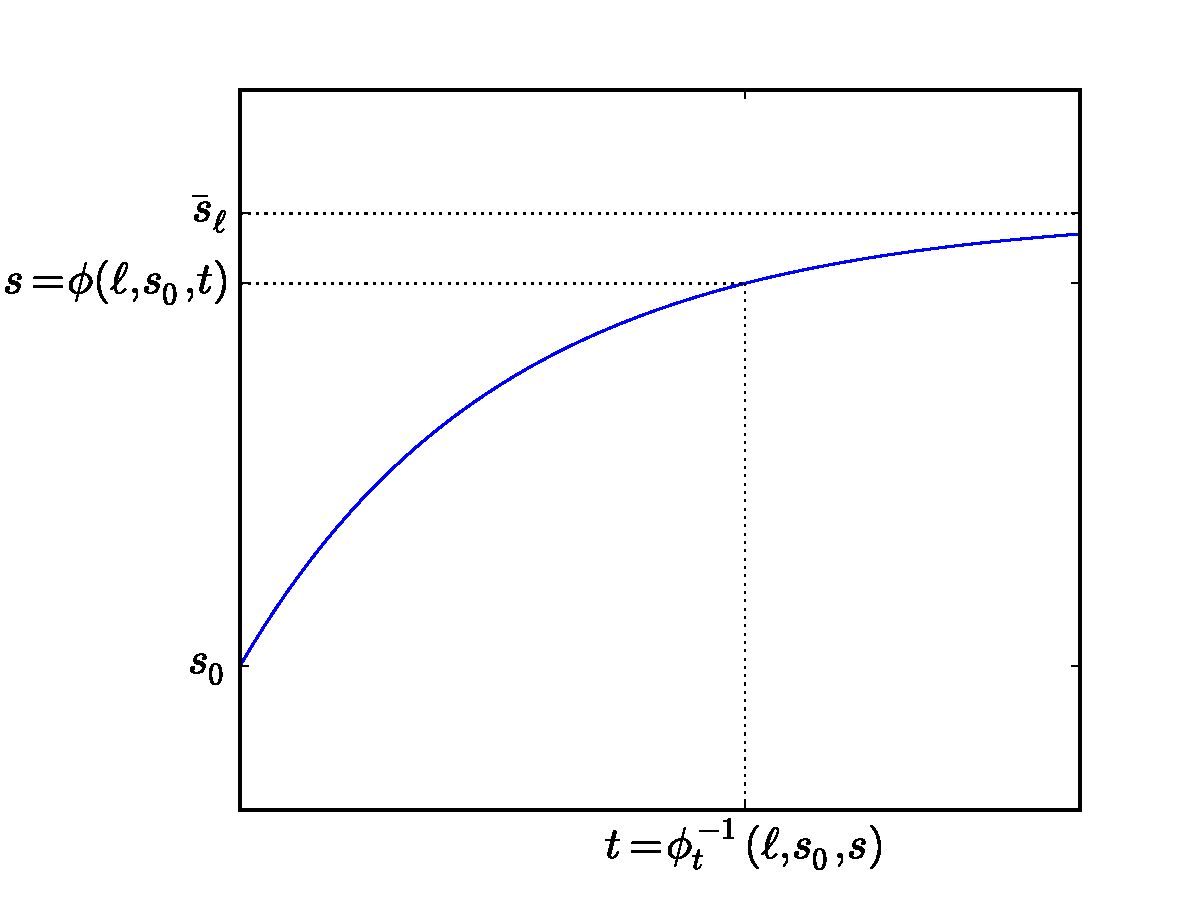
\includegraphics[height=5.5cm]{fig_flow_t}
\caption{$t\mapsto \phi(\ell,s_0,t)$}
\end{subfigure}
\begin{subfigure}{0.45\textwidth}
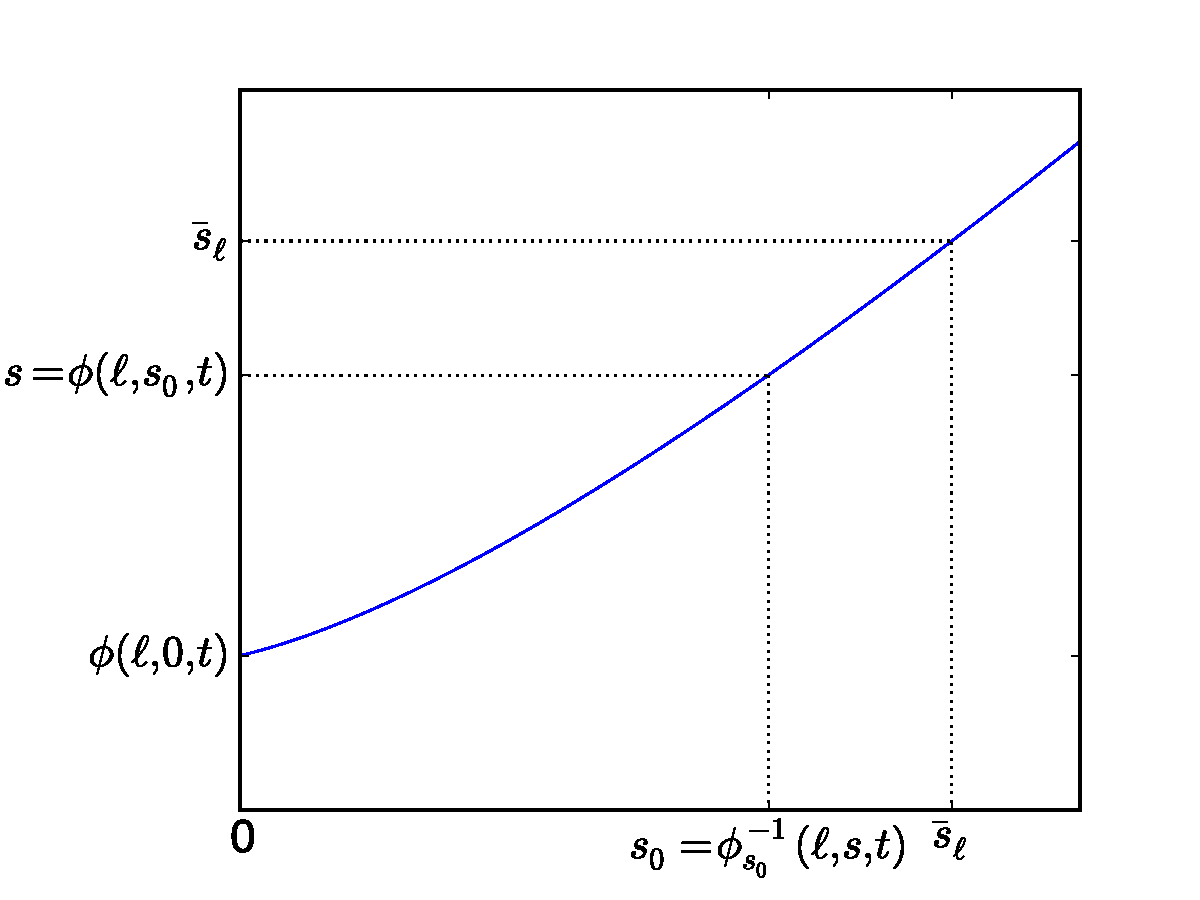
\includegraphics[height=5.5cm]{fig_flow_sO}
\caption{$s_0\mapsto \phi(\ell,s_0,t)$}
\end{subfigure}
\end{center}
\caption{\label{fig.flow}
Graphical representation of $t\mapsto \phi(\ell,s_0,t)$ and $s_0\mapsto \phi(\ell,s_0,t)$. }
\end{figure}



\subsection{Bounds on the hitting times of the process}\label{sect:irre}


In this section, we will develop some irreducibility properties of the Crump--Young process through bounds on its hitting times, which will be useful to prove the mass ratio inequality in Section~\ref{sec:mass.ratio}. To that end, let $K$ be a non empty compact set of $\NN^*\times (0,\bar s_1)$ and let $\SminK=\min_{(x, s)\,\in\,K} s $ and $\SmaxK=\max_{(x, s)\,\in\,K} s $. We will prove that each point of $K\backslash \bigcup_{\ell\,\geq\,1}(\ell,\bar s_\ell)$ can be reached, in a uniform way, from any point of $K$. Points $(\ell,\bar s_\ell)$ can not be reached.

There exists $L_{\SminK}\in\NN^*$, such that $\bar s_\ell < \SminK$ for all $\ell\geq L_{\SminK}$ (see Lemma~\ref{lem:defsbar}), let then set $\lmax=\max\{\max_{(\ell, s)\in K} \ell,\, L_{\SminK}\}$. The constants $\SminK$, $\SmaxK$ and $\lmax$ satisfy $K\subset \setunlmax\times[\SminK,\SmaxK]\subset \setunlmax\times (\bar s_{\lmax},\bar s_1)$.


Let also
\begin{align}\label{def:tmin}
t_{\min}:= \max\left\{\phit\left(1,\bar s_{\lmax},\SmaxK\right),\, \,\phit\left(\lmax,\bar s_1,\SminK\right)\right\}
\end{align}
be the maximum between the time to go from $\bar s_{\lmax}$ to $\SmaxK$ with one individual and the time to go from $\bar s_1$ to $\SminK$ with $\lmax$ individuals. Since both times are finite then $t_{\min}\linebreak<\infty$. Note that, from the monotony properties of the flow (see Lemma~\ref{lem:rapprochement}) for all $s_1,s_2$ such that $\bar s_{\lmax}\leq s_1\leq s_2\leq \SmaxK$, then $\phit(1,s_1,s_2)\leq \phit(1,\bar s_{\lmax},\SmaxK) \leq t_{\min}$ and for all $s_1,s_2$ such that $\SminK\leq s_2\leq s_1\leq \bar s_1$, $\phit(\lmax,s_1,s_2)\leq \phit(\lmax,\bar s_1,\SminK)\leq t_{\min}$. Then $t_{\min}$ is the minimal quantity such that, for all $s_1, s_2$ satisfying $\bar s_{\lmax}\leq s_1\leq s_2\leq \SmaxK$ or $\SminK\leq s_2\leq s_1\leq \bar s_1$, there exists $L\in \setunlmax$, such that $\phit(L,s_1,s_2)\leq t_{\min}$ (i.e. the substrate concentration $s_2$ is reachable from $s_1$ in a time less than $t_{\min}$ with a constant bacterial population in $\setunlmax$).


\begin{prop}\label{prop.partout.a.partout}
For all $\tau_0>t_{\min}$, $\tau>\tau_0$, $\varepsilon>0$ and $\delta>0$, there exists $C>0$, such that, for all $(x,s)\in K$, for all $(y,r)\in K$ satisfying $|r-\bar s_y|>\delta$, we have
\[
\PP_{(x,s)}\left(\tau-\varepsilon \leq \tilde T_{y,r} \leq \tau\right)\geq C>0\,,
\]
where $\tilde T_{y,r}:= \inf\{t\geq \tau_0,\, (X_t,S_t)=(y,r)\}$ is the first hitting time of $(y,r)$ after $\tau_0$.
\end{prop}

The proof of Proposition~\ref{prop.partout.a.partout} relies on a sharp decomposition of all possible combinations of initial conditions. Instead of giving all details on the proof, we will expose its main steps and the technicalities are postponed in Appendix.
\begin{proof}
Let
\begin{multline*}
\bar \varepsilon:=\\
\mkern-10mu\min\!\left\{
\frac{3\,\min\left\{\SminK-\bar s_{\lmax},\, \bar s_1-\SmaxK\right\}} {\max\left\{D\,\Sin,\, k\,\barmu\,\lmax\right\}} \,, \,
\frac{4\,\min\left\{\SminK-\bar s_{\lmax},\,\bar s_1-\SmaxK\right\}\,D\,\left(\tau_0-t_{\min}\right)/2} {\max\left\{D\,\Sin,\, k\,\barmu\,\lmax\right\}\,\left(1+D\,\left(\tau_0-t_{\min}\right)/2\right)}\!\right\}\!.
\end{multline*}
We assume, without loss of generality, that $0<\varepsilon\leq \min\{\tau-\tau_0; \bar \varepsilon\}$ because if the result holds for all $\varepsilon>0$ sufficiently small, then it holds for all $\varepsilon>0$. Assuming $0<\varepsilon\leq \frac{3\,\min\{\SminK-\bar s_{\lmax},\, \bar s_1-\SmaxK\}}{\max\{D\,\Sin,\, k\,\barmu\,\lmax\}}$ ensures that, for $(y,r)\in K$, $\bar s_{\lmax}\leq \phis(y,r,\frac{\varepsilon}{3})\leq\bar s_1$ (and consequently that $\bar s_{\lmax}\leq \phis(y,r,\frac{\varepsilon}{4})\leq\bar s_1$); see Lemma~\ref{lemme.control.phi_moins_s}-\ref{lemme.control.phi_moins_s.maj} and Remark~\ref{phis0.less.sin}. Consequently $\clS_{y,r}^\varepsilon:=\setunlmax \times [\phis(y,r,\frac{\varepsilon}{3}), \phis(y,r,\frac{\varepsilon}{4})] \subset \setunlmax \times [\bar s_{\lmax}, \bar s_1]$.



To prove Proposition~\ref{prop.partout.a.partout}, we will prove that, with positive probability, the process:
\begin{enumerate}
\item reaches the set $\clS_{y,r}^\varepsilon$ before $\tau_0$;
\item stays in this set until the time $\tau-\varepsilon$;
\item reaches $(y,r)$ in the time interval $[\tau-\varepsilon,\,\tau]$.
\end{enumerate}
These steps are illustrated in Figure~\ref{fig.proof.prop.almost.everywhere} and the associated probabilities are bounded from below in lemmas below. These ones are proved in Appendix~\ref{sec.proofs.lemmas}. To state them, let us introduce $\clE_{y,r}^\varepsilon$, defined by
\begin{multline*}
\clE_{y,r}^\varepsilon\\
:=\left\{\left(\ell,r^\varepsilon_{y,r}\right) \, \middle| \, \ell \in \setunlmax \text{ and } \bar s_\ell \geq r^\varepsilon_{y,r}\right\} \mathbin{\scalebox{1.5}{\ensuremath{\cup}}} \left\{\left(\ell,R^\varepsilon_{y,r}\right) \, \middle| \, \ell \in \setunlmax \text{ and } \bar s_\ell \leq R^\varepsilon_{y,r}\right\}\\
\subset\clS_{y,r}^\varepsilon,
\end{multline*}
where $r^\varepsilon_{y,r}= \min(\phis(y,r,\frac{\varepsilon}{3}),\phis(y,r,\frac{\varepsilon}{4}))$ and $R^\varepsilon_{y,r}=\max(\phis(y,r,\frac{\varepsilon}{3}),\phis(y,r,\frac{\varepsilon}{4}))$. The set $\clE_{y,r}^\varepsilon$ represents the points $(\ell,s) \in \clS_{y,r}^\varepsilon$ such that $s$ belongs to the bounds of the substrate part $[\phis(y,r,\frac{\varepsilon}{3}), \phis(y,r,\frac{\varepsilon}{4})]$ and $\ell$ is such that the flow $t\mapsto \phi(\ell,s,t)$ leads the dynamics to stay in $[\phis(y,r,\frac{\varepsilon}{3}), \phis(y,r,\frac{\varepsilon}{4})]$, at least for small $t$, if $\phis(y,r,\frac{\varepsilon}{3})\neq \phis(y,r,\frac{\varepsilon}{4})$ (that is if $r\neq\bar s_y$). Note that $\clE_{y,r}^\varepsilon$ is well defined if $r=\bar s_y$ and we obtain $\clE_{y,\bar s_y}^\varepsilon=\setunlmax \times \{\bar s_y\}$.


\begin{figure}
\begin{center}
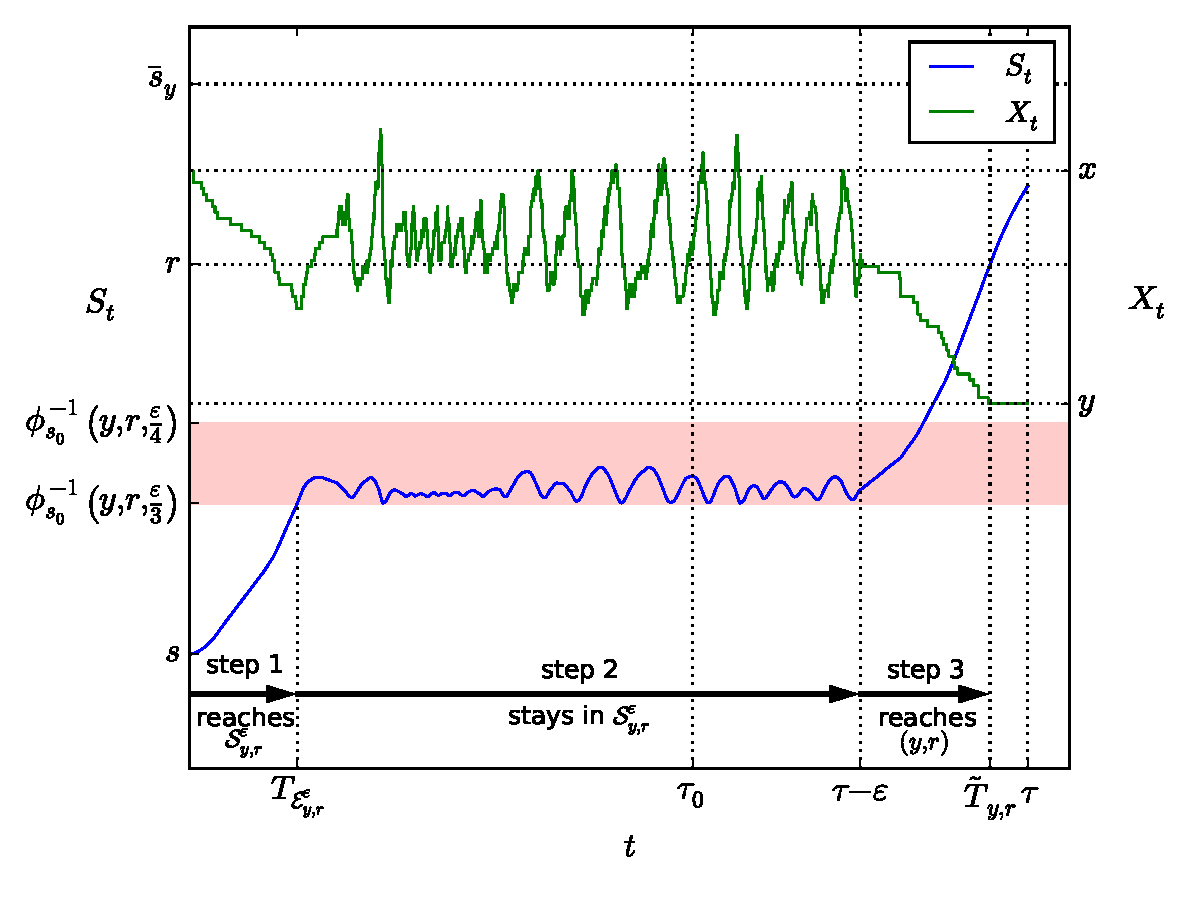
\includegraphics[width=10cm]{fig_from_xs_to_yr.pdf}
\end{center}
\caption{\label{fig.proof.prop.almost.everywhere}
Illustration of the three steps of the proof of Proposition~\ref{prop.partout.a.partout}. Step~1:~starting from $(x,s)$, the process $(X_t,S_t)_t$ reaches the set $\clS_{y,r}^\varepsilon$ before $\tau_0$. Step~2: the process stays in $\clS_{y,r}^\varepsilon$ until $\tau-\varepsilon$. Step~3: the process reaches $(y,r)$ before $\tau$. }
\end{figure}



\begin{lemm}\label{de.partout.a.presque.partout}
For all $\tau_0>t_{\min}$, there exists $C_1^{\tau_0}>0$, such that, for all $(x,s)\in K$, for all $(y,r)\in K$ and for $0<\varepsilon\leq\frac{4\,\min\{\bar s_1-\SmaxK,\, \SminK-\bar s_{\lmax}\}\,D\,(\tau_0-t_{\min})/2}{\max\{D\,\Sin,\, k\,\barmu\,\lmax\}\,(1+D\,(\tau_0-t_{\min})/2)}$,
\[
\PP_{(x,s)}\big(T_{\clE_{y,r}^\varepsilon}
\leq \tau_0\big)\geq C_1^{\tau_0},
\]
where $T_{\clE_{y,r}^\varepsilon}:=\inf\{t\geq 0,\, (X_t,S_t)\in \clE_{y,r}^\varepsilon\}$.
\end{lemm}




\begin{lemm}\label{lemma.stay.in.S}
Let $0<\varepsilon\leq \frac{3\,\min\{\SminK-\bar s_{\lmax},\, \bar s_1-\SmaxK\}}{\max\{D\,\Sin,\, k\,\barmu\,\lmax\}}$, $\delta>0$ and $T>0$. Then there exists $C^{\varepsilon,\delta,T}_2>0$, such that, for all $(y,r)\in K$ satisfying $|r-\bar s_y|>\delta$, for all $(x,s) \in \clE_{y,r}^\varepsilon$,
\[
\PP_{(x,s)}
\left((X_t,S_t) \in \clS_{y,r}^\varepsilon, \,
\forall t\in[0,T]\right)\geq C^{\varepsilon,\delta,T}_2\,.
\]
\end{lemm}




\begin{lemm}\label{lemma.Tys.depuis.S}
Let $0<\varepsilon\leq \frac{3\,\min\{\SminK-\bar s_{\lmax},\, \bar s_1-\SmaxK\}}{\max\{D\,\Sin,\, k\,\barmu\,\lmax\}}$ and $\delta>0$. Then there exists $C^{\varepsilon,\delta}_3>0$, such that, for all $(y,r)\in K$ satisfying $|r-\bar s_y|>\delta$, for all $(x,s) \in \clS_{y,r}^\varepsilon$,
\[
\PP_{(x,s)}
\Big(T_{y,r} \leq \varepsilon \Big)\geq C^{\varepsilon,\delta}_3
\]
with $T_{y,r}:=\inf\{t\geq 0, \, (X_t,S_t)=(y,r)\}$ the first hitting time of $(y,r)$.
\end{lemm}



Although not optimal, some explicit expressions of $C_1^{\tau_0}$, $C^{\varepsilon,\delta,T}_2$, $C^{\varepsilon,\delta}_3$ of the previous lemmas are obtained in Appendix~\ref{sec.proofs.lemmas}. Let us show below that they imply the conclusion of Proposition~\ref{prop.partout.a.partout}.
\begin{multline}\label{probability.decomposition}
 \PP_{(x,s)}\left(\tau-\varepsilon \leq \tilde T_{y,r} \leq \tau\right)
\\
\begin{aligned}
& \geq \PP_{(x,s)}\Big(\left\{T_{\clE_{y,r}^\varepsilon}\leq \tau_0\right\}
\cap \big\{\left(X_t,S_t\right) \in \clS_{y,r}^\varepsilon, \,
\forall t\in\left[T_{\clE_{y,r}^\varepsilon}, \, \tau-\varepsilon\right]\big\}\\
&\mkern170mu
\cap \left\{\tau-\varepsilon \leq \tilde T_{y,r} \leq \tau\right\}\Big)
\\
&\geq \PP_{(x,s)}\big(T_{\clE_{y,r}^\varepsilon}\leq \tau_0\big)\,
\times
\PP_{(x,s)}
\Big(\left(X_t,S_t\right) \in \clS_{y,r}^\varepsilon, \,
\forall t\in\left[T_{\clE_{y,r}^\varepsilon}, \, \tau-\varepsilon\right] \ \Big| \ T_{\clE_{y,r}^\varepsilon}\leq \tau_0 \Big)
\\
&\qquad
\times \PP_{(x,s)}
\Big(\tau-\varepsilon \leq \tilde T_{y,r} \leq \tau \ \Big| \ T_{\clE_{y,r}^\varepsilon}\leq \tau_0, \, \left(X_t,S_t\right) \in \clS_{y,r}^\varepsilon, \,
\forall t\in\left[T_{\clE_{y,r}^\varepsilon}, \, \tau-\varepsilon\right] \Big)\,.
\end{aligned}
\end{multline}

By Lemma~\ref{de.partout.a.presque.partout}, the first probability of the last member of~\eqref{probability.decomposition} is bounded from below by a constant $C_1^{\tau_0}>0$. By Lemma~\ref{lemma.stay.in.S} and the Markov property the second probability is bounded from below by a constant $C^{\varepsilon,\delta,\tau}_2>0$. By definition, $\tilde T_{y,r} \geq \tau_0$, moreover $(y,r) \notin \clS_{y,r}^\varepsilon$, therefore on the event

\[
\left\{\left(X_0,S_0\right)=(x,s), \, T_{\clE_{y,r}^\varepsilon}\leq \tau_0, \, \left(X_t,S_t\right) \in \clS_{y,r}^\varepsilon, \, \forall t\in\left[T_{\clE_{y,r}^\varepsilon}, \, \tau-\varepsilon\right]\right\}
\]
we have $\tilde T_{y,r}\geq \tau-\varepsilon$ almost surely. By Lemma~\ref{lemma.Tys.depuis.S} and the Markov property, the third probability is bounded from below by a constant $C^{\varepsilon,\delta}_3>0$, which achieves the proof of Proposition~\ref{prop.partout.a.partout}.
\end{proof}


\subsection{Proof of the sufficient conditions leading to Theorem~\ref{th:main-qsd}}\label{sec:QS.behavior}


We prove in this section that the three conditions -- Bounds on Lyapunov functions~\eqref{tag.BLF1} and~\eqref{tag.BLF2}; Minorization condition~\eqref{tag:SSA} and Mass ratio inequality~\eqref{tag:MRI} -- hold. Since it was proved in Section~\ref{sec:sufficient.conditions} that they imply Theorem~\ref{th:main-qsd}, it will conclude the proof of this theorem.

Bounds on Lyapunov functions~\eqref{tag.BLF1} and~\eqref{tag.BLF2} are given by Lemma~\ref{lem:lyapunov}; Minorization condition~\eqref{tag:SSA} is given by Lemma~\ref{lem:smallset}; Mass ratio inequality\eqref{tag:MRI} is given by Lemma~\ref{lem:ratio}.

\subsubsection{Bounds on Lyapunov functions}\label{sec:lyapunov}


Let $\tilde V(x,s)=V(x,s)\,\1_{(x,s)\,\in\,\NN^*\times(0,\bar s_1)}$ for all $(x,s)\in (\NN^*\times(0,\bar s_1)) \cup (\{0\}\times (0,\Sin))$, where we remind that $V$ is defined on $\NN^*\times(0,\bar s_1)$ by~\eqref{def:psi_V}. Assumptions~\eqref{hyp:theta_p} and a simple computation lead to the following lemma, whose the proof is postponed in Appendix (see Section~\ref{sec:proof.lem.LV}).

\begin{lemm}\label{lem:LV}
There exist $\eta>D$ and $\zeta>0$ such that
\[
\clL \tilde V \leq -\eta \tilde V + \zeta \psi,
\]
on $(\NN^*\times(0,\bar s_1)) \cup (\{0\}\times (0,\Sin))$, where $\clL$ is the infinitesimal generator of $(X_t,S_t)_{t\,\geq\,0}$ defined by~\eqref{eq:generator}.
\end{lemm}

Using well-known martingale properties associated to the Crump--Young model, Lemma~\ref{lem:LV} extends into the following lemma.


\begin{lemm}\label{lem:lyapunov}
There exist $\eta>D$ and $\zeta>0$, such that for all $t\geq 0$, $x\in \NN^*$ and $s\in (0,\bar s_1)$, we have
\begin{equation}\label{eq:encadrepsi}
e^{-D t}\, x = e^{-D t} \psi(x,s)
\leq \EE_{(x,s)}\left[\psi\left(X_t, S_t\right)\right]
\leq e^{\left(\mu\left(\bar s_1\right)-D\right) t}\, \psi(x,s)= e^{\left(\mu\left(\bar s_1\right)-D\right) t} \,x
\end{equation}
and
\begin{equation}\label{eq:V}
\EE_{(x,s)}\left[V\left(X_t,S_t\right) \, \1_{X_t\,\neq\,0}\right] \leq e^{-\eta t} V(x,s) + \zeta \frac{e^{\left(\mu(\bar s_1)-D\right)t}}{\eta-D} \psi(x,s)\,.
\end{equation}
\end{lemm}


\begin{proof}
It is classical (see for example~\cite[Section~4]{CF15}) that, for $f\in\clC^{0,1}(\NN\times \RR_+)$, the process
\begin{equation}\label{eq:martingale}
\left(f(X_t,S_t) - f(X_0,S_0) - \int_0^t \clL f(X_u,S_u) \dif u \right)_{t\,\geq\,0}
\end{equation}
is a local martingale. Since $\psi \leq \tilde V$ on $(\NN^*\times(0,\bar s_1)) \cup(\{0\}\times (0,\Sin))$, from Lemma~\ref{lem:LV}, $\tilde V$ satisfies $\clL\tilde V\leq \zeta \tilde V $ for some $\zeta>0$. Then using classical stopping time arguments (see~\cite[Section~6.2.]{BCGM} or~\cite[Theorem~2.1]{MTIII} and its proof for instance), we can show that it is a martingale when $f=\tilde V$ and then that $(\EE_{(x,s)}[\tilde V(X_t,S_t)])_{t\,\in\,[0,T]}$ is bounded for all $T>0$. Consequently, \eqref{eq:martingale} is also a martingale for $f=\psi$, because $\psi \leq \tilde V$. Then, from the dominated convergence theorem and the fact that, from the expression of $\psi$,
\[
-D \psi \leq \clL \psi \leq (\mu(\bar s_1) -D)\psi,
\]
we obtain~\eqref{eq:encadrepsi}. Similarly, by the linearity of $\clL$, from Lemma~\ref{lem:LV} and~\eqref{eq:encadrepsi},
\[
\clL\left(\tilde V-\frac{\zeta}{\eta-D}\psi\right)
\leq -\eta \tilde V + \zeta \psi + \frac{\zeta}{\eta-D}D\psi = -\eta\left(\tilde V-\frac{\zeta}{\eta-D}\psi\right)
\]
then, for all $(x,s)\in \NN^*\times (0,\bar s_1)$
\begin{align*}
\EE_{(x,s)}\left[V(X_t,S_t) \, \1_{X_t\neq 0}\right] &= \EE_{(x,s)}\left[\tilde V(X_t,S_t)\right]
\\
&\leq e^{-\eta\,t}\tilde V(x,s) + \frac{\zeta}{\eta-D}\left(\EE_{(x,s)}\left[\psi(X_t,S_t)\right]-e^{-\eta\,t}\psi(x,s)\right)
\\
&\leq e^{-\eta\,t} V(x,s)+\frac{\zeta}{\eta-D}\,e^{(\mu(\bar s_1)-D) t}\psi(x,s)\,.
\end{align*}
and~\eqref{eq:V} holds.
\end{proof}


This part is similar to the approach used in the proof of~\cite[Theorem~4.1]{CMMS}. In fact, in order to prove the existence of the QSD, tightness is sufficient and is ensured by the use of Lyapunov functions (see for instance~\cite[Theorem~4.2]{CMMS2011}). The significance of our work lies in proving the minorization condition~\eqref{tag:SSA} and the mass ratio inequality~\eqref{tag:MRI}, for our process, which is not irreducible and includes a deterministic component. These properties are the objectives of the next two sections.

\subsubsection{Minorization condition}\label{sec:small.set}


Let $K$ be a compact set of $\NN^*\times (0,\bar s_1)$. In agreement with the notations of Section~\ref{sect:irre}, let $s_K:=\min_{(x,s)\,\in\,K}s$ and $S_K:=\min_{(x,s)\,\in\,K}s$ be respectively the minimal and maximal substrate concentration of elements of $K$.

Our aim in this subsection is to prove the minorization condition~\eqref{tag:SSA} established page~\pageref{tag:SSA} by introducing the coupling measure $\nu$. The proof is based on Lemma~\ref{lem:bertrand} below.

\begin{lemm}\label{lem:bertrand}
Let $\tau>0$, let $0<s_0<s_K$, $s_1>s_0$ and $x\in \NN^*$. Then there exists $\epsilon_0>0$ such that, for all $(y,r)\in K$,
\[
\PP_{(y,r)}\big((X_{\tau},S_{\tau})\in \{x\}\times [s_0,s_1]\big) \geq \epsilon_0\,.
\]
\end{lemm}

Lemma~\ref{lem:bertrand} is proved in Appendix (see Section~\ref{sec:lem.bertrand}). As for Proposition~\ref{prop.partout.a.partout}, its proof relies on sharp pathwise estimates. From this, we deduce the next result which is one the cornerstone of the proof of Theorem~\ref{th:main-qsd}.

\begin{lemm}\label{lem:smallset}
For every $\tau>0$, there exist $\epsilon>0$ and a probability measure $\nu$ on $\NN^*\times (0,\bar s_1)$ such that
\begin{align}\label{eq:smallset}
\forall (y,r) \in K, \quad \PP_{(y,r)}\left((X_\tau, S_\tau) \in \cdot \right)\geq \epsilon \nu.
\end{align}
If moreover $K = \llbracket 1, N \rrbracket \times [\delta_1, \delta_2]$, for some $N \in \NN^*$ and $\delta_2>\delta_1>0$, then we can choose $\nu$ such that $\nu(K)=1$.
\end{lemm}

\begin{proof}
Starting from $(y,r) \in K$, the discrete component can reach any point $z$ of $\NN^*$ in any time interval with positive probability, so we can easily use any Dirac mass $\delta_z$ (times a constant) as a lower bound for the first marginal of the law of $(X_\tau, S_\tau)$. Let us use $z=1$. For the continuous component, we can use the randomness of the last jump time to prove that its law has a lower bound with Lebesgue density. Consequently to prove~\eqref{eq:smallset}, we consider the paths going to $\{2\} \times [s_0,s_1]$ for some $s_1\geq s_0$ well chosen, then being subjected to a washout, and we study the last jump to construct a lower bound with density.

Let us consider some $\bar s_1> s_1>s_0>0$ such that $s_0<s_K$ and $0<\tau_0<\tau$ which will be fixed at the end of the proof. On the one hand, from Lemma~\ref{lem:bertrand}, there exists $\epsilon_0>0$ such that for all $(y,r)\in K$,
\begin{equation}\label{eq:smallsetpresque0}
\PP_{(y,r)}\big((X_{\tau-\tau_0},S_{\tau-\tau_0})\in \{2\}\times [s_0,s_1]\big) \geq \epsilon_0.
\end{equation}

On the other hand, let $f$ be any positive function, $s \in [s_0,s_1]$ and $t>0$. By conditioning on the first jump time and using the Markov property, we have
\begin{multline*}
\EE_{(2,s)}\left[f(X_t,S_t)\right]
= e^{-2\,D\, t - 2\,\int_0^t \mu (\phi(2,s,u)) \dif u} \,f\left(2, \phi(2,s,t)\right)\\
\begin{aligned}
&+ \int_0^t 2\,D \,e^{-2\,D\, v - 2\,\int_0^v \mu (\phi(2,s,u)) \dif u} \,\EE_{(1,\phi(2,s,v))}\left[f(X_{t-v},S_{t-v})\right] \dif v\\
&+ \int_0^t 2\,\mu (\phi(2,s,v)) \, e^{-2\,D\,v - 2\,\int_0^v \mu (\phi(2,s,u)) \dif u} \,
\EE_{(3,\phi(2,s,v))}\left[f(X_{t-v},S_{t-v})\right] \dif v\\
&\geq \int_0^t 2\,D \, e^{-2\,D \, v - 2\,\int_0^v \mu (\phi(2,s,u)) \dif u} \times e^{-\, (t-v)\,D - \int_0^{t-v} \mu (\phi(1,\phi(2,s,v),u)) \dif u} \\
&\times f\left(1, \phi(1,\phi(2,s,v),t-v)\right) \dif v,
\end{aligned}
\end{multline*}
where the last bound comes from a second use of the Markov property on the second term. Roughly, we bounded our expectation by considering the event ``the first event is a washout and occurs during the time interval $(0,t)$ and no more jump occurs until $t$''.


Since $s\mapsto \phi(x,s,u)$ and $x\mapsto \phi(x,s,u)$ are respectively increasing and decreasing (see Lemma~\ref{prop.monotony.flow}) and $\mu$ is increasing, we have for all $s\in [s_0,s_1]$
\[
\mu (\phi(2,s,u)) \leq \mu (\phi(1,s_1,u)),
\]
hence
\begin{align*}
\EE_{(2,s)}\left[f(X_t,S_t)\right] &\geq 2\,D\, e^{-2\,D \,t} e^{ - 2\,\int_0^t \mu (\phi(1,s_1,u)) \dif u}\, \int_0^t f\left(1, \phi(1,\phi(2,s,v),t-v)\right) \dif v.
\end{align*}
By the flow property and Lemma~\ref{prop.monotony.flow}, for $0<\varepsilon < t-v$, we have
\begin{align*}
\phi(1,\phi(2,s,v),t-v) & =
\phi(1,\phi(1,\phi(2,s,v),\varepsilon),t-(v+\varepsilon))
\\
&>
\phi(1,\phi(2,\phi(2,s,v),\varepsilon),t-(v+\varepsilon))
\\
&= \phi(1,\phi(2,s,v+\varepsilon),t-(v+\varepsilon))
\end{align*}
and then $v\mapsto \phi(1,\phi(2,s,v),t-v)$ is strictly decreasing on $[0,t]$. Moreover from~\eqref{eq:flow} the derivative of $u\mapsto \phi(1,s,u)$ is bounded from above by $D\,\Sin$. Since $r\mapsto \phi(1,r,t-v)$ is increasing for $r\leq \bar s_1$ from Lemma~\ref{lem:rapprochement}, then from the expression $\phi(1,r,t-v) = r + \int_0^{t-v} (D(\Sin-\phi(1,r,u))-k\,\mu(\phi(1,r,u)))\,\dif u$, we have $0\leq\frac{\dif}{\dif r}\phi(1,r,t-v)\leq 1$. In addition, either $s\leq \bar s_2$ and $\frac{\dif}{\dif v}\phi(2,s,v)\geq 0$ or $s< \bar s_2$ and from~\eqref{eq:flow} and Lemma~\ref{lem:rapprochement}, $\frac{\dif}{\dif v}\phi(2,s,v)\geq -2\,k\,\mu(\bar s_2)$. So finally, from the chain rule formula
\begin{multline*}
\frac{\dif}{\dif v} \phi(1,\phi(2,s,v),t-v) \\= \frac{\dif}{\dif v}\phi(2,s,v)\,\frac{\dif}{\dif r} \phi(1,r,t-v)_{\vert_{r=\phi(2,s,v)}} - \frac{\dif}{\dif u} \phi(1,\phi(2,s,v),u)_{\vert_{u=t-v}},
\end{multline*}
the derivative of $v\mapsto \phi(1,\phi(2,s,v),t-v)$ is then bounded from below by $-D\,\Sin-2\,k\,\mu(\bar s_2)$. By a change of variable, for every $s_0<s_1$, we have for $c_0=[D\,\Sin+2\,k\,\mu(\bar s_2)]^{-1}$ and for $s\in (s_0,s_1)$
\begin{align*}
\EE_{(2,s)}\left[f(X_t,S_t)\right] &\geq c_{0} \,2\,D \, e^{-2\, D\, t} e^{ - 2\,\int_0^t \mu (\phi(1,s_1,u)) \dif u}\, \int_{\phi(2,s,t)}^{\phi(1,s,t)} f(1,w) \dif w \\
&\geq c_{0} \,2\, D e^{-2\, D\, t}\, e^{ - 2\,\int_0^t \mu (\phi(1,s_1,u)) \dif u} \,\int_{\phi(2,s_1,t)}^{\phi(1,s_0,t)} f(1,w) \dif w,
\end{align*}
where the last term is non negative as soon as $\phi(2,s_1,t)<\phi(1,s_0,t)$. First, we fix any $s_0<s_K$. Since $\phi(2,s_0,t)<\phi(1,s_0,t)$, by continuity, we can find $ s_1 > s_0$ satisfying $\phi(2,s_1,t)<\phi(1,s_0,t)$. Fixing such two points $s_0$ and $s_1$ for $t=\tau_0$ with $0<\tau_0<\tau$, then leads to
\begin{equation}\label{eq:smallsetpresque}
\forall s\in [s_0,s_1], \quad \PP_{(2,s)}\left((X_{\tau_0},S_{\tau_0})\in \cdot\right) \geq \epsilon_1 \nu,
\end{equation}
with
\[
\nu(dy,ds) =\delta_{1}(dy) \frac{\1_{[\phi(2,s_1,\tau_0),\phi(1,s_0,\tau_0)]} (s)}{\phi(1,s_0,\tau_0) -\phi(2,s_1,\tau_0)} ds,
\]
and
\[
\epsilon_1= c_{0} \, 2\,D \, e^{-2\,D\,\tau_0}\, e^{ - 2\,\int_0^{\tau_0}\mu (\phi(1,s_1,u)) \dif u} (\phi(1,s_0,\tau_0) -\phi(2,s_1,\tau_0)).
\]
As a consequence, from~\eqref{eq:smallsetpresque0} and~\eqref{eq:smallsetpresque}, Equation~\eqref{eq:smallset} holds with $\epsilon=\epsilon_0 \epsilon_1$, by the Markov property.


If $K = \llbracket 1, N \rrbracket \times [\delta_1, \delta_2]$, even if it means choosing $\tau_0$ small enough, $s_0$ and $s_1$ can be chosen such that they furthermore satisfy $\phi(1,s_0,\tau_0)> \delta_1$ and $\phi(2,s_1,\tau_0)< \delta_2$. Then $\nu(K)>0$ and~\eqref{eq:smallsetpresque} holds with $\tilde \epsilon_1$ and the probability measure $\tilde \nu$, satisfying $\tilde \nu(K)=1$, defined by
\[
\tilde \nu = \frac{\nu\left(\1_K\, \cdot \right)}{\nu(K)}, \qquad \tilde \epsilon_1= \epsilon_1\, \nu(K)\,.
\]
Note that if $\tau_0<\phit(2,0,\delta_2)$ (i.e. $\phis(2,\delta_2,\tau_0)>0$) then such $s_0$ and $s_1$ exist. In fact, we can choose $s_0$ and $s_1$ such that $s_0\in (\phis(1,\delta_1,\tau_0), \delta_1\wedge \phis(2,\delta_2,\tau_0))$ and $s_1\in (s_0, \phis(2,\delta_2,\tau_0)\wedge \phis(2,\phi(1,s_0,\tau_0),\tau_0))$. Since $\delta_1<\bar s_1$ and because $\ell\mapsto \phis(\ell,s,\tau_0)$ and $s\mapsto \phis(\ell,s,\tau_0)$ are both increasing (by definition of $\phis$ and by Lemma~\ref{prop.monotony.flow}), we can check that $\delta_1$ and $\delta_2$ are well defined. Moreover $s_0$ and $s_1$ are such that $s_0<\delta_1=s_K $ and $s_0<s_1$, and by Lemma~\ref{prop.monotony.flow}, we have
\begin{align*}
\phi(1,s_0,\tau_0)> \phi(1,\phis(1,\delta_1,\tau_0),\tau_0) &\geq \delta_1;
\\
\phi(2,s_1,\tau_0)<\phi(2, \phis(2,\delta_2,\tau_0), \tau_0) &=\delta_2;
\\
\phi(2,s_1,t)<\phi(2,\phis(2,\phi(1,s_0,\tau_0),\tau_0),\tau_0) &=\phi(1,s_0,\tau_0).\qedhere
\end{align*}
\end{proof}


\subsubsection{Mass ratio inequality}\label{sec:mass.ratio}

Our aim in this subsection is to prove the mass ratio inequality~\eqref{tag:MRI} given on page~\pageref{tag:MRI} by using our bounds on the hitting time given in Proposition~\ref{prop.partout.a.partout}.

\begin{lemm}\label{lem:ratio}
Let $K$ be a compact set of $\NN^*\times (0,\bar s_1)$, then
\[
\sup_{(x,s),(y,r)\,\in \,K}\; \sup_{t\,\geq\,0} \frac{\EE_{(y,r)} \left[\psi (X_{t}, S_{t})\right]}{\EE_{(x,s)} \left[\psi (X_{t}, S_{t})\right]} <+ \infty.
\]
\end{lemm}


\begin{proof}
We set $L=\max_{(x,s)\,\in\,K}x$, $\SminK=\min_{(\ell, s)\in K} s $ and $\SmaxK=\max_{(\ell, s)\,\in\,K} s $. Let
\begin{equation}\label{eq:deltadef}
0<\delta < \min\left\{\frac{1}{2} \min_{y,z \in K, \, y\neq z } |\bar s_y - \bar s_z|\, ; \, \bar s_1-\SmaxK\right\}.
\end{equation}
Note that, from Lemma~\ref{lem:defsbar}, elements of $(\bar s_\ell)_{\ell \,\in\,K}$ are all distinct and then the right member of~\eqref{eq:deltadef} is then strictly positive. Let also 
\[
\tilde K := \llbracket 1, L+1 \rrbracket \times [\min\{s_K, \bar s_L\}, \max\{S_K, \bar s_2\}]
\]
be a compact set of $\NN^*\times (0,\bar s_1)$ such that $K\subset \tilde K$ and let $t_{\min}$ defined by~\eqref{def:tmin} for the compact set $\tilde K$. Let $\tau>t_{\min}$, from~\eqref{eq:encadrepsi},
\[
\sup_{(x,s),(y,r)\,\in\,K} \sup_{t\,\leq\,\tau} \frac{\EE_{(y,r)} \left[\psi (X_{t}, S_{t})\right]}{\EE_{(x,s)} \left[\psi (X_{t}, S_{t})\right]}
\leq e^{\mu(\bar s_1)\,\tau}\,L<+ \infty,
\]
then it remains to prove that there exist $C>0$, such that for all $(x,s),(y,r) \in K$ and $t\geq \tau$, we have
\begin{align}\label{eq:ratio.t.geq.tau}
\EE_{(y,r)} \left[\psi (X_{t}, S_{t})\right]\leq C\,\EE_{(x,s)} \left[\psi (X_{t}, S_{t})\right].
\end{align}

We first show by Proposition~\ref{prop.partout.a.partout} that~\eqref{eq:ratio.t.geq.tau} holds for
\[
(y,r)\in \tilde K \setminus \left(\bigcup_{\ell= 1}^{L+1} \{\ell\} \times \clB(\bar s_\ell, \delta)\right)
\]
with $\clB(\bar s_\ell, \delta):=\{r,\, |r-\bar s_\ell|\leq\delta\}$. Then for $(y,r) \in K \cap \bigcup_{\ell= 1}^L \{\ell\} \times \clB(\bar s_\ell, \delta)$, conditioning on the first event, either no jump occurs and we make use of~\eqref{eq:encadrepsi}, or a jump occurs and the process after the jump belongs to $\tilde K \setminus(\bigcup_{\ell= 1}^{L+1} \{\ell\} \times \clB(\bar s_\ell, \delta))$ which then allows to use~\eqref{eq:ratio.t.geq.tau}.


By the Markov property, for all $0\leq u\leq t$, for all $(y,r)\in \tilde K$, $\EE_{(y,r)}[\psi(X_t,S_t)] = \EE_{(y,r)}[\EE_{(X_{t-u},S_{t-u})}[\psi(X_u,S_u)]] $. Applying~\eqref{eq:encadrepsi} to $\EE_{(X_{t-u},S_{t-u})}[\psi(X_u,S_u)]$, we then obtain
\begin{equation}\label{eq:esppsi}
\begin{split}
e^{-D\,u}\,\EE_{(y,r)}\left[\psi(X_{t-u},S_{t-u})\right]
&\leq \EE_{(y,r)}\left[\psi(X_t,S_t)\right]
\\
&\leq e^{(\barmu-D)u}\,\EE_{(y,r)}\left[\psi(X_{t-u},S_{t-u})\right].
\end{split}
\end{equation}

Mimicking the arguments of the proof of~\cite[Theorem~1.1]{CG20}, we then deduce that for every $(x,s) \in K \subset \tilde K$ and $(y,r)\in \tilde K \setminus (\bigcup_{\ell= 1}^{L+1} \{\ell\} \times \clB(\bar s_\ell, \delta))$, for all $t\geq \tau$,
\begin{equation}\label{eq:presqueA4}
\begin{split}
\EE_{(x,s)} \left[\psi \left(X_t, S_t\right)\right] &\geq \EE_{(x,s)} \left[\1_{T_{y,r} \,\leq\,\tau} \times \EE_{(y,r)}\left[\psi\left(X_{t- u}, S_{t- u}\right)\right]_{\vert_{u=T_{y,r}}}\right]\\
&\geq \PP_{(x,s)}\left(T_{y,r} \leq \tau \right) \int_0^\tau \EE_{(y,r)}\left[\psi\left(X_{t- u}, S_{t-u}\right)\right] \sigma^{x,s}_{y,r}(\dif u)\\
&\geq \tilde C\int_0^\tau e^{-(\barmu-D) u} \sigma^{x,s}_{y,r}(\dif u) \EE_{(y,r)} \left[\psi (X_t, S_t)\right]\\
&\geq \tilde C e^{-(\barmu-D) \tau} \EE_{(y,r)} \left[\psi (X_t, S_t)\right], 
\end{split}
\end{equation}
with $T_{y,r}:=\inf\{t\geq 0, \, (X_t,S_t)=(y,r)\}$ the first hitting time of $(y,r)$ and $\tilde C>0$. In the first line, we used the strong Markov property, in the second line $\sigma^{x,s}_{y,r}$ represents the law of $T_{y,r}$ conditionally to $\{((X_0,S_0)=(x,s)) \cap (T_{y,r}\leq \tau)\}$ and the third line comes from~\eqref{eq:esppsi} and Proposition~\ref{prop.partout.a.partout}.


It remains to extend the previous inequality to $(y,r) \in K \cap \bigcup_{\ell= 1}^L \{\ell\} \times \clB(\bar s_\ell, \delta)$. By conditioning on the first jump and using the Markov property, we have
\begin{multline}\label{eq:duhamel}
\EE_{(y,r)} \left[\psi (X_t, S_t)\right]= e^{-D\,y \,t - y\,\int_0^t \mu (\phi(y,r,u)) \dif u} \,\psi\left(y, \phi(y,r,t)\right)\\
\begin{aligned}
&+ \int_0^t y\,D \,e^{-D \,y \,v - y\,\int_0^v \mu (\phi(y,r,u)) \dif u}\, \EE_{(y-1, \phi(y,r,v))} \left[\psi (X_{t-v}, S_{t-v})\right] \dif v\\
&+ \int_0^t y\,\mu (\phi(y,r,v)) e^{-D\, y\, v - y\, \int_0^v \mu (\phi(y,r,u)) \dif u} \, \EE_{(y+1, \phi(y,r,v))} \left[\psi (X_{t-v}, S_{t-v})\right] \dif v.
\end{aligned}
\end{multline}
First notice that, since $\delta<\bar s_1- \SmaxK$, then ($y,r)$ necessarily satisfies $y\geq 2$. Therefore $(y-1, \phi(y,r,v))\in \tilde K$ and $(y+1, \phi(y,r,v))\in \tilde K$ (see Lemma~\ref{lem:rapprochement}).

From the definition of $\psi$ and~\eqref{eq:encadrepsi}, we have, for any $(x,s)\in K$
\begin{align}\label{eq:duhamel_term1}
\psi\left(y, \phi(y,r,t)\right) &= \frac{y}{x} \psi\left(x, s\right)
\leq \frac{y}{x}\,e^{D \,t} \, \EE_{(x,s)} \left[\psi (X_t, S_t)\right].
\end{align}
From~\eqref{eq:esppsi},
\begin{align*}
\EE_{\left(y-1, \phi(y,r,v)\right)} \left[\psi (X_{t-v}, S_{t-v})\right]
\leq & e^{D\,v}\,\EE_{\left(y-1, \phi(y,r,v)\right)} \left[\psi (X_{t}, S_{t})\right].
\end{align*}
Now since $(y, r) \in \bigcup_{\ell=1}^L \{\ell\} \times \clB(\bar s_\ell, \delta)$, then $r \in \clB(\bar s_y, \delta),$ and $\phi(y,r,v) \in \clB(\bar s_y, \delta)$ for all $v\geq 0$ because of Lemma~\ref{lem:rapprochement} (i.e. equilibrium points are attractive). Thus, by definition of $\delta$, we have
\begin{align*}
\left|\phi(y,r,v)- \bar s_{y-1} \right|
\geq \left|\bar s_{y-1}- \bar s_y \right| - \left|\phi(y,r,v) - \bar s_{y} \right| > 2\delta - \delta=\delta,
\end{align*}
then
\[
(y-1, \phi(y,r,v)) \notin \bigcup_{\ell=1}^L \{\ell\} \times\clB(\bar s_\ell, \delta).
\]
We can then apply~\eqref{eq:esppsi} and~\eqref{eq:presqueA4} to obtain
\begin{equation}\label{eq:duhamel_term2}
\begin{split}
\EE_{\left(y-1, \phi(y,r,v)\right)} \left[\psi \left(X_{t-v}, S_{t-v}\right)\right] & \leq e^{D\,v}\,\EE_{(y-1, \phi(y,r,v))} \left[\psi (X_t, S_t)\right] \\
& \leq e^{D\,v}\,\tilde C^{-1} e^{(\barmu-D) \tau} \EE_{(x,s)} \left[\psi \left(X_{t}, S_{t}\right)\right] \,.
\end{split}
\end{equation}
Similarly, we have
\begin{align}\label{eq:duhamel_term3}
\EE_{\left(y+1, \phi(y,r,v)\right)} \left[\psi \left(X_{t-v}, S_{t-v}\right)\right]
\leq & e^{D\,v}\, \tilde C^{-1} e^{(\barmu-D) \tau} \EE_{(x,s)} \left[\psi \left(X_{t}, S_{t}\right)\right] \,.
\end{align}
From~\eqref{eq:duhamel}-\eqref{eq:duhamel_term1}-\eqref{eq:duhamel_term2} and~\eqref{eq:duhamel_term3}, we then obtain
\begin{multline*}
\EE_{(y,r)} \left[\psi \left(X_t, S_t\right)\right]\\
\begin{aligned}
&\leq \EE_{(x,s)} \left[\psi \left(X_{t}, S_{t}\right)\right]\,\Big(e^{-D\,(y-1)\, t - y\,\int_0^t \mu (\phi(y,r,u)) \dif u} \frac{y}{x}\\
&\quad + \tilde C^{-1}\,e^{(\barmu-D) \tau} \,\int_0^t y\,\left(D+\mu (\phi(y,r,v))\right)\, e^{-D\,(y-1)\, v -y \,\int_0^v \mu \left(\phi(y,r,u)\right) \dif u}\, \dif v\Big)\,.
\\
&\leq \left(L\wedge \tilde C^{-1}e^{(\barmu-D) \tau}\right)\,\EE_{(x,s)} \left[\psi (X_{t}, S_{t})\right]
\\ & \qquad \times \left(1+ \,\int_0^t D\, e^{-D\,(y-1)\, v -y \,\int_0^v \mu (\phi(y,r,u)) \dif u}\, \dif v\right)\,.
\end{aligned}
\end{multline*}
Since $y\geq 2$, then
\begin{align*}
\int_0^t D\, e^{-D\,(y-1)\, v - \int_0^v y \mu (\phi(y,r,u)) \dif u}\, \dif v & \leq \int_0^t D\, e^{-D\, v} \dif v \leq 1
\end{align*}
and~\eqref{eq:ratio.t.geq.tau} holds with $C:=2\,(L\wedge \tilde C^{-1}e^{(\barmu-D) \tau})$, which finishes the proof of Lemma~\ref{lem:ratio}.
\end{proof}



\section{Proof of Corollary~\ref{co:yaglom}}\label{sec:proof.corollary}


\begin{proof}
Let us now show that the convergence towards the quasi-stationary distribution $\pi$, established in Theorem~\ref{th:main-qsd}, extends for initial measures with support larger than $\X$. The proof is in two parts, first we extend the convergence to initial conditions in $\NN^*\times (0,+\infty)$ and then for $S_0=0$.

For the first part of the proof, it is sufficient to show that $h$ can be extended for all $(x,s) \in \NN^* \times [\bar s_1,+\infty)$ such that $h(x,s)\in (0,\infty)$ and
\begin{align}\label{eq:cv.exp.lamt.exp}
\lim_{t\,\to\,\infty} e^{\lambda t} \EE_{(x,s)} [f(X_t,S_t)] = \pi(f) \times h(x,s),
\end{align}
for any bounded function on $\NN \times \RR_+$ such that $f(0,\cdot) =0$. In fact, if such function $h$ exists, then choosing $f(x,s)=\1_{x\,\neq\,0}$ leads to $h(x,s)= \lim_{t\,\to\,\infty} e^{\lambda t}\PP_{(x,s)} (\Text>t)$ (extending the definition of $h$ given by~\eqref{def:h} on $\NN^* \times \RR_+$) and the result holds.

Let $\epsilon>0$ and set $T_\epsilon=T_{ \NN^*\times (0,\bar s_1-\epsilon]}$ being the hitting time of $\NN^*\times (0,\bar s_1-\epsilon]$. We have
\begin{align*}
\EE_{(x,s)} \left[f(X_t,S_t)\right] &= \EE_{(x,s)} \left[f(X_t,S_t)\1_{\left(T_\epsilon\,\wedge\,\Text\right)\,\leq\,t}\right] + \EE_{(x,s)} \left[f(X_t,S_t)\1_{\left(T_\epsilon\,\wedge \,\Text\right)\,>\,t}\right].
\end{align*}

On the one hand, from Lemma~\ref{lem:lyap2} we can choose $\epsilon$ sufficiently small such that, from the Markov inequality,
\begin{align}\label{eq:proba.T_epsilon}
\PP_{(x,s)}\left(T_\epsilon\wedge \Text >t\right)\leq \EE_{(x,s)}\left[e^{(D+C)\left(T_\epsilon\,\wedge\,\Text\right)} \right] e^{-(D+C)t} \leq A e^{\beta s} e^{-(D+C)t},
\end{align}
where $A$, $\beta$ and $C$ are positive constants (which depend on $\epsilon$) given by Lemma~\ref{lem:lyap2}. Since $\lambda \leq D$ by~\eqref{eq:eigenvalue.bounds}, we then have
\begin{align*}
e^{\lambda t}\EE_{(x,s)}\left[f(X_t,S_t)\1_{T_\epsilon\,\wedge\,\Text\,>\,t}\right] &\leq \|f \|_\infty e^{\lambda t} \PP_{(x,s)}\left(T_\epsilon\wedge \Text>t\right) \\
&\leq \|f \|_\infty A e^{\beta s} e^{-Ct} \longrightarrow_{t\,\to\,\infty} 0\,.
\end{align*}
On the other hand, noting that $f(X_t,S_t)\1_{\Text\,\leq\,t}=0$, from the strong Markov Property
\begin{multline}\label{eq:T_eps_leq_t}
e^{\lambda t}\EE_{(x,s)} \left[f(X_t,S_t)\1_{(T_\epsilon\,\wedge\,\Text)\,\leq\,t}\right]
\\
\begin{aligned}
&=e^{\lambda t}\EE_{(x,s)} \left[f(X_t,S_t)\1_{T_\epsilon\,\leq\,t}\right] \\
&= e^{\lambda t} \EE_{(x,s)} \left[
\EE_{\left(X_{T_\epsilon},S_{T_\epsilon}\right)}\left[f(X_{u},S_{u}) \right]_{\vert_{u=t-T_\epsilon}} \1_{T_\epsilon\,\leq\,t} \right].
\end{aligned}
\end{multline}
Moreover, fixing $\rho>1$ and $p\in(0,\frac{\mu(\bar s_1)-D}{D+k\,\mu'(\bar s_1)})$, for all $0<\tilde \omega\leq \omega$ (with $\omega$ depending on $\rho$ and $p$), since~\eqref{eq:cv_qsd_X_eq_h} holds replacing $\omega$ by $\tilde \omega$ and as, by continuity of the process $(S_t)_t$, $(X_{T_\epsilon},S_{T_\epsilon})\in\NN^*\times \{\bar s_1-\epsilon\}\subset \NN^*\times (0,\bar s_1)$ on the event $\{T_\epsilon\leq t\}$, we obtain
\begin{multline}\label{eq:cv.T_eps_leq_t}
 \left|e^{\lambda t}\,\EE_{(x,s)} \left[
\EE_{\left(X_{T_\epsilon},S_{T_\epsilon}\right)}\left[f\left(X_{u},S_{u}\right) \right]_{\vert_{u=t-T_\epsilon}} \1_{T_\epsilon\,\leq\,t} \right]\right.\\
-\left. \EE_{(x,s)} \left[e^{\lambda T_\epsilon} \, h\left(X_{T_\epsilon},S_{T_\epsilon}\right)\pi(f) \1_{T_\epsilon\,\leq\,t} \right] \right|\\
\begin{aligned}
&\leq
\EE_{(x,s)} \left[e^{\lambda T_\epsilon} \left| e^{\lambda(t-T_\epsilon)}
\EE_{\left(X_{T_\epsilon},S_{T_\epsilon}\right)}\left[f\left(X_{u},S_{u}\right) \right]_{\vert_{u=t-T_\epsilon}}-h\left(X_{T_\epsilon},S_{T_\epsilon}\right)\pi(f)\right| \1_{T_\epsilon\,\leq\,t} \right]\\
&\leq \|f\|_\infty\,C\,e^{-\tilde\omega\,t}
\EE_{(x,s)} \left[e^{\left(\lambda+\tilde\omega\right)\,T_\epsilon}W_{\rho,p}\left(X_{T_\epsilon},S_{T_\epsilon}\right) \1_{T_\epsilon\,\leq\,t} \right].
\end{aligned}
\end{multline}
In addition,
\begin{align*}
\EE_{(x,s)} \left[e^{\left(\lambda+\tilde \omega\right)\, T_\epsilon}W_{\rho,p}\left(X_{T_\epsilon},S_{T_\epsilon}\right) \1_{T_\epsilon\,\leq\,t} \right] &\leq
\tilde C\, \EE_{(x,s)} \left[e^{\left(\lambda+\tilde\omega\right)\, T_\epsilon} \,V_0\left(X_{T_\epsilon},S_{T_\epsilon}\right) \, \1_{T_\epsilon\,\leq\,t} \right]
\end{align*}
with $\tilde C=\log(\rho)\,e^{-\alpha(\bar s_1-\varepsilon)}+(\bar s_1-\epsilon)^{-1}+\epsilon^{-p}$ and $V_0$ defined by $V_0(x,s)=\rho^{x}\,e^{\alpha\,s}/\log(\rho)$ for all $(x,s)\in \NN\times \RR_+$. In the same way as in Section~\ref{sec:proof.lem.LV}, for all $\eta>0$, there exists $C_\eta>0$ such that $\clL(V_0(x,s)-C_\eta)\leq -\eta (V_0(x,s) - C_\eta)$ for all $(x,s)\in \NN^*\times \RR_+$. And by the same arguments used in the proof of Lemma~\ref{lem:lyap2}, $((V_0(X_t,S_t)-C_\eta)\,e^{\eta\,t})_t$ is a submartingale. Then by the stopping time theorem and remarking that $\{T_\epsilon\leq t\} \subset \{T_\epsilon\leq \Text\}$, we obtain for $\eta=\lambda+\tilde \omega$
\begin{multline}\label{eq:dom.exp.T_eps.V_0}
\EE_{(x,s)} \left[e^{(\lambda+\tilde\omega)\, T_\epsilon}W_{\rho,p}\left(X_{T_\epsilon},S_{T_\epsilon}\right) \1_{T_\epsilon\,\leq\,t} \right]
\\
\begin{aligned} 
&\leq
\tilde C\, \left|\EE_{(x,s)} \left[e^{\left(\lambda+\tilde\omega\right)\, T_\epsilon\,\wedge\,t} \,\left(V_0\left(X_{T_\epsilon\,\wedge\,t},S_{T_\epsilon\,\wedge\,t}\right)-C_\eta\right)\right]\right| +\tilde C\,C_\eta\, \EE_{(x,s)} \left[e^{\left(\lambda+\tilde\omega\right)\, T_\epsilon}\1_{T_\epsilon\,\leq\,t} \right]
\\ 
&\leq \tilde C\,\left|V_0(x,s)-C_\eta\right| +\tilde C\,C_\eta\, \EE_{(x,s)} \left[e^{\left(\lambda+\tilde\omega\right)\, \left(T_\epsilon\,\wedge \,\Text\right)} \right]\,.
\end{aligned}
\end{multline}
By~\eqref{eq:eigenvalue.bounds}, $\lambda \leq D$. Then, for $0<\tilde \omega\leq \omega$ sufficiently small (smaller than the constant $C$ of Lemma~\ref{lem:lyap2}), Lemma~\ref{lem:lyap2} and~\eqref{eq:dom.exp.T_eps.V_0} lead to
\begin{align}\label{eq:esp.W.bounded}
\EE_{(x,s)} \left[e^{\left(\lambda+\tilde\omega\right)\, T_\epsilon}W_{\rho,p}\left(X_{T_\epsilon},S_{T_\epsilon}\right) \1_{T_\epsilon\,\leq\,t} \right]
\leq \tilde C\,\left|V_0(x,s)-C_\eta\right| +\tilde C\,C_\eta\, A\,e^{\beta\,s}\,.
\end{align}
Hence, \eqref{eq:T_eps_leq_t}, \eqref{eq:cv.T_eps_leq_t} and~\eqref{eq:esp.W.bounded} gives
\begin{align*}
e^{\lambda t}\EE_{(x,s)} \left[f(X_t,S_t)\1_{\left(T_\epsilon\wedge \Text\right)\,\leq\,t}\right]
\longrightarrow_{t\,\to\,\infty} \pi(f) \,\EE_{(x,s)} \left[e^{\lambda T_\epsilon} h\left(X_{T_\epsilon},S_{T_\epsilon}\right) \1_{T_\epsilon\,<\,\infty}\right],
\end{align*}
where we used that $h\leq C_h\, W_{\rho,p}$ on $\NN^*\times (0,\bar s_1)$, \eqref{eq:esp.W.bounded} and the dominated convergence theorem. Then, \eqref{eq:cv.exp.lamt.exp} holds with $h(x,s)=\EE_{(x,s)} [e^{\lambda T_\epsilon} h(X_{T_\epsilon},S_{T_\epsilon}) \1_{T_\epsilon < \infty}]$ for all $(x,s) \in \NN^* \times [\bar s_1,+\infty)$, which is finite by the previous arguments. Moreover Lemma~\ref{lem:lyap2} ensures that $h(x,s)>0$.



It remains to show the result for $s=0$. Let $x\in \NN^*$, the Markov property gives for $t'>t>0$,
\begin{align*}
\EE_{(x,0)} \left[f(X_{t'},S_{t'}) \ \middle| \ \Text>t'\right] &=\frac{\EE_{(x,0)} \left[f\left(X_{t'},S_{t'}\right) \1_{\Text\,>\,t'} \right]}{\EE_{(x,0)} \left[\1_{\Text\,>\,t'}\right]}\\
& =\frac{\EE_{(x,0)} \left[f(X_{t'},S_{t'}) \1_{\Text\,>\,t'} \ | \ \Text> t \right]}{\EE_{(x,0)} \left[\1_{\Text>t'} \ | \ \Text> t\right]}\\
&=\frac{\EE_{(x,0)} \left[\EE_{\left(X_{t},S_{t}\right)}\left[f\left(X_{t'-t},S_{t'-t}\right) \1_{\Text>(t'-t)} \right] \ \middle| \ \Text> t \right]}{\EE_{(x,0)} \left[\EE_{(X_{t},S_{t})}\left[\1_{\Text>t'-t} \right] \ \middle| \ \Text> t \right]}\\
&=\frac{\EE_{\xi} \left[f\left(X_{t'-t},S_{t'-t}\right) \1_{\Text\,>\,(t'-t)} \right]}{\EE_{\xi} \left[\1_{\Text\,>\,t'-t} \right] }\\
&=\EE_{\xi} \left[f(X_{t'-t},S_{t'-t}) \ \middle| \ \Text>(t'-t) \right]\\
\end{align*}
where $\xi$ is the law of $(X_{t},S_{t})$ conditioned on the event $\{ \Text> t \}\cap\{(X_0,S_0)=(x,0)\}$. Assume that $\xi$ is a probability distribution on $\NN^*\times (0,\bar s_1)$, then, from~\eqref{eq:cv_qsd},
\begin{multline*}
\sup_{\|f \|_\infty\,\leq\,1 } \left|\EE_{\xi} \left[f(X_{t'-t},S_{t'-t}) \ \middle| \ \Text>t'-t\right] - \pi(f) \right| \\
\leq C \min\left(\frac{\xi\left(W_{\rho,p}\right)}{\xi(h)}, \frac{\xi\left(W_{\rho,p}\right)}{\xi(\psi)}\right) e^{-\omega (t'-t)}
\end{multline*}
with $\rho>1$ and $p\in(0,\frac{\mu(\bar s_1)-D}{D+k\,\mu'(\bar s_1)})$. Since $\xi(\psi)\neq 0$ (or $\xi(h)\neq 0$ because from Theorem~\ref{th:main-qsd}, $h(y,r)\in(0,\infty)$ for all $(y,r)\in\NN^*\times (0,\bar s_1)$), then Corollary~\ref{co:yaglom} holds for $s=0$ if in addition $\xi(W_{\rho,p})=\EE_{(x,0)}[W_{\rho,p}(X_t,S_t) \ | \ \Text> t]<+\infty$. So let us prove that, for $\rho$ sufficiently small, $\xi$ is a probability distribution on $\NN^*\times (0,\bar s_1)$ and that $\xi(W_{\rho,p})<+\infty$, which both consist of proving that
\[
\EE_{(x,0)}\left[\frac{1}{S_t} \ \middle| \ \Text >t\right] <+\infty.
\]
Indeed, note that conditionally on the non-extinction $S_t\leq \phi(1,0,t)< \bar s_1$. Moreover $(X_t)_t$ can be stochastically dominated by a pure birth process with birth rate $\mu(\bar s_1)$, whose the law at time $t$ is a negative binomial distribution with parameters $x$ and $e^{- \mu(\bar s_1) t}$. Then, for $1<\rho<(1-e^{\mu(\bar s_1)t})^{-1}$, $\EE_{(x,0)}[\rho^{X_t} \ | \ \Text >t]\leq (e^{- \mu(\bar s_1) t}\,\rho /(1- \rho\,(1-e^{- \mu(\bar s_1) t})))^x$.


Since the process $(X_t)_t$ dominates a pure death process with death rate (\emph{per capita}) $D$, we have $\PP_{(x,0)}(\Text > t) \geq e^{-D x t}$, then it is sufficient to prove that for all (sufficiently small) $t>0$,

\[
\EE_{(x,0)}\left[\frac{1}{S_t} \right] <+\infty.
\]
Instead of using a Lyapunov function, we prove this bound using a coupling method. On $[0,t]$, from~\eqref{eq:substrate} and given that $S_0=0$, we have the following upper-bound
\[
\forall u\in [0,t], \quad S_u \leq (S_0 + D\Sin t)\wedge \Sin \leq D\Sin t,
\]
and also the two following ones
\[
\forall s\in[0,D\Sin t], \quad \mu(s) \leq \bar\mu_t, \ \mu'(s) \leq \bar\mu'_t,
\]
for some constant $\bar\mu_t, \bar\mu'_t>0$. Consequently, we can couple $(X_u)_{u\,\in\,[0,t]}$ with a Yule process $(Z_u)_{u\,\in \,[0,t]}$ (namely a pure birth process) with jumps rate (\emph{per capita}) $\bar\mu_t$ in such a way
\[
\forall u\leq t, \quad X_u \leq Z_u.
\]
In particular, $X_u\leq Z_t$. From this bound and the evolution equation of the substrate~\eqref{eq:substrate}, we have
\begin{align}\label{eq:min.S}
\forall u\in [0,t], \quad S_u' \geq D(\Sin -S_u) - k \bar\mu'_t S_u Z_t,
\end{align}
and then, by a Gronwall type argument,
\[
\forall u\in [0,t], \quad S_u \geq \frac{D \Sin}{D+ k \bar\mu'_t Z_t } \left(1-e^{-D u- k \bar\mu'_t Z_t u}\right) \geq \frac{D \Sin}{D+ k \bar\mu'_tZ_t } \left(1-e^{-D u}\right).
\]
Finally using the classical equality for pure birth processes $\EE_{(x,0)}[Z_t] = x e^{\bar\mu_t t}$, we obtain
\[
\EE_{(x,0)}\left[\frac{1}{S_t} \right] \leq \frac{D+ k \bar\mu'_t x e^{\bar\mu_t t} }{D \Sin \left(1-e^{-D t}\right)},
\]
which ends the proof of Corollary~\ref{sec:proof.corollary}.
\end{proof}

Note that relaxing the assumptions as in Remark~\ref{remark:mu.lipschitz}, even if it means choosing $t$ small enough, $\bar{\mu}'_t$ can be replaced by a local Lipschitz constant in a neighborhood of $0$ in~\eqref{eq:min.S}.



\appendix



\section{Classical and simple results on the Crump--Young process}



In the present section, we gather some basic properties of the Crump--Young process, under Assumption~\ref{hyp:mu}.



\subsection{Preliminary results on the flow}\label{sec.preliminary.flow}


In this subsection, we expose simple results on the flow functions relative to the substrate dynamics with no evolution of the bacteria. We begin by results on the behavior of $\phi$, defined by~\eqref{eq:flow}, and then we give bounds on $\phit$ and $\phis$.

\begin{lemm}\label{prop.monotony.flow}
The flow satisfies the following properties: for all $s,\, \tilde s \in \RR_+$, $t> 0$, $\ell, \tilde \ell \in \NN^*$ such that $s< \tilde s$ and $\ell < \tilde \ell$
\begin{enumerate}
\item\label{lemmA.1} $\phi(\ell,s,t)>\phi(\tilde \ell,s,t)$ ;
\item\label{lemmA.2} $\phi(\ell,s,t)< \phi(\ell,\tilde s,t)$.
\end{enumerate}
\end{lemm}
\begin{proof}
The first inequality comes from the decreasing property of $\ell \mapsto D(\Sin-s)\linebreak-k\,\mu(s)\,\ell$. The second point comes from the Cauchy--Lipschitz (or Picard--Lindel\"of) theorem.
\end{proof}

\begin{lemm}\label{lem:defsbar}
For every $\ell\in \NN^*$, Equation~\eqref{eq:defsbar}, that is
\[
D(\Sin-\bar s_\ell)-k\,\mu(\bar s_\ell)\,\ell = 0\,,
\]
admits a unique solution in $(0,\Sin)$. Furthermore the sequence $(\bar s_\ell)_{\ell\,\geq\,1}$ is strictly decreasing and $\lim_{\ell\,\to\,\infty} \bar s_\ell = 0$.
\end{lemm}
\begin{proof}
The map $g_\ell:s\mapsto D(\Sin-s)-k\,\mu(s)\,\ell$ is strictly decreasing, $g_\ell(0)=D \Sin>0$, $g_\ell(\Sin)=-k\,\mu(\Sin)\ell<0$ then~\eqref{eq:defsbar} admits a unique solution in $(0,\Sin)$. Moreover, for every $s> 0$, the sequence $(g_\ell(s))_{\ell\,\geq\,1}$ is strictly decreasing then $(\bar s_\ell)_{\ell\,\geq\,1}$ is also strictly decreasing and
\[
\lim_{\ell\,\to\,\infty} \mu(\bar s_\ell) = \lim_{\ell\,\to\,\infty} \frac{D\,(\Sin-\bar s_\ell)}{k\,\ell} = 0
\]
then, by Assumption~\ref{hyp:mu}, $\lim_{\ell\,\to\,\infty} \bar s_\ell = 0$.
\end{proof}


\begin{lemm}\label{lem:rapprochement}
For every $s \in \RR_+$, $\ell \in \NN^*$ and $t\geq 0$,
\begin{enumerate}
\item\label{lemmA.3.1} if $s< \bar s_\ell$, then $u\mapsto \phi(\ell,s,u)$ is strictly increasing from $\RR_+$ to $[s,\bar s_\ell)$;
\item\label{lemmA.3.2} if $s> \bar s_\ell$, then $u\mapsto \phi(\ell,s,u)$ is strictly decreasing from $\RR_+$ to $(\bar s_\ell,s]$.
\end{enumerate}
In particular
\[
|s - \bar s_\ell| \geq \left|\phi(\ell,s,t) - \bar s_\ell \right|.
\]
\end{lemm}
\begin{proof}
By Lemma~\ref{prop.monotony.flow}, if $s< \bar s_\ell$ then $\phi(\ell,s,t) < \bar s_\ell$ for every $t\geq 0$. On $[0, \bar s_\ell)$, $\partial_t \phi(\ell,\cdot,t)$ is strictly positive because, by Assumption~\ref{hyp:mu}, $g_\ell:s\mapsto D(\Sin-s)-k\,\mu(s)\,\ell$ is strictly decreasing and $g_\ell(\bar s_\ell)=0$. Finally,
\[
s \leq \phi(\ell,s,t) < \bar s_\ell.
\]
In the same way, on $(\bar s_\ell,+\infty)$, $\partial_t \phi(\ell,\cdot,t)$ is strictly negative and $s \geq \phi(\ell,s,t) > \bar s_\ell$ for $s\geq \bar s_\ell$ which ends the proof.
\end{proof}


\begin{coro}\label{cor:monotonyphit}
For every $s_0,s_1,s_2 \in \RR_+$ and $\ell \in \NN^*$ satisfying $s_0 \geq s_1 \geq s_2 > \bar s_\ell$ or $s_0 \leq s_1 \leq s_2 < \bar s_\ell$ then
\[
\phit(\ell,s_0,s_2) = \phit(\ell,s_0,s_1)+\phit(\ell,s_1,s_2)<+\infty \,.
\]
\end{coro}
\begin{proof}
The result directly comes from the monotony properties of the flow given by Lemma~\ref{lem:rapprochement} and the flow property.
\end{proof}


\begin{lemm}\label{lem:phispos}
For all $\ell \in \NN^*$, $s\geq 0$, and $t\geq \widetilde{t}\geq 0$,
\[
\phis(\ell,s,t)>0 \Rightarrow \phis\left(\ell,s,\widetilde{t}\right)>0.
\]
\end{lemm}
\begin{proof}
On the one hand, for every $u\geq 0$, by Lemma~\ref{prop.monotony.flow} and definition of $\phis$, we have
\[
\phis(\ell,s,u)>0 \Leftrightarrow s> \phi(\ell,0,u).
\]
From Lemma~\ref{lem:rapprochement} $u \mapsto \phi(\ell,0,u)$ is increasing. Thus
\[
\phis(\ell,s,t)>0 \Leftrightarrow s> \phi(\ell,0,t) \Rightarrow s> \phi\left(\ell,0,\widetilde{t}\right) \Leftrightarrow \phis\left(\ell,s,\widetilde{t}\right)>0. \qedhere
\]
\end{proof}
\begin{lemm}\label{lemme.control.phi_moins_1}
For $\ell \in \NN^*$, $(s_0,s)\in [0,\bar s_1]^2$, such that $s_0\neq \bar s_\ell$ and $\phit(\ell,s_0,s)\linebreak<\infty$,
\[
\frac{|s-s_0|}{\max\left\{D\,\Sin,\,k\,\barmu\,\ell\right\}} \leq \phit(\ell,s_0,s) \leq \frac{|s-s_0|}{D\,|\bar s_\ell-s|}\,.
\]
\end{lemm}
\begin{proof}
Since $\phit(\ell,s_0,s)<\infty$, then
\begin{align*}
s &= s_0 + \int_0^{\phit(\ell,s_0,s)}\big[D(\Sin-\phi(\ell,s_0,u))-k\,\mu(\phi(\ell,s_0,u))\,\ell\big]\,\dif u
\\
&= s_0 + \int_0^{\phit(\ell,s_0,s)}\big[D(\bar s_\ell-\phi(\ell,s_0,u))+k\,\left(\mu(\bar s_\ell)-\mu(\phi(\ell,s_0,u))\right)\,\ell\big]\,\dif u\,.
\end{align*}
The first equality will allow to obtain the lower bound and the second one will lead to the upper bound for $\phit(\ell,s_0,s)$. Either $s_0\leq s < \bar s_\ell$ then, from Lemma~\ref{lem:rapprochement}, the flow $u \mapsto \phi(\ell,s_0,u)$ is increasing and for all $u\in[0,\,\phit(\ell,s_0,s)]$, $s_0\leq \phi(\ell,s_0,u) \leq s < \bar s_\ell$. Since $\mu$ is increasing, we then obtain,
\begin{align*}
\phit(\ell,s_0,s)\,D(\bar s_\ell-s)
\leq s-s_0 \leq \phit(\ell,s_0,s)\,D\,\Sin\,.
\end{align*}
Or $s_0 \geq s> \bar s_\ell$ then the flow $u \mapsto \phi(\ell,s_0,u)$ is decreasing and $s_0\geq \phi(\ell,s_0,u) \geq s > \bar s_\ell$ for all $u\in[0,\,\phit(\ell,s_0,s)]$. Since $\phi(\ell,s_0,u)\leq \bar s_1\leq \Sin$ and $\mu$ is increasing, we then obtain
\begin{align*}
- \phit(\ell,s_0,s)\,k\,\barmu\,\ell
\leq s-s_0 \leq \phit(\ell,s_0,s)\,D\,(\bar s_\ell-s)
\end{align*}
and the result holds.
\end{proof}




\begin{lemm}\label{lemme.control.phi_moins_s}\leavevmode
\begin{enumerate}
\item \label{lemme.control.phi_moins_s.maj}
For all $(\ell,s,\varepsilon)\in \NN^* \times [0,\bar s_1]\times \RR_+$ such that $\phis(\ell,s,\varepsilon)\leq \bar s_1$,
\[
\left|s-\phis(\ell,s,\varepsilon)\right| \leq \varepsilon \max\left\{D\,\Sin,\,k\,\barmu\,\ell\right\}\,.
\]
\item \label{lemme.control.phi_moins_s.min}
For all $(\ell,s,\varepsilon)\in \NN^* \times \RR_+\times \RR_+$ such that $\phis(\ell,s,\varepsilon)>0$,
\[
D|s-\bar s_\ell|\,\varepsilon \leq \left|s-\phis(\ell,s,\varepsilon)\right|\,.
\]
\end{enumerate}
\end{lemm}


\begin{rema}\label{phis0.less.sin}
If $s\leq \bar s_1$, then assumption $\phis(\ell,s,\varepsilon)\leq \bar s_1$ is satisfied when $\varepsilon\leq \frac{\bar s_1-s}{k\,\barmu\,\ell}$. Indeed, from Lemmas~\ref{lem:rapprochement} and~\ref{lem:defsbar}, $u\mapsto \phi(\ell,\bar s_1,u)$ is decreasing, then for all $u\geq 0$, $\phi(\ell,\bar s_1,u)\leq \bar s_1$ and
\begin{align*}
\phi(\ell,\bar s_1,\varepsilon) = \bar s_1 + \int_0^\varepsilon \big[D\left(\Sin-\phi(\ell,\bar s_1, u)\right)-k\,\mu\left(\phi(\ell,\bar s_1, u)\right)\,\ell\big]\,\dif u
\geq \bar s_1-\varepsilon\,k\,\barmu\,\ell\,.
\end{align*}
Then $\varepsilon\leq \frac{\bar s_1-s}{k\,\barmu\,\ell}$ implies that $s\leq \phi(\ell,\bar s_1,\varepsilon)$. Hence, either $\phis(\ell,s,\varepsilon)=0\leq \bar s_1$, or $\phi(\ell,\phis(\ell,s,\varepsilon),\varepsilon) = s \leq \phi(\ell,\bar s_1,\varepsilon)$ and then, by Lemma~\ref{prop.monotony.flow}, $\phis(\ell,s,\varepsilon)\leq \bar s_1$.
\end{rema}


\begin{proof}[Proof of Lemma~\ref{lemme.control.phi_moins_s}]
First, we assume that $\phis(\ell,s,\varepsilon)>0$. By definition of $\phis$,
\begin{align*}
s & = \phis(\ell,s,\varepsilon) \\
&+ \int_0^{\varepsilon}\left[D\left(\Sin-\phi\left(\ell,\phis(\ell,s,\varepsilon), u\right)\right)-k\,\mu\left(\phi\left(\ell,\phis(\ell,s,\varepsilon), u\right)\right)\,\ell\right]\,\dif u\\
& = \phis(\ell,s,\varepsilon)\\
&\; + \int_0^{\varepsilon}\left[D\left(\bar s_\ell-\phi\left(\ell,\phis(\ell,s,\varepsilon), u\right)\right)+k\,\left(\mu(\bar s_\ell)-\mu\left(\phi\left(\ell,\phis(\ell,s,\varepsilon), u\right)\right)\,\ell\right)\right]\,\dif u\,.
\end{align*}
On the one hand, if $s\leq \bar s_\ell$, then for all $u\in [0,\varepsilon]$, $\phis(\ell,s,\varepsilon)\leq \phi(\ell,\phis(\ell,s,\varepsilon), u) \leq s \leq \bar s_\ell$, hence, from the second equality and since $\mu$ is increasing,
\[
s-\phis(\ell,s,\varepsilon) \geq D(\bar s_\ell-s)\,\varepsilon>0\,.
\]
In the same way, if $s\geq \bar s_\ell$, then for all $u\in [0,\varepsilon]$, $\phis(\ell,s,\varepsilon)\geq \phi(\ell,\phis(\ell,s,\varepsilon), u) \geq s \geq \bar s_\ell$, hence
\[
\phis(\ell,s,\varepsilon) - s \geq D(s-\bar s_\ell)\,\varepsilon>0
\]
and the lower bound of $|s-\phis(\ell,s,\varepsilon)|$ then holds.

On the other hand, if $s \in [0,\bar s_1]$ and $\phis(\ell,s,\varepsilon) \in [0,\bar s_1]$, then for all $u\in[0,\varepsilon]$, $\phi(\ell,\phis(\ell,s,\varepsilon), u)\leq \bar s_1$ and from the first equality,
\[
\left|s-\phis(\ell,s,\varepsilon)\right| \leq \varepsilon \max\left\{D\,\Sin,\,k\,\barmu\,\ell\right\}\,,
\]
then the upper bound for $|s-\phis(\ell,s,\varepsilon)|$ holds for $0<\phis(\ell,s,\varepsilon)\leq \bar s_1$.

If $\phis(\ell,s,\varepsilon)=0$, then $s\leq \phi(\ell,0,\varepsilon)$ and
\begin{align*}
\left|s-\phis(\ell,s,\varepsilon)\right| =s & \leq \int_0^{\varepsilon}\big[D(\Sin-\phi(\ell,0,u))-k\,\mu(\phi(\ell,0,u))\,\ell\big]\,\dif u
\leq \varepsilon D\,\Sin
\end{align*}
and the upper bound for $|s-\phis(\ell,s,\varepsilon)| $ also holds for $\phis(\ell,s,\varepsilon)=0$.
\end{proof}



\subsection{Preliminary results on the jumps}\label{sec:preliminary.jumps}


In contrast with the previous section, in the present one, we let the bacteria evolve. Let $(T_i)_{i \in \NN^*}$ be the sequence of the jump times of the process $(X_t)_{t\geq 0}$:
\begin{align*}
T_i :=
\begin{cases}
\inf\{t> 0, \, X_{t-}\neq X_t\} & \text{if $i=1$};\\
\inf\{t>T_{ i-1}, \, X_{t-}\neq X_t\}& \text{if $i>1$.}
\end{cases}
\end{align*}

Let us also introduce a classical notation in the study of piecewise deterministic Markov process (see~\cite{BLMZ15} for instance). Let $(x_0,s_0)\in \NN^*\times \RR^+$, $0\leq t_1\leq \dots \leq t_{N+1}$ and let $\Psi\left(x_0,s_0,(t_j,x_j)_{1\,\leq\,j\,\leq\,N},t_{N+1}\right)$ be the iterative solution of
\begin{align}\label{eq:defPsi}
\left\{
\begin{matrix*}[l]
\Psi(x_0,s_0,t_1) = \phi(x_0,s_0,t_1), \\
\Psi\left(x_0,s_0,(t_j,x_j)_{1\leq j\leq i},t_{i+1}\right)
= \phi\Big(x_i,\Psi\left(x_0,s_0,(t_j,x_j)_{1\leq j\leq i-1},t_i\right), t_{i+1}-t_i\Big).
\end{matrix*}
\right.
\end{align}
Then $\Psi(x_0,s_0,(t_j,x_j)_{1\,\leq \,j\,\leq\,N},t)$ represents the substrate concentration at time $t$, given the initial condition is $(x_0,s_0)$ and that the bacterial population jumps from $x_{i-1}$ to $x_i$ at time $t_i$ for $i=1,\cdots,N$.


For all $n\in\NN^*$, $u_1,\,\dots u_n>0$, let set
\[
\clE_D(u_1,\,\dots,\,u_n):=\bigcap_{i=1}^{n}\{X_{u_i}=X_0 -i\} \cap \{T_i=u_i\}
\]
and
\[
\clE_B(u_1,\,\dots,\,u_n):=\bigcap_{i=1}^{n}\{X_{u_i}=X_0 +i\} \cap \{T_i=u_i\}
\]
the event ``the first $n$ events are washouts (respectively divisions) and occur at time $u_1,\,\dots u_n$''.


In Lemma~\ref{prop.minore.proba.evt} below, we use Poisson random measures to bound the probability of one event by the probability of this event conditionally on having followed a certain path (no jump, successive washouts or successive divisions).

\begin{lemm}\label{prop.minore.proba.evt}
Let $A$ be a measurable set (of the underlying probability space). We have the following inequalities.
\begin{enumerate}
\item\label{lemmA.9.1} For all $\delta \geq 0$ and $(x,s) \in \NN^*\times \RR_+$
\[
\PP_{(x,s)}(A)\geq \PP_{(x,s)}(A \cap \{T_1 > \delta\}) \geq e^{-(D+\mu(\bar s_1 \vee s))\,x\,\delta}\,\PP_{(x,s)}\left(A \ \middle| \ T_1 > \delta\right)\,.
\]
\item\label{lemmA.9.2} For all $\delta \geq 0$, $(x,s) \in \NN^*\times \RR_+$ and $1\leq n\leq x$,
\begin{align*}
\PP_{(x,s)}(A) & \geq
\PP_{(x,s)}
\Big(A \cap
\bigcap_{i=1}^{n}\Big\{\{T_i\ \leq\delta\} \cap \{ X_{T_i} = x-i \}\Big\}\Big)
\\
&\geq \int_0^{\delta} \int_{u_1}^{\delta}\dots \int_{u_{n-1}}^{\delta}
\left(\prod_{k=x-n+1}^{x}D\,k\right)\, e^{-(D+\mu(\bar s_1 \vee s))\,\left(x\,u_1+
\sum\limits_{i=1}^{n-1}(x-i)\,(u_{i+1}-u_{i})\right)}\,
\\
& \qquad \times
\PP_{(x,s)}
\Big(A \ \Big| \clE_D(u_1,\dots,u_n) \Big)\,
\dif u_{n}\dots\,\dif u_1\,.
\end{align*}

\item\label{lemmA.9.3} For all $\delta \geq 0$, $(x,s) \in \NN^*\times \RR_+$ and all $n\geq 1$
\begin{align*}
\PP_{(x,s)}(A) &
\geq \PP_{(x,s)}
\Big(A \cap
\bigcap_{i=1}^{n}\Big\{\{T_i\ \leq\delta\} \cap \{ X_{T_i} = x+i \}\Big\}\Big)
\\
&\geq \int_0^{\delta} \int_{u_1}^{\delta}\dots \int_{u_{n-1}}^{\delta}
\left(\prod_{k=1}^{n}\mu\left(\Psi(x,s,(u_i,x+i)_{1\,\leq\,i\,\leq\,k-1},u_k)\right)\,(x+k-1)\right)\,
\\
& \hspace{1cm} \times e^{-(D+\mu(\bar s_1 \vee s))\,\left(x\,u_1+
\sum\limits_{i=1}^{n-1}(x+i)\,\left(u_{i+1}-u_{i}\right)\right)}\,
\\
& \qquad \times
\PP_{(x,s)}
\Big(A \ \Big| \clE_B(u_1,\,\dots,\,u_n) \Big)\,
\dif u_{n}\dots\,\dif u_1\,.
\end{align*}
\end{enumerate}
\end{lemm}

\begin{proof}
Under the event $\{X_t\geq 1\}$ (or equivalently under the event $\{X_u\geq 1 \text{ for } u \in [0, t]\}$ since $\{0\}$ is an absorbing state for the process $(X_t)_t$), from the comparison theorem and Lemma~\ref{lem:rapprochement}, for all $0\leq u \leq t$ we have $S_u \leq \phi(1,S_0,u)\leq S_0\vee \bar s_1$. Let $(x,s) \in \NN^*\times \RR_+$, the individual jump rate $\mu(S_t)$ of the process $(X_t,S_t)$ starting from $(x,s)$ is then bounded by $\mu(\bar s_1\vee s)$.


The bounds established in the lemma are classical and based on the construction of the process $(X_t,S_t)$ from Poisson random measures: we consider two independent Poisson random measures $\clN _d(\dif u, \dif j, \dif \theta)$ and $\clN _w(\dif u, \dif j)$ defined on $\RR_+ \times \NN^* \times [0,1]$ and $\RR_+ \times \NN^*$ respectively, corresponding to the division and washout mechanisms respectively, with respective intensity measures
\begin{align*}
n_d(\dif u, \dif j, \dif \theta) &=
\mu(\bar s_1 \vee s) \, \dif u \, \left(\sum_{\ell\,\geq\,1} \delta_{\ell}(\dif j) \right)
\, \dif \theta\\
\intertext{and}
n_w(\dif u, \dif j) &= D \, \dif u \, \left(\sum_{\ell\,\geq\,1} \delta_{\ell}(\dif j) \right)\,.
\end{align*}
Then the process $(X_t,S_t)$ starting from $(X_0,S_0)=(x,s)$ can be defined by
\begin{multline*}
(X_t,S_t) = (x, \phi(x,s,t))\\
\begin{aligned}
&+ \int_0^t \int_{\NN^*} \int_0^1 \1_{\left\{j\,\leq\,X_{\umoins}\right\}}\,\1_{\left\{0\,\leq\,\theta \,\leq\,\mu(S_u)/\mu(\bar s_1 \vee s)\right\}}\,\\
& \qquad \quad
\left[(1, \phi(X_\umoins +1, S_u, t-u)- \phi(X_\umoins, S_u, t-u)\right]\,\clN _d(\dif u, \dif j, \dif \theta)
\\
&+ \int_0^t \int_{\NN^*} \1_{\left\{j\,\leq\,X_{\umoins}\right\}}\,
\left[(-1, \phi(X_\umoins -1, S_u, t-u)- \phi(X_\umoins, S_u, t-u)\right]\,\clN _w(\dif u, \dif j)\,.
\end{aligned}
\end{multline*}
We refer to~\cite{CF15} for more details on this construction.

\eqref{lemmA.9.1} By construction of the process, if $(X_0,S_0)=(x,s)$, we get $T_1 = T_{d}\wedge T_{w}\,$ where, $T_{d}$ is the time of the first jump of the process
\[
t\mapsto \clN _{d}\left([0,t]\times \{x\}\times \left[0,\frac{\mu(\phi(x,s,u))}{\mu(\bar s_1 \vee s)}\right] \right)
\]
and $T_{w}$ is the time of the first jump of the process $t\mapsto \clN _{w}([0,t]\times \{x\})$.

The distribution of $T_{d}$ is a non-homogeneous exponential distribution with parameter $\mu(\phi(x,s,u))\,x$, i.e. with the probability density function
\[
t\mapsto \mu(\phi(x,s,t))\,x\,\exp\left({-\int_0^t \mu(\phi(x,s,u))\,x \dif u}\right).
\]
The distribution of $T_{w}$ is a (homogeneous) exponential distribution with parameter $D\,x$. $T_{d}$ and $T_{w}$ are independent, then
\[
\PP_{(x,s)}(T_1 > \delta) = e^{-\int_0^\delta (\mu(\phi(x,s,u))+D)\,x \, \dif u}
\geq e^{-(D+\mu(\bar s_1 \vee s))\,x\,\delta}
\]
and the first result holds.


\eqref{lemmA.9.2} On the event $\bigcap_{i=1}^{k}\{\{T_i\ =u_i\} \cap \{ X_{T_i} = x-i \}\}$, the distribution of $T_{k+1}-u_k$ is a non-homogeneous exponential distribution with parameter $(\mu(\phi(x-k,S_{T_k},t))+D)\,(x-k)$ with $S_{T_k} = \Psi(x,s,(u_i,x-i)_{1\,\leq\,i \,\leq\,k-1}, u_k) \in (0,\bar s_1 \vee s)$, i.e. with the probability density function (evaluated in $t$)
\begin{multline*}
(\mu(\phi(x-k,S_{T_k},t))+D)\,(x-k)\,e^{-\int_0^t \left(\mu\left(\phi(x-k,S_{T_k},u)\right)+D\right)\,(x-k) \dif u}
\\ \qquad \geq (\mu(\phi(x-k,S_{T_k},t))+D)\,(x-k)\,e^{-(\mu(\bar s_1 \vee s)+D)\,(x-k)\,t}
\end{multline*}
and on the event $\{T_{k+1}=u\}$, the event is a bacterial washout with probability $D/(\mu(\phi(x-k,S_{T_k},u))+D)$. We then obtain the second assertion.

\eqref{lemmA.9.3} The third assertion is obtained in the same way as the second one.
\end{proof}



\section{Proofs of technical Lemmas}\label{sec.proofs.lemmas}



\subsection{Additional notation}\label{sec.add.notation.app}

For all $n\geq \ell\geq 1$ and all $t\geq0$, let $P_d(n,\ell,t)$ defined by
\begin{multline*}
P_d(n,\ell,t) = \\
\int_0^{t} \int_{u_1}^{t}\dots \int_{u_{\ell-1}}^{t}
\left(\prod_{k=n-\ell+1}^{n}D\,k\right)\, e^{-(D+\barmu)\,\left(n\,u_1+
\sum\limits_{i=1}^{\ell-1}(n-i)\,(u_{i+1}-u_{i})\right)}\,
\dif u_\ell \dots\,\dif u_1
\end{multline*}
be the probability that the $\ell$ first events are deaths and occur in the time interval $[0,t]$ for a birth-death process, with \emph{per capita} birth rate $\barmu$ and death rate $D$, starting from $n$ individuals.

For all $n\geq \ell\geq 1$ and all $t\geq0$, let $P_b(n,\ell,t)$ defined by
\begin{multline*}
P_b(n,\ell,t) =\\
\int_0^{t} \int_{u_1}^{t}\dots \int_{u_{\ell-1}}^{t}
\left(\prod_{k=n}^{n+\ell-1}\barmu\,k\right)\, e^{-(D+\barmu)\,\left(n\,u_1+
\sum\limits_{i=1}^{\ell-1}(n+i)\,(u_{i+1}-u_{i})\right)}\,
\dif u_\ell \dots\,\dif u_1
\end{multline*}
be the probability that the $\ell$ first events are births and occur in the time interval $[0,t]$ for a birth-death process, with \emph{per capita} birth rate $\barmu$ and death rate $D$, starting from $n$ individuals.


\begin{rema}\label{rk.Pd.Pb.inc}
Both maps $t\mapsto P_d(n,\ell,t)$ and $t\mapsto P_b(n,\ell,t)$ are increasing.
\end{rema}

For all $L\in\NN^*$, $\Smin,\, \Smax$ such that $\bar s_L<\Smin \leq \Smax<\bar s_1$, we define the hitting time $T_{L,[\Smin,\Smax]}$ by
\[
T_{L,[\Smin,\Smax]}:=\inf\left\{t\geq 0,\, (X_t,S_t)\in B(L,[\Smin,\Smax])\right\}\,,
\]
where
\[
B(L,[\Smin,\Smax]):=\big\{(\ell,\Smin) \, | \, \ell \in \llbracket 1,L \rrbracket \text{ and } \bar s_\ell \geq \Smin\big\} \cup 
\big\{(\ell,\Smax) \, \big| \, \ell \in \llbracket 1,L \rrbracket \text{ and } \bar s_\ell \leq \Smax\big\}\,.
\]
In addition of being a hitting time of $\llbracket 1, L \rrbracket \times [\Smin,\Smax]$, the boundary $B(L,[\Smin,\Smax])$ is chosen such that the process remains in this set during some positive time after $T_{L,[\Smin,\Smax]}$ if $\Smin<\Smax$. If $\Smin=\Smax$ then $B(L,[\Smin,\Smax])=\llbracket 1,L \rrbracket \times \{\Smin\}$.



\subsection{Proof of Lemma~\ref{de.partout.a.presque.partout}}\label{sec:partout.a.partout}


Lemma~\ref{de.partout.a.presque.partout} is a consequence of Lemma~\ref{lemma.reach.T.Smin.Smax} below.



\begin{lemm}\label{lemma.reach.T.Smin.Smax}
Let $L \in \NN^*$, $\Smin,\Smax$ such that $\bar s_L<\Smin\leq\Smax<\bar s_1$, and let $(x,s)\in \llbracket 1, L\rrbracket \times [\bar s_L,\bar s_1]$,
\begin{enumerate}
\item \label{lemma.reach.T.Smin.Smax.s_inf_Smin}
if $s\leq \Smin$, then for $\tau_0>\phit(1, s,\Smin)$,
\begin{align*}
\PP_{(x,s)}\left(T_{L,[\Smin,\Smax]}\leq \tau_0\right) &\geq e^{-(D+\barmu)\,(\tau_0-\delta)}\,P_d(x,x-1,\delta)\\
&\geq e^{-(D+\barmu)\,(\tau_0-\delta)}\,P_d(L,L-1,\delta)
\end{align*}
with $\delta:=(\tau_0-\phit\left(1, s,\Smin\right))\,\frac{D\,|\bar s_1-s|}{D\,|\bar s_1-s|+\max\{D\,\Sin,\,k\,\barmu\,L\}}$;

\item \label{lemma.reach.T.Smin.Smax.s_sup_Smax}
if $s\geq\Smax$, then for $\tau_0>\phit(L, s,\Smax)$,
\begin{align*}
\PP_{(x,s)}\left(T_{L,[\Smin,\Smax]}\leq \tau_0\right) &\geq e^{-(D+\barmu)\,(\tau_0-\delta)\,L}\,\left(\mu(\bar s_L)/\barmu\right)^{L-x}\, P_b(x,L-x, \delta)
\\
&\geq e^{-(D+\barmu)\,(\tau_0-\delta)\,L}\,
\left(\mu(\bar s_L)/\barmu\right)^{L-1}\,P_b(1,L-1, \delta)
\end{align*}
with $\delta:=(\tau_0-\phit(L, s,\Smax))\,\frac{D\,|\bar s_L-s|}{D\,|\bar s_L-s|+\max\{D\,\Sin,\,k\,\barmu\,L\}}$;

\item \label{lemma.reach.T.Smin.Smax.s_in_Smin_Smax}
if $s\in (\Smin,\Smax)$, then for $\tau_0>\phit(1, s,\Smax) \wedge \phit(L, s,\Smin)=:t^\star$
\begin{align*}
\PP_{(x,s)}\left(T_{L,[\Smin,\Smax]}\leq \tau_0\right) &\geq e^{-(D+\barmu)\,\left(\tau_0-\delta_1-\delta_2\right)\,L}\\
& \quad\times(\mu(\bar s_L)/\barmu)^{L-1}\,P_d(L,L-1, \delta_1)\, P_b(1,L-1, \delta_2)
\end{align*}
with 
\begin{align*}
\delta_1 &{:=}\frac{\tau_0-t^\star}{2}\,\frac{D\,|\bar s_1-s|}{D\,|\bar s_1-s|+\max\{D\,\Sin,\,k\,\barmu\,L\}}\\
\intertext{and}
\delta_2 &{:=}\frac{\tau_0-t^\star}{2}\,\frac{D\,|\bar s_L-s|}{D\,|\bar s_L-s|+\max\{D\,\Sin,\,k\,\barmu\,L\}}.
\end{align*}
\end{enumerate}
\end{lemm}


\begin{proof}[Proof of Lemma~\ref{de.partout.a.presque.partout}]
Let $(y,r)\in K$ and let us define $\Smin:=\phis(y,r,\frac{\varepsilon}{3})$,\linebreak $\Smax:=\phis(y,r,\frac{\varepsilon}{4})$ if $r\leq \bar s_y$ and $\Smax:= \phis(y,r,\frac{\varepsilon}{3})$, $\Smin:= \phis(y,r,\frac{\varepsilon}{4})$ if $r\geq \bar s_y$. Then $T_{\clE_{y,r}^\varepsilon}=T_{\lmax,[\Smin,\Smax]}$. From Lemma~\ref{lemme.control.phi_moins_s}-\ref{lemme.control.phi_moins_s.maj} and Remark~\ref{phis0.less.sin}, we have $|r-\phis(y,r,\frac{\varepsilon}{4})|\leq \frac{\varepsilon}{4}\,\max\{D\,\Sin,k\,\barmu y\}$, then the condition
\[
\varepsilon\leq\frac{4\,\min\left\{\bar s_1-\SmaxK,\, \SminK-\bar s_{\lmax}\right\}\,D\,(\tau_0-t_{\min})/2}{\max\left\{D\,\Sin,\, k\,\barmu\,\lmax\right\}\,\left(1+D\,(\tau_0-t_{\min})/2\right)}
\]
implies that, for $r\in [\SminK,\SmaxK]\subset [\bar s_\lmax,\bar s_1]$ and $y\in \setunlmax$,
\begin{align}\label{encadre.eps4}
\texttt{s} &\leq \phis\left(y,r,\frac{\varepsilon}{4}\right)
\leq \clS
\end{align}
with $\texttt{s}:=\SminK-\frac{(\SminK-\bar s_{\lmax})\,D\,(\tau_0-t_{\min})/2}{1+D\,(\tau_0-t_{\min})/2}$ and $\clS:= \SmaxK+\frac{(\bar s_1-\SmaxK)\,D\,(\tau_0-t_{\min})/2}{1+D\,(\tau_0-t_{\min})/2}$.\\

In addition, since $\bar s_{\lmax}\!<\!\texttt{s}\!\leq\!\SminK\!\leq\!\SmaxK\!\leq\!\clS\!<\!\bar s_1$, from Corollary~\ref{cor:monotonyphit} and Lemma \ref{lemme.control.phi_moins_1},
\begin{equation}\label{time.to.go.up}
\begin{split}
\phit\left(1,\SminK,\clS\right) &=
\phit\left(1,\SminK,\SmaxK\right) +
\phit\left(1,\SmaxK,\clS\right)\\
&\leq t_{\min} +
\frac{\clS-\SmaxK}{D\,|\bar s_1-\clS|} 
= \tau_0 -
\frac{\tau_0-t_{\min}}{2}
\end{split}
\end{equation}
and
\begin{equation}\label{time.to.go.down}
\begin{split}
\phit\left(\lmax,\SmaxK,\texttt{s}\right)&=
\phit\left(\lmax,\SmaxK,\SminK\right) +
\phit\left(\lmax,\SminK,\texttt{s}\right)\\
 &\leq t_{\min} +\frac{\SminK-\texttt{s}}{D\,|\texttt{s}-\bar s_\lmax|} = \tau_0 -
\frac{\tau_0-t_{\min}}{2}\,.
\end{split}
\end{equation}
Let set 
\begin{align*}
\delta_1 &{:=}\frac{\tau_0-t_{\min}}{2}\,\frac{D\,|\bar s_1-s|}{D\,|\bar s_1-s|+\max\{D\,\Sin,\,k\,\barmu\,\lmax\}}\\
\intertext{and}
\delta_2 &{:=}\frac{\tau_0-t_{\min}}{2}\,\,\frac{D\,|\bar s_\lmax-s|}{D\,|\bar s_\lmax-s|+\max\left\{D\,\Sin,\,k\,\barmu\,\lmax\right\}}.
\end{align*}
From~\eqref{encadre.eps4} $\Smin$ or $\Smax$ (or both) belongs to $[\texttt{s}, \clS]$, hence for $(x,s)\in K$, we have three cases.
\begin{enumerate}
\item If $s\leq \Smin$, then $\Smin \leq \clS$, from Corollary~\ref{cor:monotonyphit} and from~\eqref{time.to.go.up}
\[
\tau_0-\phit\left(1,s,\Smin\right)
\geq \tau_0 - \phit\left(1,\SminK,\clS\right)
\geq \frac{\tau_0-t_{\min}}{2} >0
\]
then from Lemma~\ref{lemma.reach.T.Smin.Smax}-\ref{lemma.reach.T.Smin.Smax.s_inf_Smin} and Remark~\ref{rk.Pd.Pb.inc},
\[
\PP_{(x,s)}\big(T_{\clE_{y,r}^\varepsilon}
\leq \tau_0\big)\geq e^{-(D+\barmu)\,(\tau_0-\delta_1)}\,P_d(\lmax,\lmax-1,\delta_1)\,;
\]

\item If $s\geq \Smax$, then $\Smax \geq \texttt{s}$, from Corollary~\ref{cor:monotonyphit} and~\eqref{time.to.go.down},
\[
\tau_0-\phit\left(\lmax,s,\Smax\right)
\geq \tau_0-\phit\left(\lmax,\SmaxK,\texttt{s}\right)
\geq\frac{\tau_0-t_{\min}}{2}>0
\]
then from Lemma~\ref{lemma.reach.T.Smin.Smax}-\ref{lemma.reach.T.Smin.Smax.s_sup_Smax} and Remark~\ref{rk.Pd.Pb.inc},
\[
\PP_{(x,s)}\big(T_{\clE_{y,r}^\varepsilon}
\leq \tau_0\big)\geq e^{-(D+\barmu)\,(\tau_0-\delta_2)\,\lmax}\,
\left(\frac{\mu(\bar s_{\lmax})}{\barmu}\right)^{\lmax-1}\,P_b(1,\lmax-1, \delta_2)\,;
\]

\item If $s\in (\Smin, \Smax)$, then $\Smin$ or $\Smax$ belongs to $[\texttt{s},\clS]$, and at least one of both conditions $\tau_0-\phit\left(1,s,\Smin\right)
\geq \frac{\tau_0-t_{\min}}{2} >0 $ or $
\tau_0-\phit\left(\lmax,s,\Smax\right)
\geq\frac{\tau_0-t_{\min}}{2}>0 $ is satisfied. We then deduce from Lemma~\ref{lemma.reach.T.Smin.Smax}-\ref{lemma.reach.T.Smin.Smax.s_in_Smin_Smax} and Remark~\ref{rk.Pd.Pb.inc} that
\begin{align*}
\PP_{(x,s)}\big(T_{\clE_{y,r}^\varepsilon}\leq \tau_0\big) &\geq e^{-(D+\barmu)\,\left(\tau_0-\frac{\delta_1+\delta_2}{2}\right)\,\lmax}\, P_d\left(\lmax,\lmax-1, \frac{\delta_1}{2}\right)\,
\\
&\qquad \times
\left(\frac{\mu(\bar s_{\lmax})}{\barmu}\right)^{\lmax-1}\,P_b\left(1,\lmax-1, \frac{\delta_2}{2}\right)\,.
\end{align*}
\end{enumerate}
Finally Lemma~\ref{de.partout.a.presque.partout} holds with
\begin{align*}
C_1^{\tau_0}&:= e^{-(D+\barmu)\,(\tau_0-\min\{\delta_1,\delta_2\})\,\lmax}\\
& \qquad
\times P_d\left(\lmax,\lmax-1, \frac{\delta_1}{2}\right)\,
\left(\frac{\mu(\bar s_{\lmax})}{\barmu}\right)^{\lmax-1}\,P_b\left(1,\lmax-1, \frac{\delta_2}{2}\right)\,.
\qedhere
\end{align*}
\end{proof}


\begin{proof}[Proof of Lemma~\ref{lemma.reach.T.Smin.Smax}]\leavevmode
\begin{proof}[{Proof of Item~\eqref{lemma.reach.T.Smin.Smax.s_inf_Smin}}]
If $s \leq \Smin$, we will prove that one way for the process to reach $B(L,[\Smin,\Smax])$ before $\tau_0$ is if the population jumps from $x$ to 1 by $x-1$ successive washout events during the time duration
\[
\delta:=(\tau_0-\phit(1, s,\Smin))\,\frac{D\,|\bar s_1-s|}{D\,|\bar s_1-s|+\max\left\{D\,\Sin,\,k\,\barmu\,L\right\}}
\]
and if then no event occurs during the time duration $\tau_0-\delta$. The main arguments of the proof are the following: we will see that during the time duration $\delta$, the substrate concentration remains greater than or equal to $s-\delta\,\max\{D\,\Sin,\,k\,\barmu\,L\}$ and that $\delta$ is chosen such that
\[
\phit\big(1, s-\delta\,\max\{D\,\Sin,\,k\,\barmu\,L\},\Smin\big)\leq \tau_0-\delta
\]
that is the remaining time after the successive washout events is enough for the substrate process to reach $\Smin$.
\begin{itemize}
\item if $x=1$ and $s_0 \in [s-\delta\,\max\{D\,\Sin,\,k\,\barmu\,L\}, \Smin]$, from Lemma~\ref{prop.minore.proba.evt} we have
\begin{align*}
\PP_{(1,s_0)}\left(T_{L,[\Smin,\Smax]}\leq \tau_0-\delta\right) & \geq
\PP_{(1,s_0)}\left(\left\{T_{L,[\Smin,\Smax]}\leq \tau_0-\delta)\right\}
\cap \left\{T_1\ > \tau_0-\delta\right\}\right)
\\
&\geq e^{-(D+\barmu)\, (\tau_0-\delta)}\,
\PP_{(1,s_0)}
\left(T_{L,\left[\Smin,\Smax\right]}\leq \tau_0-\delta \, \middle| \, T_1> \tau_0-\delta\right).
\end{align*}
Moreover, from Lemma~\ref{lemme.control.phi_moins_1}
\begin{align*}
\phit \Big(1,s-\delta\,\max\left\{D\,\Sin,\,k\,\barmu\,L\right\},s\Big) &\leq \frac{\delta\,\max\left\{D\,\Sin,\,k\,\barmu\,L\right\}}{D\,|\bar s_1-s|} =T
\end{align*}
with $T=(\tau_0-\phit(1, s,\Smin))\,\frac{\max\{D\,\Sin,\,k\,\barmu\,L\}}{D\,|\bar s_1-s|+\max\{D\,\Sin,\,k\,\barmu\,L\}}$. Then from Corollary~\ref{cor:monotonyphit},
\begin{align*}
\phit\left(1, s_0,\Smin \right) &= \phit \Big(1,s-\delta\,\max\left\{D\,\Sin,\,k\,\barmu\,L\right\},\Smin\Big)
\\ &\quad- \phit \Big(1,s-\delta\,\max\left\{D\,\Sin,\,k\,\barmu\,L\right\},s_0\Big)
\\
&\leq \phit \Big(1,s-\delta\,\max\left\{D\,\Sin,\,k\,\barmu\,L\right\},s\Big)+\phit \Big(1,s,\Smin\Big)
\\
&\leq T+\phit \Big(1,s,\Smin\Big) = \tau_0 - \delta\,.
\end{align*}
Then, since from Lemma~\ref{lem:rapprochement} $t\mapsto \phi(1, s_0,t)$ is increasing,
\begin{align*}
\phi(1,s_0,\tau_0-\delta) &\geq \phi\left(1,s_0,\phit\left(1, s_0,\Smin \right)\right)=\Smin\,.
\end{align*}
On the event $\{(X_0,S_0)=(1,s_0), \, T_1> \tau_0-\delta \}$, we then have $S_{\tau_0-\delta} \geq \Smin$ a.s. Since $(S_t)_{t\,\geq\,0}$ is a continuous process, from the intermediate value theorem, $(S_t)_{t\,\geq \,0}$ reaches $\Smin$ in the time interval $[0,\tau_0-\delta]$. Moreover, since $\Smin<\bar s_1$ then
\[
\PP_{(1,s_0)}
\left(T_{L,[\Smin,\Smax]}\leq \tau_0-\delta \, \middle| \, T_1> \tau_0-\delta\right)=1
\]
and therefore
\begin{align}\label{eq.reach.Smin.Smax.befor.tmax.x1}
\PP_{(1,s_0)}\left(T_{L,[\Smin,\Smax]}\leq \tau_0-\delta \right) &\geq e^{-(D+\barmu)\,(\tau_0-\delta)}\,.
\end{align}
Since $\PP_{(1,s)}(T_{L,[\Smin,\Smax]}\leq \tau_0) \geq \PP_{(1,s)}(T_{L,[\Smin,\Smax]}\leq \tau_0-\delta)$, taking $s_0=s$ leads to the result.

\item if $x>1$, from Lemma~\ref{prop.minore.proba.evt},
\begin{multline*}
\PP_{(x,s)}\left(T_{L,[\Smin,\Smax]}\leq \tau_0\right) \geq
\int_0^{\delta} \int_{u_1}^{\delta}\cdots \int_{u_{x-2}}^{\delta}
\left(\prod_{k=2}^{x}D\,k\right)\, e^{-(D+\barmu)\,\left(x\,u_1+\sum\limits_{i=1}^{x-2}(x-i)\,(u_{i+1}-u_{i})\right)}
\\
\PP_{(x,s)}
\left(T_{L,[\Smin,\Smax]}\leq\tau_0 \ \middle| \
\clE_D\left(u_1,\,\dots,\,u_{x-1}\right) \right)\,
\dif u_{x-1}\,\cdots \dif u_1\,.
\end{multline*}

On the one hand, on the event $\clE_D(u_1,\,\dots,\,u_{x-1})\cap \left\{(X_0,S_0)=(x,s)\right\}$, with $u_{x-1} \leq \delta$, the substrate concentration at time $u_{x-1}$ verifies
\[
S_{u_{x-1}}=\Psi(x,s,(u_i,x-i)_{1\,\leq\,i\,\leq\,x-2},u_{x-1}))\geq s-\delta\,\max\left\{D\,\Sin,\,k\,\barmu\,L\right\},
\]
where we recall that $\Psi$ was defined by~\eqref{eq:defPsi}. Indeed, we more generally have that, for all $t \in [0,\delta]$,
\[
S_t = s + \int_0^t \left(D\,(\Sin-S_u)-k\,\mu(S_u)\,X_u\right)\,\dif u
\geq s-\delta\,k\,\barmu\,L\,.
\]

On the other hand, at the end of the washout phase, either $S_{u_{x-1}}\geq \Smin$ and then $T_{L,[\Smin,\Smax]}< u_{x-1}\leq\tau_0$ or $S_{u_{x-1}}< \Smin$ and then $T_{L,[\Smin,\Smax]}\geq u_{x-1}$. Applying the Markov Property as well as~\eqref{eq.reach.Smin.Smax.befor.tmax.x1} in the last case, we obtain
\begin{align*}
\PP_{(x,s)}
&\left(T_{L,\left[\Smin,\Smax\right]}\leq\tau_0 \ \middle| \ \clE_D\left(u_1,\,\dots,\,u_{x-1}\right) \right)
\\
&= \1_{\left\{\Psi\left(x,s,(u_i,x-i)_{1\,\leq\,i\,\leq\,x-2},u_{x-1}\right)\,\geq\,\Smin\right\}}\\
&\quad + \1_{\left\{\Psi\left(x,s,(u_i,x-i)_{1\,\leq\,i\,\leq \,x-2},u_{x-1}\right)< \Smin\right\}}\,
\\
&\quad
\times \PP_{\left(1,\Psi\left(x,s,(u_i,x-i)_{1\,\leq\,i\,\leq\,x-2},u_{x-1}\right)\right)}
\left(T_{L,[\Smin,\Smax]}\leq\tau_0-u_{x-1}\right)
\\ 
&\geq e^{-(D+\barmu)\,(\tau_0-\delta)}
\end{align*}
and then
\begin{align}\label{eq.reach.Smin.Smax.befor.tmax.xlarger1}
\PP_{(x,s)}\left(T_{L,[\Smin,\Smax]}\leq \tau_0\right) &\geq e^{-(D+\barmu)\,(\tau_0-\delta)}\,P_d(x,x-1,\delta)\,.
\end{align}
\end{itemize}\let\qed\relax
\end{proof}
%%Regarder pour mettre des steps !
\begin{proof}[{Proof of Item~\eqref{lemma.reach.T.Smin.Smax.s_sup_Smax}}] If $s \geq \Smax$, one way for the process to reach $B(L,[\Smin,\Smax])$ before $\tau_0$ is if the population jumps from $x$ to $L$ by $L-x$ successive division events during the time duration $\delta:=(\tau_0-\phit(L, s,\Smax))\,\frac{D\,|\bar s_L-s|}{D\,|\bar s_L-s|+\max\{D\,\Sin,\,k\,\barmu\,L\}}$ and if then no event occurs during the time duration $\tau_0-\delta$. We omit the details of the proof which is exactly the same as for the case $s\leq \Smin$ and leads to
\begin{itemize}
\item if $x=L$, for all $s_0 \in [\Smax,s+\delta\,\max\{D\,\Sin,\,k\,\barmu\,L\}]$
\begin{align*}
\PP_{(L,s_0)}\left(T_{L,[\Smin,\Smax]}\leq \tau_0 \right) &\geq
\PP_{(L,s_0)}\left(T_{L,[\Smin,\Smax]}\leq \tau_0-\delta \right)
\geq e^{-(D+\barmu)\,(\tau_0-\delta)\,L}\,;
\end{align*}

\item if $x<L$, remarking that $\Psi(x,s,(u_i,x+i)_{1\,\leq\,i\,\leq\,k-1},u_k)\geq \bar s_L$ for all $1\leq k\leq L-x$ in the term below, since $\mu$ is increasing
\begin{align*}
\PP_{(x,s)}\left(T_{L, [\Smin,\Smax]}\leq \tau_0\right) &\geq e^{-(D+\barmu)\,(\tau_0-\delta)\,L}\,
\\
& \quad \times
\int_0^{\delta} \int_{u_1}^{\delta}\dots \int_{u_{L-x-1}}^{\delta} e^{-(D+\barmu)\,\left(x\,u_1+
\sum\limits_{i=1}^{L-x-1}(x+i)\,(u_{i+1}-u_{i})\right)}\,
\\
& \qquad \times
\left(\prod_{k=1}^{L-x}\mu\left(\Psi\left(x,s,(u_i,x+i)_{1\,\leq\,i\,\leq\,k-1},u_k\right)\right)\,(x+k-1)\right)
\,
\\
& \qquad \times
\dif u_{L-x}\dots\,\dif u_1
\\
&\geq e^{-(D+\barmu)\,(\tau_0-\delta)\,L}\,\left(\frac{\mu(\bar s_L)}{\barmu}\right)^{L-x}\, P_b(x,L-x, \delta)\,.
\end{align*}
\end{itemize}\let\qed\relax
\end{proof}

\begin{proof}[{Proof of Item~\eqref{lemma.reach.T.Smin.Smax.s_in_Smin_Smax}}]
If $s\in (\Smin,\Smax)$, in order that the process reaches $B(L,[\Smin,\Smax])$, it is necessary for the process $(S_t)_{t\,\geq\,0}$ to exit $[\Smin,\Smax]$ and come back to this set.

If $\tau_0>\phit(1, s,\Smax)$, we will bound from below the probability that the process exits $(\Smin,\Smax)$ by the bound $\Smax$, at time $T_{L,[\Smax,\Smax]}$ (that is we also impose that the bacterial population is in $\llbracket 1, L\rrbracket$ at this exit time) before the time $\tau_0-\frac{\tau_0-\phit(1, s,\Smax)}{2}$ and then comes back to $[\Smin,\Smax]$ during the time interval $(T_{L,[\Smax,\Smax]},\tau_0]$. We obtain
\begin{multline}\label{lemma.reachS.proba.decompo}
\PP_{(x,s)}\left(T_{L,[\Smin,\Smax]}\leq \tau_0\right)
\\
\begin{aligned}
&\geq
\PP_{(x,s)}\left(\left\{T_{L,[\Smin,\Smax]}\leq\tau_0\right\}
\cap \left\{T_{L,\left[\Smax,\Smax\right]}\leq \tau_0-\frac{\tau_0-\phit\left(1, s,\Smax\right)}{2}\right\}\right)
\\
&\geq
\PP_{(x,s)}\left(T_{L,\left[\Smax,\Smax\right]}\leq \tau_0-\frac{\tau_0-\phit\left(1, s,\Smax\right)}{2}\right)
\\
& \qquad\times
\PP_{(x,s)}\left(T_{L,\left[\Smin,\Smax\right]}\leq\tau_0\ \middle| \ T_{L,[\Smax,\Smax]}\leq \tau_0-\frac{\tau_0-\phit\left(1, s,\Smax\right)}{2} \right)\,.
\end{aligned}
\end{multline}

On the one hand, since $\tau_0>\tau_0-\frac{\tau_0-\phit(1, s,\Smax)}{2}>\phit(1, s,\Smax)$, from Lemma~\ref{lemma.reach.T.Smin.Smax}-\ref{lemma.reach.T.Smin.Smax.s_inf_Smin} we have
\begin{multline}\label{lemma.reachS.exit}
\PP_{(x,s)}\left(T_{L,[\Smax,\Smax]}\leq\tau_0-\frac{\tau_0-\phit\left(1, s,\Smax\right)}{2}\right)
\\ 
\geq e^{-(D+\barmu)\,\left(\tau_0-\frac{\tau_0-\phit\left(1, s,\Smax\right)}{2}-\delta_1\right)}\, P_d(x,x-1, \delta_1)
\end{multline}
with $\delta_1:=\frac{\tau_0-\phit(1, s,\Smax)}{2}\,\frac{D\,|\bar s_1-s|}{D\,|\bar s_1-s|+\max\{D\,\Sin,\,k\,\barmu\,L\}}$.


On the other hand, from the definition of $T_{L,[\Smax, \Smax]}$, $(X_{T_{L,[\Smax,\Smax]}},S_{T_{L,[\Smax,\Smax]}})\in \llbracket 1, L \rrbracket \times \{\Smax\}$, then by the law of total probability
\begin{multline*}
\PP_{(x,s)}\left(T_{L,[\Smin,\Smax]}\leq\tau_0\ \middle| \ T_{L,[\Smax,\Smax]}\leq \tau_0-\frac{\tau_0-\phit\left(1, s,\Smax\right)}{2} \right)
\\
=
\sum_{i=1}^L
\PP_{(x,s)}
\left(T_{L,[\Smin,\Smax]}\leq\tau_0 \ \middle| \ T_{L,[\Smax,\Smax]}\leq \tau_0-\frac{\tau_0-\phit\left(1, s,\Smax\right)}{2},\, X_{T_{L,[\Smax,\Smax]}}=i\right)
\\
\times
\PP_{(x,s)}
\left(X_{T_{L,[\Smax,\Smax]}}=i \ \middle| \ T_{L,[\Smax,\Smax]}\leq \tau_0-\frac{\tau_0-\phit\left(1, s,\Smax\right)}{2} \right).
\end{multline*}
Set $A_i:=\{ T_{L,[\Smax,\Smax]}\leq \tau_0-\frac{\tau_0-\phit(1, s,\Smax)}{2},\,X_{T_{L,[\Smax,\Smax]}}=i\}$, the Markov property entails now

\begin{multline*}
\PP_{(x,s)}
\left(T_{L,[\Smin,\Smax]}\leq\tau_0 \ \middle| \ A_i \right)\\
\begin{aligned}
&\geq
\PP_{(x,s)}
\left(T_{L,\left[\Smin,\Smax\right]}\leq\tau_0 \ \middle| \ A_i, T_{L,\left[\Smax,\Smax\right]}\leq T_{L,\left[\Smin,\Smax\right]}\right)\,
\PP_{(x,s)}\left(T_{L,\left[\Smax,\Smax\right]}\leq T_{L,\left[\Smin,\Smax\right]} \ \middle| \ A_i \right)
\\
&\qquad +
\PP_{(x,s)}
\left(T_{L,\left[\Smin,\Smax\right]}\leq\tau_0 \ \middle| \ A_i, T_{L,\left[\Smax,\Smax\right]}> T_{L,\left[\Smin,\Smax\right]} \right)\,
\PP_{(x,s)}\left(T_{L,\left[\Smax,\Smax\right]}> T_{L,\left[\Smin,\Smax\right]} \ \middle| \ A_i \right)
\\
&\quad\geq
\PP_{(i,\Smax)}
\left(T_{L,\left[\Smin,\Smax\right]}\leq \frac{\tau_0-\phit\left(1, s,\Smax\right)}{2}\right)\,
\PP_{(x,s)}\left(T_{L,\left[\Smax,\Smax\right]}\leq T_{L,[\Smin,\Smax]} \ \middle| \ A_i \right)
\\
&\qquad + 1\times\,
\PP_{(x,s)}\left(T_{L,\left[\Smax,\Smax\right]}> T_{L,\left[\Smin,\Smax\right]} \ \middle| \ A_i \right)
\\
&\quad\geq
\PP_{(i,\Smax)}
\left(T_{L,\left[\Smin,\Smax\right]}\leq \frac{\tau_0-\phit\left(1, s,\Smax\right)}{2}\right).
\end{aligned}
\end{multline*}
In addition, for all $i \in \llbracket 1, L \rrbracket$, from Lemma~\ref{lemma.reach.T.Smin.Smax}-\ref{lemma.reach.T.Smin.Smax.s_sup_Smax} applied to $\frac{\tau_0-\phit(1, s,\Smax)}{2}>0=\phit(L,\Smax,\Smax)$,
\begin{multline*}
\PP_{(i,\Smax)}\left(T_{L,\left[\Smin,\Smax\right]}\leq \frac{\tau_0-\phit\left(1, s,\Smax\right)}{2}\right)\\
\geq e^{-(D+\barmu)\,\left(\frac{\tau_0-\phit\left(1, s,\Smax\right)}{2}-\delta_2\right)\,L}\,
\left(\frac{\mu(\bar s_L)}{\barmu}\right)^{L-1}\,P_b(1,L-1, \delta_2)
\end{multline*}
with $\delta_2:=\frac{\tau_0-\phit(1, s,\Smax)}{2}\,\frac{D\,|\bar s_L-s|}{D\,|\bar s_L-s|+\max\{D\,\Sin,\,k\,\barmu\,L\}}$. Therefore
\begin{multline}\label{lemma.reachS.integrand}
\PP_{(x,s)}\left(T_{L,[\Smin,\Smax]}\leq\tau_0\ \middle| \ T_{L,[\Smax,\Smax]}\leq \tau_0-\frac{\tau_0-\phit\left(1, s,\Smax\right)}{2} \right)
\\
\geq e^{-(D+\barmu)\,\left(\frac{\tau_0-\phit\left(1, s,\Smax\right)}{2}-\delta_2\right)\,L}\,
\left(\frac{\mu(\bar s_L)}{\barmu}\right)^{L-1}\,P_b(1,L-1, \delta_2)\,.
\end{multline}

Finally, from~\eqref{lemma.reachS.proba.decompo}, \eqref{lemma.reachS.exit} and~\eqref{lemma.reachS.integrand}
\begin{multline*}
\PP_{(x,s)}\left(T_{L,[\Smin,\Smax]}\leq \tau_0\right)\\
\begin{aligned}
 & \geq e^{-(D+\barmu)\,\left(\tau_0-\frac{\tau_0-\phit\left(1, s,\Smax\right)}{2}-\delta_1\right)}\, P_d(x,x-1, \delta_1)
\\
& \quad \times e^{-(D+\barmu)\,\left(\frac{\tau_0-\phit\left(1, s,\Smax\right)}{2}-\delta_2\right)\,L}\,
\left(\frac{\mu(\bar s_L)}{\barmu}\right)^{L-1}\,P_b(1,L-1, \delta_2)
\\
& \geq e^{-(D+\barmu)\,\left(\tau_0-\delta_1-\delta_2\right)\,L}\, P_d(L,L-1, \delta_1)\,
\left(\frac{\mu(\bar s_L)}{\barmu}\right)^{L-1}\,P_b(1,L-1, \delta_2)\,.
\end{aligned}
\end{multline*}



If $\tau_0>\phit\left(L, s,\Smin\right)$, we can bound from below the probability that the substrate process exits $(\Smin,\Smax)$ by the bound $\Smin$, at time $T_{L,[\Smin,\Smin]}$ before the time $\tau_0-\frac{\tau_0-\phit\left(L, s,\Smin\right)}{2}$ and then comes back to $[\Smin,\Smax]$ during the time interval $(T_{L,[\Smin,\Smin]},\tau_0]$. In the same way as for $\tau_0>\phit\left(1, s,\Smax\right)$, we obtain
\begin{multline*}
 \PP_{(x,s)}\left(T_{L,[\Smin,\Smax]}\leq \tau_0\right)\\
\begin{aligned}
&\geq
\PP_{(x,s)}\left(T_{L,[\Smin,\Smin]}\leq \tau_0-\frac{\tau_0-\phit\left(L, s,\Smin\right)}{2}\right)
\\
& \qquad\times
\PP_{(x,s)}\left(T_{L,[\Smin,\Smax]}\leq\tau_0 \ \middle| \ T_{L,[\Smin,\Smin]}\leq \tau_0-\frac{\tau_0-\phit\left(L, s,\Smin\right)}{2} \right)
\\
&\geq e^{-(D+\barmu)\,\left(\tau_0-\frac{\tau_0-\phit\left(L, s,\Smin\right)}{2}-\delta_2\right)\,L}\,
\left(\frac{\mu(\bar s_L)}{\barmu}\right)^{L-x}\,P_b(x,L-x, \delta_2)
\\
& \qquad
\times e^{-(D+\barmu)\,\left(\frac{\tau_0-\phit\left(L, s,\Smin\right)}{2}-\delta_1\right)}\, P_d(L,L-1, \delta_1)
\\
&\geq e^{-(D+\barmu)\,\left(\tau_0-\delta_1-\delta_2\right)\,L}\, P_d(L,L-1, \delta_1)\,
\left(\frac{\mu(\bar s_L)}{\barmu}\right)^{L-1}\,P_b(1,L-1, \delta_2)
\end{aligned}
\end{multline*}
with 
\begin{align*}
\delta_1 &{:=}\frac{\tau_0-\phit\left(L, s,\Smin\right)}{2}\,\frac{D\,|\bar s_1-s|}{D\,|\bar s_1-s|+\max\{D\,\Sin,\,k\,\barmu\,L\}}\\
\intertext{and}
\delta_2 &{:=}\frac{\tau_0-\phit\left(L, s,\Smin\right)}{2}\,\frac{D\,|\bar s_L-s|}{D\,|\bar s_L-s|+\max\{D\,\Sin,\,k\,\barmu\,L\}}.\qedhere
\end{align*}
\end{proof}\let\qed\relax
\end{proof}



\subsection{Proof of Lemma~\ref{lemma.stay.in.S}}\label{sec:stay.in.S}


Assuming $0<\varepsilon\leq \frac{3\,\min\{\SminK-\bar s_{\lmax},\, \bar s_1-\SmaxK\}}{\max\{D\,\Sin,\, k\,\barmu\,\lmax\}}$ ensures that $[\phis(y,r,\frac{\varepsilon}{3}),\phis(y,r,\frac{\varepsilon}{4})]\subset [\bar s_{\lmax}, \bar s_1]$ from Lemma~\ref{lemme.control.phi_moins_s}-\ref{lemme.control.phi_moins_s.maj} and Remark~\ref{phis0.less.sin}. Moreover, remarking that,
\[
\phis\left(y,r, \frac{\varepsilon}{3}\right) = \phis\left(y,\phis\left(y,r, \frac{\varepsilon}{4}\right), \frac{\varepsilon}{3}-\frac{\varepsilon}{4}\right)\,,
\]
from Lemma~\ref{lemme.control.phi_moins_s}-\ref{lemme.control.phi_moins_s.min} we have
\begin{align*}
\left|\phis\left(y, r, \frac{\varepsilon}{3}\right) - \phis\left(y, r, \frac{\varepsilon}{4}\right)\right| & \geq D\,\left|\phis\left(y,r, \frac{\varepsilon}{4}\right) - \bar s_y\right|\,\frac{\varepsilon}{12}
\\
& = D\,\left(\left|\phis\left(y,r, \frac{\varepsilon}{4}\right) - r\right| + |r- \bar s_y|\right)\,\frac{\varepsilon}{12}
\\
& \geq D\,\left(D\,\frac{\varepsilon}{4}+1\right)|r- \bar s_y|\,\frac{\varepsilon}{12}\,.
\end{align*}
Lemma~\ref{lemma.stay.in.S} is then a consequence of Lemma~\ref{lemma.stay.in.S.general} below with $\beta= D\,(D\,\frac{\varepsilon}{4}+1)\,\delta\,\frac{\varepsilon}{12}$. Lemma~\ref{lemma.stay.in.S.general} states that the probability that the process stays in an interval can be bounded from below by a constant which only depends on the interval length.

\begin{lemm}\label{lemma.stay.in.S.general}
Let $\beta>0$, $L\in\NN^*$ and $T>0$. Then there exists $C_{\ref{lemma.stay.in.S.general}}>0$ such that for all $\Smin$ and $\Smax$ such that $\bar s_L\leq \Smin < \Smax\leq \bar s_1$ and $\Smax-\Smin=\beta$, for all $(x,s) \in B(L,[\Smin,\Smax])$,
\[
\PP_{(x,s)}
\left(\left(X_t,S_t\right) \in \setunL\times [\Smin, \, \Smax],\,
\forall t\in[0,T]\right)\geq C_{\ref{lemma.stay.in.S.general}}\,.
\]
\end{lemm}
\begin{proof}
Let $\ell:= \max\{l \in \NN^* \text{ such that } \bar s_l \geq\Smin\}$, and let $s_1$ and $s_2$ such that $\Smin<s_1<s_2<\Smax$. Note that, from Lemma~\ref{lem:defsbar}, $1\leq \ell \leq L-1$. We aim to show that Inequalities~\eqref{minoration.sl.in.S} and~\eqref{minoration.sl.notin.S} below hold. Namely, if $\bar s_\ell \in [\Smin, \, \Smax]$, then
\begin{multline}\label{minoration.sl.in.S}
\PP_{(x,s)}
\left(\left(X_t,S_t\right) \in \setunL\times \left[\Smin, \, \Smax\right],\,
\forall t\in[0,T]\right)
\\
\geq e^{-(D+\barmu)\,L\,T}\, \min\left\{ P_d(L,L-1, t_{\Smax-\Smin});\,
\left(\frac{\mu(\bar s_L)}{\barmu}\right)^{L-1}\, P_b\left(1,L-1, t_{\Smax-\Smin}\right)
\right\}\,,
\end{multline}
with $t_{\Smax-\Smin}=|\Smax-\Smin|/\max\{D\,\Sin,\, k\,\barmu\,L\}$ and if $\bar s_\ell \notin [\Smin, \, \Smax]$, then
\begin{multline}\label{minoration.sl.notin.S}
\PP_{(x,s)}
\left(\left(X_t,S_t\right) \in \setunL\times \left[\Smin, \, \Smax\right],\,
\forall t\in[0,T]\right)
\\
\geq C^{\left\lfloor\frac{T}{\gamma}\right\rfloor+1}\,
\min\left\{P_d(L,L-1, t_1);\,
\left(\frac{\mu(\bar s_L)}{\barmu}\right)^{L-1}\,P_b(1,L-1, t_2)\right\}
\end{multline}
where the preceding constants are defined by
\begin{multline*}
C =
\frac{\mu(\bar s_L)\,D}{(D+\barmu)^2}\, e^{-(D+\barmu)\,\ell\,\phit(\ell,\Smin,s_2)} \, e^{-(D+\barmu)\,(\ell+1)\,\phit(\ell+1,\Smax,s_1)}\,
\\
\times \left[1-e^{-(D+\barmu)\,\ell\,\phit(\ell,s_2,\Smax)}\right]\,
\left[1- e^{-(D+\barmu)\,(\ell+1)\,\phit\left(\ell+1,s_1,\Smin\right)}\right]\;
\end{multline*}
and
\begin{align*}
\gamma &= \phit(\ell,s_1,s_2)+\phit(\ell+1,s_2,s_1)\,;
\\
t_1 &= \frac{\left|\Smax-s_2\right|}{\max
\left\{D\,\Sin,\, k\,\barmu\,L\right\}}\,;\qquad t_2 = \frac{\left|s_1-\Smin\right|}{\max\left\{D\,\Sin,\, k\,\barmu\,L\right\}}\,.
\end{align*}
Remarking that, if $\bar s_\ell \notin [\Smin, \, \Smax]$, then $|\bar s_\ell-s_2|\geq |\Smax-s_2|$ and $|s_1- \bar s_{\ell+1}|\geq |s_1-\Smin|$, we obtain from Lemma~\ref{lemme.control.phi_moins_1}, remarking in addition that in this case $1\leq \ell \leq L-1$,
\begin{multline*}
C \geq \frac{\mu(\bar s_L)\,D}{(D+\barmu)^2}\, e^{-\frac{D+\barmu}{D}\,L\,\left(\frac{s_2-\Smin}{\Smax-s_2} +\frac{\Smax-s_1}{s_1-\Smin}\right)} \\
\times\left[1-e^{-\frac{(D+\barmu)\,(\Smax-s_2)}{\max\left\{D\,\Sin,\,k\,\barmu\,L\right\}}}\right]\,
\left[1-e^{-\frac{(D+\barmu)\,(s_1-\Smin)}{\max\left\{D\,\Sin,\,k\,\barmu\,L\right\}}}\right]
\end{multline*}
and
\[
\gamma \geq \frac{2\,|s_2-s_1|}{\max\left\{D\,\Sin, \, k\,\barmu\,L\right\}}\,.
\]
In particular, choosing $s_1 = \Smin+(\Smax-\Smin)/4$ and $s_2 = \Smin+3\,(\Smax-\Smin)/4$, Lem\-ma~\ref{lemma.stay.in.S.general} holds with
\begin{multline*}
C_{\ref{lemma.stay.in.S.general}}= \\
\begin{aligned}
&\min\left\{
\left(\frac{\mu(\bar s_L)\,D}{(D+\barmu)^2}\, e^{-6\,\frac{D+\barmu}{D}\,L} \,
\left[1-e^{-\frac{(D+\barmu)\,\beta}{4\,\max\left\{D\,\Sin,\,k\,\barmu\,L\right\}}}\right]^2\right)^{\frac{\max\left\{D\,\Sin, \, k\,\barmu\,L\right\}\,T}{\beta}+1}\!\!\!;\right.
\\
&\mkern250mu e^{-(D+\barmu)\,L\,T} \Bigg\}
\\
&\quad
\times \min\left\{ P_d(L,L-1, t_{\ref{lemma.stay.in.S.general}});\,
\left(\frac{\mu(\bar s_L)}{\barmu}\right)^{L-1}\, P_b(1,L-1, t_{\ref{lemma.stay.in.S.general}})
\right\}>0
\end{aligned}
\end{multline*}
with $t_{\ref{lemma.stay.in.S.general}} = \beta/(4\,\max\{D\,\Sin,\, k\,\barmu\,L\})$.


So let us prove, first, that if $\bar s_\ell \in [\Smin, \, \Smax]$ then~\eqref{minoration.sl.in.S} holds and, second, that if $\bar s_\ell \notin [\Smin, \, \Smax]$ then~\eqref{minoration.sl.notin.S} holds. To prove~\eqref{minoration.sl.notin.S}, we first show that $C^{\left\lfloor\frac{T}{\gamma}\right\rfloor+1}$ is a lower bound for $x=\ell$ and $s<s_1$ (including $(x,s)=(\ell,\Smin)$) and for $x=\ell+1$ and $s>s_2$ (including $(x,s)=(\ell+1,\Smax)$); we then deduce the result for $x \neq \ell$ and $s=\Smin$ and for $x\neq \ell+1$ and $s=\Smax$, with $(x,s)\in B(L,[\Smin,\Smax])$ reaching one of both previous cases by successive washout or division events; then leading to~\eqref{minoration.sl.notin.S} for any possible initial condition in $B(L,[\Smin,\Smax])$.

\paragraph{If $\bar s_\ell \in [\Smin, \, \Smax]$:}
\begin{itemize}
\item If $x=\ell$: If no event occurs during $[0,T]$, then by Lemma~\ref{lem:rapprochement}, for all $s_0 \in [\Smin, \, \Smax]$, the process starting from $(\ell, s_0)$ stays in $\{\ell\}\times [s_0, \, \bar s_\ell]\subset \{\ell\}\times [\Smin, \, \Smax]$. Hence,
\begin{equation}\label{eq.stayinS.noevent}
\begin{split}
\PP_{(\ell,s_0)}
\left(\left(X_t,S_t\right) \in \setunL\times \left[\Smin, \, \Smax\right], \,
\forall t\in[0,T]\right) &\geq \PP_{(\ell,s_0)}(T_1 \geq T)
\\
&\geq e^{-(D+\barmu)\,\ell\,T}
\\
&\geq e^{-(D+\barmu)\,L\,T}\,.
\end{split}
\end{equation}

\item If $x > \ell$: From Lemma~\ref{prop.minore.proba.evt},
\begin{multline*}
\PP_{(x,s)}
\left(\left(X_t,S_t\right) \in\setunL \times [\Smin, \, \Smax], \,
\forall t\in[0,T]\right)
\\
\begin{aligned}
&\geq \int_0^{t_{\Smax-\Smin}} \int_{u_1}^{t_{\Smax-\Smin}}\dots \int_{u_{x-\ell-1}}^{t_{\Smax-\Smin}}
\left(\prod_{k=\ell+1}^{x}D\,k\right)\, e^{-(D+\barmu)\,\left(x\,u_1+
\sum\limits_{i=1}^{x-\ell-1}(x-i)\,(u_{i+1}-u_{i})\right)}\,
\\
& \quad
\PP_{(x,s)}
\left((X_t,S_t) \in \setunL\times \left[\Smin, \, \Smax\right], \,
\forall t\in[0,T] \ \middle| \ \clE_D(u_1,\dots,u_{x-\ell}) \right)\,
\\
& \quad
\dif u_{x-\ell}\dots\,\dif u_2\,\dif u_1\,.
\end{aligned}
\end{multline*}
Since $(x,s)\in B(L,[\Smin,\Smax])$, we easily check from Lemma~\ref{lemme.control.phi_moins_1} that, on the event $\{(X_0,S_0)=(x,s)\}\cap\clE_D(u_1,\,\dots,\,u_{x-\ell})$, the process $(X_t,S_t)_{0\,\leq\,t\,\leq\,u_{x-\ell}}$ stays in $\setunL \times [\Smin, \, \Smax]$ for $u_{x-\ell}\leq t_{\Smax-\Smin}$. By the Markov property and~\eqref{eq.stayinS.noevent} we then obtain, for $s_0=\Psi(x,s,(u_i,x-i)_{1\,\leq \,i\,\leq\,x-\ell-1},u_{x-\ell})\in [\Smin, \, \Smax]$:
\begin{multline*}
\PP_{(x,s)}
\left((X_t,S_t) \in \setunL\times \left[\Smin, \, \Smax\right], \,
\forall t\in[0,T] \ \middle| \ \clE_D(u_1,\dots,u_{x-\ell}) \right)
\\
= \PP_{(\ell,s_0)}
\left(\left(X_t,S_t\right) \in \setunL \times [\Smin, \, \Smax], \,
\forall t\in\left[0,(T-u_{x-\ell})\vee 0\right] \right)
\\
\geq e^{-(D+\barmu)\,L\,T}\,,
\end{multline*}
and therefore
\begin{align*}
\PP_{(x,s)}
\left(\left(X_t,S_t\right) \in \setunL \times \left[\Smin, \, \Smax\right], \,
\forall t\in[0,T]\right) & \geq e^{-(D+\barmu)\,L\,T}\, P_d\left(x,x-\ell, t_{\Smax-\Smin}\right)
\\ & \geq e^{-(D+\barmu)\,L\,T}\, P_d\left(L,L-1, t_{\Smax-\Smin}\right)\,.
\end{align*}

\item If $x < \ell$: in the same way, replacing the washouts event condition $\clE_D(u_1,\,\dots,\linebreak u_{x-\ell})$ by the divisions event condition $\clE_B(u_1,\,\dots,\,u_{\ell-x})$ in the previous case, we obtain
\begin{multline*}
 \PP_{(x,s)}
\left((X_t,S_t) \in \setunL \times [\Smin, \, \Smax], \,
\forall t\in[0,T]\right)
\\
\begin{aligned}
&\geq e^{-(D+\barmu)\,L\,T}\, \left(\frac{\mu(\bar s_L)}{\barmu}\right)^{\ell-x}
\,P_b\left(x,\ell-x, t_{\Smax-\Smin}\right)
\\
&
\geq e^{-(D+\barmu)\,L\,T}\, \left(\frac{\mu(\bar s_L)}{\barmu}\right)^{L-1}\, P_b\left(1,L-1, t_{\Smax-\Smin}\right)
\end{aligned}
\end{multline*}
and then~\eqref{minoration.sl.in.S} holds.
\end{itemize}



\paragraph{If $\bar s_\ell \notin [\Smin, \, \Smax]$:}
By definition, $\ell$ is such that $\bar s_\ell > \Smax$ and $\bar s_{\ell+1} < \Smin$. Note that throughout this part of the proof, we will use the following properties (see Corollary~\ref{cor:monotonyphit}): for all $\Smin \leq r_0 \leq r_1 \leq r_2 \leq \Smax$,
\[
\phit(\ell, r_0, r_1) \leq \phit(\ell, r_0, r_2)<+\infty, \qquad
\phit(\ell+1, r_1,r_0) \leq \phit(\ell+1,r_2,r_0)<+\infty\,.
\]
\begin{itemize}
\item If $x=\ell$ and $\Smin\leq s\leq s_1$: We prove that
\begin{align}\label{eq.p.fct.s1s2}
\PP_{(\ell,s)}
\left(\left(X_t,S_t\right) \in \setunL \times \left[\Smin, \, \Smax\right], \,
\forall t\in[0,T]\right) \geq C^{\left\lfloor\frac{T}{\gamma}\right\rfloor+1}\,.
\end{align}

One way for the substrate concentration process $(S_t)_{t\,\in\,[0,T]}$ to stay in $[\Smin, \, \Smax]$ is if the first event is a division and occurs at time $T_1 \in\! [\phit(\ell,s,s_2),\, \phit(\ell,s,\linebreak\Smax))$, the second event is a washout and occurs at time $T_2 \in [T_1+\phit(\ell+1,S_{T_1},s_1),T_1+\phit(\ell+1,S_{T_1},\Smin))$ and if the process $(S_t)_{T_2\,\leq\,t\,\leq\,T\vee T_2}$ stays in $[\Smin, \, \Smax]$. In fact, we easily check that on this event
\[
\left(X_t,S_t\right) \in
\begin{cases}
\{\ell\}\times[s,\Smax) & \text{if } 0 \leq t < T_1,\\
\{\ell+1\}\times[s_2,\Smax) & \text{if } t= T_1,\\
\{\ell+1\}\times(\Smin,\, \Smax) & \text{if } T_1 \leq t \leq T_2.
\end{cases}
\]

Therefore, from Lemma~\ref{prop.minore.proba.evt} and the Markov Property
\begin{multline}\label{expression.k_plus_un}
\PP_{(\ell,s)}
\left(\left(X_t,S_t\right) \in \setunL \times \left[\Smin, \, \Smax\right], \,
\forall t\in[0,T]\right)
\\
\begin{aligned}
& \geq
\PP_{(\ell,s)}
\Big(\big\{X_{T_{1}}=\ell+1\big\}\cap \big\{\phit(\ell,s,s_2)\leq T_1\leq \phit(\ell,s,\Smax) \big\}
\\
&\qquad\qquad\;
\cap \big\{X_{T_{2}}=\ell\big\}\cap \big\{\phit\left(\ell+1,S_{T_1},s_1\right)\leq T_2-T_1\leq \phit\left(\ell+1,S_{T_1},\Smin\right)\big\}
\\
&\qquad\qquad\;
\cap \left\{(X_t,S_t) \in \setunL \times [\Smin, \, \Smax], \,
\forall t\in[0,T]\right\}\Big)
\\
&\geq
\mu(\bar s_L) \,\ell\,
\int_{\phit(\ell,s,s_2)}^{\phit(\ell,s,\Smax)} e^{-(D+\barmu)\,\ell\,u_1} \, D\,(\ell+1)\,
\int_{\phit\left(\ell+1,\phi(\ell,s,u_1),s_1\right)}^{\phit\left(\ell+1,\phi(\ell,s,u_1),\Smin\right)} e^{-(D+\barmu)\,(\ell+1)\,u_2}
\\
& \qquad
\PP_{\left(\ell,\phi(\ell+1,\phi(\ell,s,u_1),u_2)\right)}
\left((X_t,S_t) \in \setunL \times [\Smin, \, \Smax], \,
\forall t\in[0,(T-u_1-u_2)\vee 0]\right)
\\
& \qquad
\,\dif u_2\,\dif u_1\,.
\end{aligned}
\end{multline}

Assumption $s<s_1$ implies that $u_1\geq \phit(\ell,s_1, s_2)$, moreover $u_1\geq \phit(\ell,s,\linebreak s_2)$ implies that $u_2 \geq \phit(\ell+1,s_2,s_1)$. Hence $T-u_1-u_2 \leq T-\gamma$. In addition, $u_2\in [\phit(\ell+1,\phi(\ell,s,u_1),s_1),\, \phit(\ell+1,\phi(\ell,s,u_1),\Smin)]$ implies that $\phi(\ell+1,\phi(\ell,s,u_1),u_2)\in[\Smin,\,s_1]$. Then, in order to obtain~\eqref{eq.p.fct.s1s2}, by recurrence, it is sufficient to prove that
\begin{multline}\label{proba.minoree.C}
\mu(\bar s_L) \,\ell\,
\int_{\phit(\ell,s,s_2)}^{\phit(\ell,s,\Smax)} e^{-(D+\barmu)\,\ell\,u_1} \, D\,(\ell+1)\,\\
\times
\int_{\phit\left(\ell+1,\phi(\ell,s,u_1),s_1\right)}^{\phit\left(\ell+1,\phi(\ell,s,u_1),\Smin\right)} e^{-(D+\barmu)\,(\ell+1)\,u_2}\,\dif u_2\,\dif u_1
\geq C\,.
\end{multline}

Remarking that, from Corollary~\ref{cor:monotonyphit}, we have
\[
\phit(\ell+1,\phi(\ell,s,u_1),\Smin)-\phit(\ell+1,\phi(\ell,s,u_1),s_1)=\phit(\ell+1,s_1,\Smin)
\]
we then obtain
\begin{multline*}
D\,(\ell+1)\,
\int_{\phit(\ell+1,\phi(\ell,s,u_1),s_1)}^{\phit(\ell+1,\phi(\ell,s,u_1),\Smin)} e^{-(D+\barmu)\,(\ell+1)\,u_2}\,\dif u_2
\\
\begin{aligned}
& =
\frac{D}{D+\barmu}\,e^{-(D+\barmu)\,(\ell+1)\,\phit\left(\ell+1,\phi(\ell,s,u_1),s_1\right)}\,
\left(1-e^{-(D+\barmu)\,(\ell+1)\,\phit(\ell+1,s_1,\Smin)}\right)
\\
& \geq
\frac{D}{D+\barmu}\,e^{-(D+\barmu)\,(\ell+1)\,\phit(\ell+1,\Smax,s_1)}\,
\left(1-e^{-(D+\barmu)\,(\ell+1)\,\phit(\ell+1,s_1,\Smin)}\right)\,.
\end{aligned}
\end{multline*}
In the same way,
\begin{multline*}
\mu(\bar s_L) \,\ell\,
\int_{\phit\left(\ell,s,s_2\right)}^{\phit\left(\ell,s,\Smax\right)} e^{-(D+\barmu)\,\ell\,u_1}\,\dif u_1
\\
\begin{aligned}
&=
\frac{\mu(\bar s_L)}{D+\barmu}\,e^{-(D+\barmu)\,\ell\,\phit(\ell,s,s_2)}\,
\left(1-e^{-(D+\barmu)\,\ell\,\phit(\ell,s_2,\Smax)}\right)
\\
&\geq
\frac{\mu(\bar s_L)}{D+\barmu}\,e^{-(D+\barmu)\,\ell\,\phit(\ell,\Smin,s_2)}\,
\left(1-e^{-(D+\barmu)\,\ell\,\phit(\ell,s_2,\Smax)}\right)\,.
\end{aligned}
\end{multline*}
Hence~\eqref{proba.minoree.C} holds.



\item If $x=\ell+1$ and $s_2\leq s\leq \Smax$: Replacing both steps:
\begin{enumerate}
\item the first event is a division and occurs at time $T_1 \in [\phit(\ell,s,s_2)),\linebreak \phit(\ell,s,\Smax))$
\item the second event is a washout and occurs at time \newline $T_2 \in [T_1+\phit(\ell+1,S_{T_1},s_1)),\, T_1+\phit(\ell+1,S_{T_1},\Smin))$
\end{enumerate}
in the proof for $x=\ell$ and $s\leq s_1$ by
\begin{enumerate}
\item the first event is a washout and occurs at time $T_1 \in [\phit(\ell+1,s,s_1)),\linebreak\phit(\ell+1,s,\Smin))$
\item the second event is a division and occurs at time $T_2 \in [T_1+\phit(\ell,S_{T_1},s_2)),\linebreak T_1+\phit(\ell,S_{T_1},\Smax))$
\end{enumerate}
gives the same lower bound starting from $x=\ell+1$ and $s\geq s_2$:
\begin{align}\label{eq.p.fct.s1s2bis}
\PP_{(\ell+1,s)}
\left(\left(X_t,S_t\right) \in \setunL \times \left[\Smin, \, \Smax\right], \,
\forall t\in[0,T]\right) \geq C^{\left\lfloor\frac{T}{\gamma}\right\rfloor+1}\,.
\end{align}


\item If $x\neq \ell+1$ and $s=\Smax$: Since $(x,s)\in B(L,[\Smin,\Smax])$, therefore, $x>\ell+1$. Let $t_1 = |\Smax-s_2|/\max\{D\,\Sin,\, k\,\barmu\,L\}$, by Lemma~\ref{prop.minore.proba.evt},
\begin{multline*}
\PP_{(x,s)}
\left(\left(X_t,S_t\right) \in \setunL \times \left[\Smin, \, \Smax\right], \,
\forall t\in[0,T]\right)
\\
\begin{aligned}
&
\geq \int_0^{t_1} \int_{u_1}^{t_1}\dots \int_{u_{x-\ell-2}}^{t_1}
\left(\prod_{k=\ell+2}^{x}D\,k\right)\, e^{-(D+\barmu)\,\left(x\,u_1+
\sum\limits_{i=1}^{x-\ell-1}(x-i)\,\left(u_{i+1}-u_{i}\right)\right)}\,
\\
&\quad
\PP_{(x,s)}
\left(\left(X_t,S_t\right) \in \setunL\times \left[\Smin, \, \Smax\right], \,
\forall t\in[0,T] \ \middle| \ \clE_D(u_1,\,\dots,\,u_{x-\ell-1})\right)\,
\\
& \quad
\dif u_{x-\ell-1}\dots\,\dif u_2\,\dif u_1\,.
\end{aligned}
\end{multline*}
Since $\bar s_{x-i}\leq \bar s_{\ell+1}<s_2$ for all $i\in \llbracket 1,x-\ell-1 \rrbracket$, we easily check from Lemma~\ref{lemme.control.phi_moins_1} that, on the event $\{(X_0,S_0)=(x,s)\}\cap\clE_D(u_1,\,\dots,\,u_{x-\ell-1})$, the process $(X_t,S_t)_{0\,\leq\,t\,\leq\,t_1}$ stays in $\setunL \times [s_2,\Smax]$. By the Markov property and~\eqref{eq.p.fct.s1s2bis} we then obtain, for $s_0=\Psi(x,s,(u_i,x-i)_{1\,\leq\,i\,\leq\,x-\ell-2},u_{x-\ell-1})\in [s_2,\Smax]$ with $u_{x-\ell-1}\leq t_1$:
\begin{multline*}
\PP_{(x,s)}
\left(\left(X_t,S_t\right) \in \setunL \times \left[\Smin, \, \Smax\right], \,
\forall t\in[0,T] \ \middle| \ \clE_D(u_1,\,\dots,\,u_{x-\ell-1})\right)
\\
\begin{aligned}
&= \PP_{(\ell+1,s_0)}
\Big(\left(X_t,S_t\right) \in \setunL \times [\Smin, \, \Smax], \,
\forall t\in\left[0,(T-u_{x-\ell-1})\vee 0\right] \Big)
\\
&\geq C^{\left\lfloor\frac{T}{\gamma}\right\rfloor+1}\,,
\end{aligned}
\end{multline*}
and therefore
\begin{align*}
& \PP_{(x,s)}
\left(\left(X_t,S_t\right) \in \setunL \times \left[\Smin, \, \Smax\right], \,
\forall t\in[0,T]\right)
\\
& \quad \geq C^{\left\lfloor\frac{T}{\gamma}\right\rfloor+1}
\,P_d\left(x,x-\ell-1, t_1\right)
\\
&
\quad\geq C^{\left\lfloor\frac{T}{\gamma}\right\rfloor+1}\, P_d(L,L-1, t_1)\,.
\end{align*}

\item If $x\neq \ell$ and $s=\Smin$: Remarking that $(x,s)\in B(L,[\Smin,\Smax])$ implies $x < \ell$, in the same way as the previous case and using~\eqref{eq.p.fct.s1s2}, we obtain
\begin{align*}
 & \PP_{(x,s)}
\left(\left(X_t,S_t\right) \in \setunL \times \left[\Smin, \, \Smax\right], \,
\forall t\in[0,T]\right)
\\
& \quad \geq C^{\left\lfloor\frac{T}{\gamma}\right\rfloor+1}\, \left(\frac{\mu(\bar s_L)}{\barmu}\right)^{\ell-x}
\,P_b(x,\ell-x, t_2)
\\
&
\quad\geq C^{\left\lfloor\frac{T}{\gamma}\right\rfloor+1}\, \left(\frac{\mu(\bar s_L)}{\barmu}\right)^{L-1}\, P_b(1,L-1, t_2)
\end{align*}
with $t_2 = |s_1-\Smin|/\max\{D\,\Sin,\, k\,\barmu\,L\}$. \qedhere
\end{itemize}
\end{proof}


\subsection{Proof of Lemma~\ref{lemma.Tys.depuis.S}}\label{sec:T.depuis.S}



Lemma~\ref{lemma.Tys.depuis.S} is a corollary of the following lemma with $\delta_1=\frac{\varepsilon}{4}$ and $\delta_2=\frac{\varepsilon}{3}$.


\begin{lemm}\label{reach.y_s_general}
Let $L\in \NN^*$, $\varepsilon>0$ and let $\delta_1, \delta_2$ such that $\varepsilon/2>\delta_2>\delta_1>0$. Then for all $(y,r)\in \setunL \times \ens{\bar s_L}{\bar s_1} \backslash \{(\ell,\bar s_\ell),\, \ell\in \setunL\}$ such that $0<\delta_1\leq \frac{\min\{r-\bar s_{L},\, \bar s_1-r\}}{\max\{D\,\Sin,\, k\,\barmu\,L\}}$ and for all $(x,s) \in \setunL \times [\phis(y,r,\delta_2), \phis(y,r,\delta_1)]$
\begin{gather*}
\PP_{(x,s)}
\Big(T_{y,r} \leq \varepsilon \Big)\geq C^{\varepsilon, \delta_1, \delta_2}_{\left|\bar s_y -r\right|}
\\
\intertext{with}
C^{\varepsilon, \delta_1, \delta_2}_{\left|\bar s_y -r\right|} = e^{-(D+\barmu)\,L\,\frac{\varepsilon}{2}}
\times
\min\left\{P_d\left(L,L-1, t^\star\right) \, ; \,
\left(\frac{\mu(\bar s_L)}{\barmu}\right)^{L-1}\,P_b\left(1,L-1, t^\star\right)\right\}
\\
\intertext{where}
t^\star =
\frac{\min \left\{D\,|\bar s_y-r|\,\delta_1 \,, \, D\,(D\,\delta_2+1)\,|\bar s_y-r|\,(\varepsilon/2-\delta_2)\right\}} {\max\left\{D\,\Sin,\,k\,\barmu\,L\right\}}.
\end{gather*}
\end{lemm}
\begin{proof}
The aim is to prove that, with positive probability, the process goes from $(x,s)$ to $\{y\}\times [\phis(y,r,\varepsilon/2), r]$, in a time less than $\varepsilon/2$; and then starting from an initial condition in $\{y\}\times [\phis(y,r,\varepsilon/2), r]$ it reaches $(y,r)$ in a time less than $\varepsilon/2$. We then have three cases.

1. If $x=y$ then by definition of $\phis(y,r,.)$, for all $s_0 \in [\phis(y,r, \varepsilon/2), r]$ if there is no jump during the time interval $[0,\varepsilon/2]$, then the process starting from $(y,s_0)$ reaches $(y,r)$ before the time $\varepsilon/2$, then, from Lemma~\ref{prop.minore.proba.evt},
\begin{align}\label{eq.reach.Tys.fromSandy}
\PP_{\left(y,s_0\right)}
\Big(T_{y,r} \leq \varepsilon/2 \Big) &\geq
\PP_{(y,s_0)}
\Big(T_1>\varepsilon/2\Big)
\geq
e^{-(D+\barmu)\,L\frac{\varepsilon}{2}}\,.
\end{align}
As $\PP_{(y,s)}
(T_{y,r} \leq \varepsilon ) \geq \PP_{(y,s)}
(T_{y,r} \leq \varepsilon/2 )$ and $s \in [\phis(y,r, \varepsilon/2),r]$, then the result holds.


2. If $x<y$ then from Lemma~\ref{prop.minore.proba.evt},
\begin{multline}\label{eq.proba.atteinte.depuis.S}
\PP_{(x,s)}
\Big(T_{y,r} \leq \varepsilon\Big)
\\
\geq \int_0^{t^\star} \int_{u_1}^{t^\star}\dots \int_{u_{y-x-1}}^{t^\star}
\left(\prod_{k=y+1}^{x}D\,k\right)\, e^{-(D+\barmu)\,\left(x\,u_1+
\sum\limits_{i=1}^{x-y-1}(x-i)\,(u_{i+1}-u_{i})\right)}\,
\\
\PP_{(x,s)}
\Big(T_{y,r} \leq \varepsilon \ \Big| \ \clE_D(u_1,\,\dots,\,u_{x-y}) \Big)\,
\dif u_{x-y}\dots\,\dif u_2\,\dif u_1\,.
\end{multline}
In order to obtain the result, it is sufficient to prove that for all $u_1<\dots <u_{x-y}<t^\star$,
\begin{align}\label{eq.sub.in.good.domain}
\Psi\left(x,s,(u_i,x-i)_{1\,\leq\,i\,\leq\,x-y-1},u_{x-y}\right)\in \ens{\phis(y,r, \varepsilon/2)}{r}\,.
\end{align}
Indeed we easily check, using~\eqref{eq.bound.travel.dist1} below and Lemma~\ref{lemme.control.phi_moins_s}, that $t^\star\leq \delta_1<\varepsilon/2$. By the Markov property and~\eqref{eq.reach.Tys.fromSandy} we then obtain
\begin{align*}
&\PP_{(x,s)}
\Big(T_{y,r} \leq \varepsilon \Big| \ \clE_D(u_1,\,\dots,\,u_{x-y}) \Big)
\\
&\qquad\qquad\qquad =
\PP_{(x,s)}
\Big(u_{x-y} \leq T_{y,r} \leq \varepsilon \Big| \ \clE_D(u_1,\,\dots,\,u_{x-y}) \Big)
\\
&\qquad\qquad\qquad =
\PP_{\left(y,\Psi\left(x,s,(u_i,x-i)_{1\,\leq\,i\,\leq\,x-y-1},u_{x-y}\right)\right)}
\Big(T_{y,r} \leq \varepsilon-u_{x-y} \Big)
\\
&\qquad\qquad\qquad \geq
\PP_{\left(y,\Psi\left(x,s,(u_i,x-i)_{1\,\leq\,i\,\leq\,x-y-1},u_{x-y}\right)\right)}
\left(T_{y,r} \leq \varepsilon/2 \right)
\\
&\qquad\qquad\qquad \geq e^{-(D+\barmu)\,L\frac{\varepsilon}{2}}\,.
\end{align*}
and
\begin{align*}
\PP_{(x,s)}
\Big(T_{y,r} \leq \varepsilon\Big) &\geq e^{-(D+\barmu)\,L\frac{\varepsilon}{2}}\, P_d(x,x-y, t^\star)
\geq e^{-(D+\barmu)\,L\,\frac{\varepsilon}{2}}\, P_d(L,L-1, t^\star)\,.
\end{align*}

Let us prove that~\eqref{eq.sub.in.good.domain} holds. More generally, we will prove that for all $n\in \NN$, for all $u_1<\dots< u_{n+1}<t^\star$, for all $(x_i)_{1\,\leq\,i\,\leq\,n}$ with value in $\setunL$
\begin{align}\label{eq.sub.in.good.domain.general}
\Psi\left(x,s,(u_i,x_i)_{1\,\leq\,i\,\leq\,n},u_{n+1}\right)\in \ens{\phis(y,r, \varepsilon/2)}{r}\,.
\end{align}
By~\eqref{eq:defPsi} and~\eqref{eq:flow}
\begin{equation}\label{eq.bound.travel.dist}
\left|\Psi(x,s,(u_i,x_i)_{1\,\leq\,i\,\leq\,n},u_{n+1})-s\right| \leq t^\star\,\max\{D\,\Sin,\, k\,\barmu\,L\}\,.
\end{equation}

First $\delta_1\leq \frac{\min\{r-\bar s_L,\, \bar s_1-r\}}{\max\{D\,\Sin,\, k\,\barmu\,L\}}$ ensures, from Lemma~\ref{lemme.control.phi_moins_s}-\ref{lemme.control.phi_moins_s.maj} and Remark~\ref{phis0.less.sin} that $\bar s_L\leq\phis(y,r,\delta_1)\leq\bar s_1$, then from Lemma~\ref{lemme.control.phi_moins_s}-\ref{lemme.control.phi_moins_s.min},
\begin{equation}\label{eq.bound.travel.dist1}
\left|r-\phis(y,r,\delta_1)\right| \geq D\, \left|\bar s_y-r\right|\delta_1,
\end{equation}
Second,
\begin{itemize}
\item if $\phis(y,r, \varepsilon/2)>0$, since $\phis$ inherits a flow property from $\phi$, we have $\phis(y,r, \varepsilon/2) = \phis(y,\phis(y,r, \delta_2), \varepsilon/2-\delta_2)$. Then from Lemma~\ref{lemme.control.phi_moins_s}-\ref{lemme.control.phi_moins_s.min}
\begin{align*}
\left|\phis(y, r, \varepsilon/2) - \phis(y,r, \delta_2)\right| & \geq D\left|\phis(y, r, \delta_2) - \bar s_y\right|\,\left(\frac{\varepsilon}{2}-\delta_2\right)
\\
& = D\,\left(\left|\phis(y,r, \delta_2) - r\right| + |r- \bar s_y|\right)\,\left(\frac{\varepsilon}{2}-\delta_2\right)
\\
& \geq D\,(D\,\delta_2+1)|r- \bar s_y|\,\left(\frac{\varepsilon}{2}-\delta_2\right)\,,
\end{align*}
hence, by~\eqref{eq.bound.travel.dist}, the definition of $t^\star$, \eqref{eq.bound.travel.dist1} and the previous inequality,
\begin{multline*}
\left|\Psi(x,s,(u_i,x_i)_{1\,\leq\,i\,\leq\,n},u_{n+1})-s\right|
\\
\leq \min\left\{\left|r-\phis(y,r,\delta_1)\right|\,;\,\left|\phis(y, r, \varepsilon/2) - \phis(y,r, \delta_2)\right| \right\}
\end{multline*}
with $s\in [\phis(y,r,\delta_2), \phis(y,r,\delta_1)] \subset [\phis(y,r,\varepsilon/2),r]$ and~\eqref{eq.sub.in.good.domain.general} holds.

\item If $\phis(y,r, \varepsilon/2)=0$, hence by~\eqref{eq.bound.travel.dist}, the definition of $t^\star$ and~\eqref{eq.bound.travel.dist1},
\begin{align*}
\left|\Psi(x,s,(u_i,x_i)_{1\,\leq\,i\,\leq\,n},u_{n+1})-s\right| &\leq \left|r-\phis(y,r,\delta_1)\right|
\end{align*}
with $s\in [0,\phis(y,r,\delta_1)]$ then $\Psi(x,s,(u_i,x_i)_{1\,\leq\,i\,\leq\,n},u_{n+1})\in \ens{0}{r}$ and~\eqref{eq.sub.in.good.domain.general} holds.
\end{itemize}


3. If $x<y$ then in the same way, reaching $y$ by $x-y$ successive division events, we have
\begin{align*}
\PP_{(x,s)}
\Big(T_{y,r} \leq \varepsilon\Big) &
\geq e^{-(D+\barmu)\,L\frac{\varepsilon}{2}}\, \left(\frac{\mu(\bar s_L)}{\barmu}\right)^{y-x}
\,P_b\left(x,y-x, t^\star\right)
\\
&
\geq e^{-(D+\barmu)\,L\,\frac{\varepsilon}{2}}\, \left(\frac{\mu(\bar s_L)}{\barmu}\right)^{L-1}
\,P_b\left(1,L-1, t^\star\right)\,.\qedhere
\end{align*}
\end{proof}



\subsection{Proof of Lemma~\ref{lem:LV}}\label{sec:proof.lem.LV}


On $\{0\}\times (0,\Sin)$, we have $\clL\tilde V=0=V$. So let us prove the result on $\NN^* \times (0,\bar s_1)$. For convenience, we consider the natural extension of $V$ to $x=0$ given by $V(0,s)= \log(\rho)^{-1} e^{\alpha s} + s^{-1} + (1+\theta)/(\bar s_1-s)^{p}$ for all $s\in (0,\bar s_1)$. Since for all $(x,s)\in \NN^* \times (0,\bar s_1)$
\[
\clL\tilde V(x,s) = \clL V(x,s) - D\,V(0,s)\,\1_{x=1}\leq \clL V(x,s)
\]
and since $\tilde V=V$ on $\NN^* \times (0,\bar s_1)$, it is sufficient to prove that there exist $\eta>D$ and $\zeta>0$ such that, on $\NN^* \times (0,\bar s_1)$,
\[
\clL V \leq -\eta V + \zeta \psi\,.
\]

We will prove that there exists $\eta>D$ such that $\clL V + \eta V$ is bounded from above on $\NN^* \times (0,\bar s_1)$. Since $\psi \geq 1$ on $\NN^* \times (0,\bar s_1)$ it therefore implies the result. To that end, let define, for all $(x,s)\in \NN \times (0,\bar s_1)$
\begin{align*}
&V_0:(x,s)\mapsto \log(\rho)^{-1}\,\rho^x e^{\alpha s},
\\
&V_1:(x,s)\mapsto s^{-1},
\\ &V_2:(x,s)\mapsto \left(1+\1_{x\,\leq\,1}\theta\right) \left(\bar{s}_1-s\right)^{-p}
\end{align*}
so that $V=V_0+V_1+V_2$. By the linearity of $\clL$, we then have $\clL V=\clL V_0+\clL V_1+\clL V_2$ on $\NN^* \times (0,\bar s_1)$, with for $(x,s)\in \NN^* \times (0,\bar s_1)$
\begin{align*}
\clL V_0(x,s) &=\left[\left[D(\Sin - s)- k \mu(s) x\right] \alpha + (\rho-1)\left(\mu(s)-\frac{D}{\rho}\right) x\right]\,V_0(x,s) \\
\clL V_1(x,s) & = -\frac{D(\Sin - s)- k \mu(s) x }{s}\,V_1(x,s)\\
\clL V_2(x,s) &=\left[p \frac{D(\Sin - s)- k \mu(s)x }{\bar{s}_1-s} -\mu(s)\1_{x= 1}\,\frac{\theta}{1+\theta}+\,2\,D\,\theta\,\1_{x= 2}\right]\,V_2(x,s).
\end{align*}
We will prove that there exist $\eta>D$ such that $\clL V_0 + \clL V_1+ \eta (V_0+V_1)$ and $\clL V_2 + \eta V_2$ are bounded from above on $\NN^* \times (0,\bar s_1)$.


Let $\eta \in \RR$ and let $0<\varepsilon< D\frac{\rho-1}{\rho}$. Since $\alpha\geq \frac{\rho-1}{k}$ we have
\begin{align*}
\big(\clL V_0 + \clL V_1 + \eta (V_0+V_1)\big)(x,s) & \leq A(x, s)+B(x, s)
\end{align*}
with
\begin{align*}
A(x, s)&:=\left[D\,\Sin\, \alpha - \left(D\frac{\rho-1}{\rho}-\varepsilon\right) x + \eta\right]\,V_0(x,s),\\
B(x,s)&:=\left[-\frac{D(\Sin - s)- k \mu(s) x }{s}+ \eta-\varepsilon\,x\,\frac{V_0(x,s)}{V_1(x,s)}\right]\,V_1(x,s)\,.
\end{align*}
We easily check that $A$ is bounded on every set on the form $\llbracket 1,L\rrbracket \times (0,\bar s_1)$ with $L\geq 1$, moreover $\sup_{s\,\in\,(0,\bar s_1)}A(x, s)$ tends towards $-\infty$ when $x \to \infty$. Then $A$ is bounded from above. In addition, from the expression of $V_0$ and $V_1$, $\frac{k \mu(s)}{s}-\varepsilon\,\frac{V_0(x,s)}{V_1(x,s)}\leq 0$ if $x \geq C+2\,\log(1/s)/\log(\rho)$, with $C:=\log(k\,\mu(\bar s_1)\log(\rho)/\varepsilon)/\log(\rho)$. Therefore, setting $\bar \mu_1' = \sup_{s\,\in\,[0,\bar s_1]}\mu'(s)$, we obtain
\begin{align*}
B(x,s)&\leq \left[-\frac{D(\Sin - s)}{s}+ \eta+k \,\frac{\mu(s)}{s}\,\left|C+\frac{2}{\log(\rho)}\,\log\left(\frac{1}{s}\right)\right| \right]\,\frac{1}{s}\\
&\leq \left[-\frac{D(\Sin - s)}{s}+ \eta+k \,\bar \mu_1'\,|C|+\frac{2\,k \,\bar \mu_1'}{\log(\rho)}\,\left|\log\left(\frac{1}{s}\right)\right| \right]\,\frac{1}{s}.
\end{align*}
The right member does not depend on $x$, is bounded on every set on the form $(r,\bar s_1)$ with $0<r<\bar s_1$, and tends towards $-\infty$ when $s\to 0$. Hence $B$ is bounded from above and $\clL V_0 + \clL V_1 + \eta (V_0+V_1)$ is bounded from above for every $\eta\in \RR$.





We easily check that $\clL V_2 + \eta V_2$ is bounded on every set on the form $\NN^* \times (0,r]$, with $0<r<\bar s_1$. Moreover, for $x\geq 2$ and $\bar s_2<s<\bar s_1$, we have
\[
D(\Sin - s)- k \mu(s) x \leq D(\Sin - s)- 2\,k \mu(s) < D(\Sin -\bar{s}_2)- 2\,k\,\mu(\bar{s}_2)=0
\]
then
\begin{align*}
\sup_{x\,\geq\,2}\frac{\clL V_2(x,s)}{V_2(x,s)} &\leq p \frac{D(\Sin - s)- 2\,k\,\mu(s) }{\bar{s}_1-s} + 2\,D\,\theta
\end{align*}
tends to $-\infty$ when $s\to \bar{s}_1$ then $\clL V_2 + \eta V_2$ is bounded from above on $\NN^*\setminus\{1\} \times (0,\bar s_1)$ for all $\eta\in\RR$. For $x =1$, \eqref{hyp:theta_p} leads to
\begin{align*}
\lim_{s\,\to\,\bar{s}_1} \frac{\clL V_2(1,s)}{V_2(1,s)} &= \lim_{s\,\to\,\bar{s}_1} \left[\frac{p\, \left[D(\Sin - s)- k \mu(s)\right]}{\bar{s}_1-s} - \frac{\theta \mu(s)}{1+\theta}\right]\\
&= \lim_{s\,\to\,\bar{s}_1} \frac{p\, \left[D(\bar s_1 - s)+ k (\mu(\bar s_1)-\mu(s))\right]}{\bar{s}_1-s} - \frac{\theta \mu(\bar s_1)}{1+\theta}\\
& = p\left[D+ k \,\mu'(\bar s_1)\right]- \frac{\theta \mu(\bar s_1)}{1+\theta}\\
& <-D.
\end{align*}
It follows that $\clL V_2 + \eta\,V_2$ is bounded from above for all $0<\eta<-\lim_{s \,\to\,\bar s_1} \clL V_2(1,s)/\linebreak V_2(1,s)$. Therefore Lemma~\ref{lem:LV} holds and we can choose any $\eta\in (D, -\lim_{s\,\to \bar\,s_1}\linebreak \clL V_2(1,s)/V_2(1,s))$.

Note that relaxing the assumptions as in Remark~\ref{remark:mu.lipschitz}, the limit above does not necessary exist. However we can bound from above $\limsup_{s\,\to\,\bar s_1} \clL V_2(1,s)/V_2(1,s)$ by $-D$ replacing $\mu'(\bar s_1)$ by $\klip$ in~\eqref{hyp:theta_p}. In the same way, in the upper bound for $B$, $\bar \mu_1'$ can be replaced by a local Lipschitz constant of $\mu$ in the neighborhood of 0 when $s$ tends towards 0.



\subsection{Proof of Lemma~\ref{lem:bertrand}}\label{sec:lem.bertrand}


Since $s_1\mapsto \PP_{(y,r)}((X_{\tau},S_{\tau})\in \{x\}\times [s_0,s_1)$ is increasing, we assume, without loss of generality, that $s_1\leq s_K$. In the same way as the proof of Proposition~\ref{prop.partout.a.partout}, we prove that the probability $\PP_{(y,r)}((X_\tau,S_\tau)\in\{x\}\times [s_0,s_1])$ is bounded from below by the probability that the process $(X_t,S_t)_t$
\begin{enumerate}
\item reaches $B(L,[\tilde s_0,\tilde s_1])$ before $\tau-\varepsilon$ (i.e. $T_{L,[\tilde s_0,\tilde s_1]}\leq \tau-\varepsilon$);
\item stays in $\llbracket 1, L \rrbracket \times [\tilde s_0,\tilde s_1]$ during the time interval $[T_{L,[\tilde s_0,\tilde s_1]},\, \tau-\varepsilon]$;
\item reaches $\{x\}\times [s_0,s_1]$ in the time interval $[\tau-\varepsilon,\,\tau]$ and stays in this set until $\tau$;
\end{enumerate}
that is
\begin{multline}\label{lemma.reach.small.substrate.decompo}
\PP_{(y,r)}\big((X_\tau,S_\tau)\in\{x\}\times [s_0,s_1]\big)\\
\begin{aligned}
&\geq \PP_{(y,r)}\left(T_{L,\left[\tilde s_0,\tilde s_1\right]}\leq \tau-\varepsilon\right)\,
\\
&\quad\times \PP_{(y,r)}
\left((X_t,S_t)\in \llbracket 1, L \rrbracket \times \left[\tilde s_0,\tilde s_1\right],
\forall t\in \left[T_{L,\left[\tilde s_0,\tilde s_1\right]},\tau-\varepsilon\right]\ \middle| \ T_{L,[\tilde s_0,\tilde s_1]}\leq \tau-\varepsilon \right)
\\ 
&\quad\times \PP_{(y,r)}
\left((X_\tau,S_\tau)\in\{x\}\times [s_0,s_1] \ \middle| \ E \right)\,,
\end{aligned}
\end{multline}
where
\[
E:= \left\{T_{L,\left[\tilde s_0,\tilde s_1\right]}\leq \tau-\varepsilon\right\} \cap
\left\{\left(X_t,S_t\right)\in \llbracket 1, L \rrbracket \times \left[\tilde s_0,\tilde s_1\right],
\forall t\in \left[T_{L,\left[\tilde s_0,\tilde s_1\right]},\tau-\varepsilon\right]\right\}
\]
with $L$, $\tilde s_0$, $\tilde s_1$ and $\varepsilon$ well chosen so that we can bound from below the three probabilities in the right member of~\eqref{lemma.reach.small.substrate.decompo}. More precisely, we will choose $L$ sufficiently large such that the substrate concentration $\frac{s_1+s_0}{2}$ can be reached from $S_K$ in a time less than $\tau$ with $L$ individuals; and $\tilde s_0$, $\tilde s_1$ and $\varepsilon$ will be chosen such that $[\tilde s_0, \tilde s_1]\subset [s_0,s_1]$ is centered in $\frac{s_1+s_0}{2}$ and such that the process can not exit from $[s_0,s_1]$ is a time less that $\varepsilon$ with a bacterial population in $\setunL$.


From Lemma~\ref{lem:defsbar}, there exists $L_{s_0} \geq x\wedge \max_{(y,r)\,\in\,K}y$ such that $\bar s_\ell <\frac{s_1+s_0}{2}$ for all $\ell \geq L_{s_0}$. Moreover, for $\ell \geq L_{s_0}$, since $\bar s_\ell<\frac{s_1+s_0}{2}<S_K$, then $\phit(\ell,S_K, \frac{s_1+s_0}{2})<+\infty$ and
\begin{align*}
\frac{s_1+s_0}{2} &= S_K + \int_0^{\phit\left(\ell,S_K, \frac{s_1+s_0}{2}\right)}
\big[D(\Sin-\phi(\ell,S_K,u))-k\,\mu(\phi(\ell,S_K,u))\,\ell\big]\,\dif u
\\
&\leq S_K +
\left[D\left(\Sin-\frac{s_1+s_0}{2}\right)-k\,\mu\left(\frac{s_1+s_0}{2}\right)\,\ell\right]\,\phit\left(\ell,S_K, \frac{s_1+s_0}{2}\right)
\end{align*}
then
\[
\phit\left(\ell,S_K, \frac{s_1+s_0}{2}\right)
\leq \frac{S_K-\frac{s_1+s_0}{2}}{k\,\mu\left(\frac{s_1+s_0}{2}\right)\,\ell-D\left(\Sin-\frac{s_1+s_0}{2}\right)}\,.
\]
The right term in the previous inequality tends to 0 when $\ell \to \infty$, we can then choose $L \geq L_{s_0}$ such that $\phit(L,S_K,  \frac{s_1+s_0}{2}) <\tau$.


Let set $0<\varepsilon<\min\{\tau-\phit(L,S_K, \frac{s_1+s_0}{2}),\,\frac{s_1-s_0}{2\,\max\{D\,\Sin,\, k\,\barmu\, L\}}\}$ and let us define $\tilde s_0 = s_0+\varepsilon\,\max\{D\,\Sin,\, k\,\barmu\, L\}$ and $\tilde s_1 = s_1-\varepsilon\,\max\{D\,\Sin,\, k\,\barmu\, L\}$, then $\tilde s_0<\tilde s_1$ and $[\tilde s_0, \tilde s_1] \subset [s_0,s_1]$.
 
From Corollary~\ref{cor:monotonyphit}, $\tau-\varepsilon>\phit(L,S_K, \frac{s_1+s_0}{2})>\phit(L,S_K, \tilde s_1)>\phit(L,r, \tilde s_1)$, for all $(y,r)\in K$. Then from Lemma~\ref{lemma.reach.T.Smin.Smax}-\ref{lemma.reach.T.Smin.Smax.s_sup_Smax} and Remark~\ref{rk.Pd.Pb.inc},
\begin{multline}\label{lemma.reach.small.substrate.proba1}
\PP_{(y,r)}\left(T_{L,[\tilde s_0,\tilde s_1]}\leq \tau-\varepsilon\right) \\
\geq e^{-(D+\barmu)\,(\tau-\varepsilon-\delta)\,L}\,
\left(\frac{\mu(\bar s_L)}{\barmu}\right)^{L-1}\,P_b(1,L-1, \delta)=:C_1
\end{multline}
with $\delta:=(\tau-\varepsilon-\phit(L, S_K,\tilde s_1))\,\frac{D\,|\bar s_L-s_K|}{D\,|\bar s_{L}-s_K|+\max\{D\,\Sin,\,k\,\barmu\,L\}}$.

Moreover, from Lemma~\ref{lemma.stay.in.S.general}, there exists $C_2>0$ such that for all $(z,s)\in\linebreak B(L, [\tilde s_0,\tilde s_1])$,
\[
\PP_{(z,s)}\left((X_t,S_t) \in \llbracket 1,L\rrbracket \times \left[\tilde s_0, \, \tilde s_1\right],\,
\forall t\in[0,\tau-\varepsilon]\right)\geq C_2,\,
\]
therefore, by the Markov Property
\begin{multline}\label{lemma.reach.small.substrate.proba2}
\PP_{(y,r)}
\left((X_t,S_t)\in \llbracket 1, L \rrbracket \times [\tilde s_0,\tilde s_1],
\forall t\in \left[T_{ L,[\tilde s_0,\tilde s_1]},\tau-\varepsilon\right] \ \middle| \ T_{ L,[\tilde s_0,\tilde s_1]}
\leq \tau-\varepsilon\right)
\\ \geq C_2\,.
\end{multline}

In addition, on the event $\left\{X_u \in \llbracket 1, L \rrbracket,\, \forall u\in[0,\varepsilon]\right\}$,
\begin{align*}
\left|S_\varepsilon-S_0 \right| &= \left|\int_0^\varepsilon \big(D\,(\Sin-S_u)-k\,\mu(S_u)\,X_u \big)\,\dif u\right|
\leq \varepsilon\,\max\{D\,\Sin,\, k\,\barmu\, L\}
\end{align*}
then, since $\tilde s_0-s_0=s_1-\tilde s_1=\varepsilon\,\max\{D\,\Sin,\, k\,\barmu\, L\}$, for all $(z,s)\in \llbracket 1, L \rrbracket \times [\tilde s_0,\tilde s_1])$,
\[
\PP_{(z,s)}\big(S_\varepsilon \in [s_0,s_1] \, \big| \, X_u \in \llbracket 1, L \rrbracket,\, \forall u\in[0,\varepsilon]\big) =1\,.
\]
Therefore, bounding from below the probability by the probability that, in addition, there is no event if $z=x$, there are $z-x$ washouts is $z>x$ and there are $x-z$ divisions if $z<x$ in the time interval $[0,\varepsilon]$ and no more event, then

\begin{multline*}
\PP_{(z,s)}
\big((X_{\varepsilon},S_{\varepsilon})\in\{x\}\times [s_0,s_1]\big)
\\
\begin{aligned}
&\geq
\PP_{(z,s)}
\left(T_1>\varepsilon \right)\,\1_{z=x}
\\
&\quad + \PP_{(z,s)}
\left(\bigcap_{i=1}^{z-x}\{T_i\ \leq \varepsilon\} \cap \{ X_{T_i} = z-i \} \cap \{T_{z-x+1}>\varepsilon\}\right)\,\1_{z>x}
\\
&\quad +\PP_{(z,s)}
\left(\bigcap_{i=1}^{x-z}\{T_i\ \leq \varepsilon\} \cap \{ X_{T_i} = z+i \} \cap \{T_{x-z+1}>\varepsilon\}\right)\,\1_{z<x}\,.
\end{aligned}
\end{multline*}
For all $u_1<\dots < u_{|z-x|}\leq\varepsilon$, from the Markov Property and Lemma~\ref{prop.minore.proba.evt}, if $z>x$
\begin{multline*}
\PP_{(z,s)}\left(T_{|z-x|+1}>\varepsilon \ \middle|\ \clE_D(u_1,\,\dots,u_{|z-x|}\right) \\
= \PP_{(x,\Psi(z,s,(u_i,z-i)_{1\,\leq\,i\,\leq\,|z-x|-1},u_{|z-x|}))}\left(T_1>\varepsilon-u_{|z-x|}\right)
\geq e^{-(D+\barmu)\,x\,\varepsilon}
\end{multline*}
and if $z<x$
\begin{multline*}
\PP_{(z,s)}\left(T_{|z-x|+1}>\varepsilon \ \middle|\ \clE_B(u_1,\,\dots,u_{|z-x|}\right) \\
= \PP_{(x,\Psi(z,s,(u_i,z+i)_{1\,\leq\,i\,\leq\,|z-x|-1},u_{|z-x|}))}\left(T_1>\varepsilon-u_{|z-x|}\right)
\geq e^{-(D+\barmu)\,x\,\varepsilon}
\end{multline*}
then, still from Lemma~\ref{prop.minore.proba.evt},
\begin{align*}
\PP_{(z,s)}
\big((X_{\varepsilon},S_{\varepsilon})\in\{x\}\times [s_0,s_1]\big) & \geq e^{-(D+\barmu)\,x\,\varepsilon}\,\1_{z=x}
\\
& \quad + P_d(L, L-1,\varepsilon)\,e^{-(D+\barmu)\,x\,\varepsilon}\,\1_{z\,>\,x}
\\
& \quad +\left(\frac{\mu(\bar s_L)}{\barmu}\right)^{ L-1}\,P_b(1, L-1, \varepsilon)\, e^{-(D+\barmu)\,x\,\varepsilon}\,\1_{z\,<\,x}
\\
&\geq C_3
\end{align*}
with
\begin{multline*}
C_3:=e^{-(D+\barmu)\,x\,\varepsilon}\\
\times
\min\left\{P_d(L, L-1,\varepsilon)\,e^{-(D+\barmu)\,x\,\varepsilon},\,
\left(\frac{\mu(\bar s_L)}{\barmu}\right)^{ L-1}\,P_b(1, L-1, \varepsilon)\right\}.
\end{multline*}
Then by Markov Property,
\begin{equation}\label{lemma.reach.small.substrate.proba3}
\PP_{(y,r)}
\big((X_\tau,S_\tau)\in\{x\}\times [s_0,s_1] \ \big| \ E \big)
\geq C_3\,.
\end{equation}



Finally, from~\eqref{lemma.reach.small.substrate.decompo}, \eqref{lemma.reach.small.substrate.proba1}, \eqref{lemma.reach.small.substrate.proba2} and~\eqref{lemma.reach.small.substrate.proba3}
\[
\PP_{(y,r)}\big((X_\tau,S_\tau)\in\{x\}\times [s_0,s_1]\big)
\geq C_1\,C_2\,C_3=:\epsilon_0>0\,.
\]



\subsection{ Lemma~\ref{lem:lyap2} and its proof}



\begin{lemm}\label{lem:lyap2}
There exist $\varepsilon>0$ and $A,C, \beta>0$ such that for all $(x,s) \in \NN^* \times [\bar{s_1}, +\infty)$
\[
\EE_{(x,s)}\left[e^{(D+C)(T_\varepsilon\,\wedge\,\Text)} \right] \leq A e^{\beta s} \qquad
\text{and} \qquad
\PP_{(x,s)}(T_\varepsilon<\infty)>0.
\]
with $T_\varepsilon=T_{ \NN^*\times (0,\bar s_1-\varepsilon]}:=\inf\{t\geq 0, \, (X_t,S_t)\in \NN^*\times (0,\bar s_1-\varepsilon]\}$ the hitting time of $\NN^*\times (0,\bar s_1-\varepsilon]$.
\end{lemm}

\begin{proof}
Let $g$ be defined for $(x,s)\in \NN\times \RR_+$ by
\[
g(x,s) = \left(\1_{x\,\geq\,2} + (1+\delta_1) \1_{x=1} +\delta_0 \1_{x=0} \right) e^{\beta s}\,,
\]
with $\delta_0$, $\delta_1$ and $\beta$ positive constants (fixed below). Then $g\geq \min\{1,\delta_0\}$ and
\begin{align*}
\frac{\clL g(x,s)}{g(x,s)} + D &=
\begin{cases}
\left[D(\Sin-s) - k \mu(s)\right] \beta - \mu(s)\, \frac{\delta_1}{1+\delta_1} + D\, \frac{\delta_0}{1+\delta_1}& \text{if } x = 1,\\
\left[D(\Sin-s) -2\, k \mu(s)\right] \beta + D\,(1+\delta_1) & \text{if } x=2,\\
\left[D(\Sin-s) - k \mu(s)\,x\right] \beta +D & \text{if } x\geq 3.
\end{cases}
\end{align*}
We can choose $\delta_0$, $\delta_1$, $\beta$ and $\varepsilon>0$ such that
\begin{align}\label{eq:lg.leq.minus_C_plus_D_g}
\clL g(x,s) \leq -(C+ D) g(x,s), \qquad \forall (x,s)\in \NN^*\times [\bar s_1-\varepsilon,+\infty)\,,
\end{align}
with $C>0$. Indeed, let $\delta_1>0$ and let $\bar \varepsilon\in (0,\bar s_1 - \bar s_2)$ be fixed. From Lemmas~\ref{lem:defsbar} and~\ref{lem:rapprochement}, we have $D\,(\Sin-\bar s_1+\bar \varepsilon)- 2\,k\,\mu(\bar s_1-\bar \varepsilon)<0$, then we can choose $\beta>0$ sufficiently large such that
\[
C_1 :=\big[D(\Sin-\bar s_1+\bar \varepsilon) -2\, k \mu(\bar s_1-\bar \varepsilon)\big] \beta + D\,(1+\delta_1) <0\,.
\]
Moreover, $[D(\Sin-\bar s_1+\varepsilon) - k \mu(\bar s_1-\varepsilon)] \beta - \mu(\bar s_1-\varepsilon)\, \frac{\delta_1}{1+\delta_1} \longrightarrow_{\varepsilon\to 0}- \mu(\bar s_1)\, \frac{\delta_1}{1+\delta_1}<0$, then we can choose $\varepsilon \in (0, \bar \varepsilon)$ and $\delta_0>0$ sufficiently small such that
\[
C_2 := \big[D(\Sin-\bar s_1+\varepsilon) - k \mu(\bar s_1-\varepsilon)\big] \beta - \mu(\bar s_1-\varepsilon)\, \frac{\delta_1}{1+\delta_1} + D\, \frac{\delta_0}{1+\delta_1}<0\,.
\]
Setting such $\beta$, $\delta_0$ and $\varepsilon$, then for all $x\geq 1$ and $s \geq \bar s_1-\varepsilon$ we have
\begin{align*}
\frac{\clL g(x,s)}{g(x,s)} + D &\leq
\begin{cases}
C_2 & \text{if } x = 1\\
C_1 & \text{if } x\geq 2\\
\end{cases}
\end{align*}
and~\eqref{eq:lg.leq.minus_C_plus_D_g} holds with $C:=-(C_1\vee C_2)>0$.


For any initial condition $(x,s) \in \NN^* \times [\bar s_1, +\infty)$, we have $(X_u,S_u)\in \NN^*\times [\bar s_1-\varepsilon,+\infty)$ for all $u<T_\varepsilon\wedge \Text$, then by standard arguments using the Dynkin's formula and~\eqref{eq:lg.leq.minus_C_plus_D_g} (see for instance~\cite[Theorem~2.1]{MTIII} and its proof)
\[
\left(g\left(X_{t\,\wedge\, T_\varepsilon\,\wedge \,\Text},S_{t\,\wedge\,T_\varepsilon\,\wedge\,\Text}\right)e^{(C+D)\left(t\,\wedge \,T_\varepsilon\,\wedge\,\Text\right)}\right)_t
\]
is a nonnegative super-martingale. Then, since by~\eqref{eq.def.Text} $T_\varepsilon\wedge \Text$ is a.s. finite, by classical arguments (stopping time theorem applied to truncated stopping times and Fatou's lemma)
\begin{multline*}
\min(1,\delta_0)\,\EE_{(x,s)}\left[e^{(C+D) (T_\varepsilon\,\wedge\, \Text)} \right] \\
\leq \EE_{(x,s)}\left[g\left(X_{T_\varepsilon\,\wedge\,\Text},S_{T_\varepsilon\,\wedge\,\Text}\right) e^{(C+D) \left(T_\varepsilon\,\wedge\,\Text\right)} \right] \leq g(x,s)
\end{multline*}
which leads to the first part of the lemma.



We can show that the upper bound of Lemma~\ref{lemme.control.phi_moins_1} holds even if $s_0\geq \bar s_1$. Then from Lemma~\ref{lem:defsbar}, for all $\ell \geq 2$ and $s\geq \bar s_1-\varepsilon>\bar s_2$,
\[
\phit(\ell,s,\bar s_1-\varepsilon) \leq \frac{s-\bar s_1+\varepsilon}{D\,(\bar s_1-\varepsilon-\bar s_\ell)}\leq \frac{s-\bar s_1+\varepsilon}{D\,(\bar s_1-\varepsilon-\bar s_2)}=:t_{\bar s_1-\varepsilon}\,.
\]
Then, if $x\geq 2$, from Lemma~\ref{prop.minore.proba.evt}
\begin{align}\label{eq:proba.T.leq.Text.positive}
\PP_{(x,s)}(T_\varepsilon<\infty) &
\geq \PP_{(x,s)}(t_{\bar s_1-\varepsilon}<T_1) \geq e^{-(D+\mu(s))\,x\,t_{\bar s_1-\varepsilon}}>0\,.
\end{align}
If $x=1$, then for all $\delta>0$, from Lemma~\ref{prop.minore.proba.evt} and the Markov property
\begin{multline*}
\PP_{(1,s)}(T_\varepsilon<\infty)  \geq \PP_{(1,s)}\big(\{T_1\leq \delta\} \cap \{X_{T_1}=2\} \cap \{T_\varepsilon<\infty\}\big)
\\
\begin{aligned}
&\geq \int_0^{\delta}
\mu\left(\phi(1,s,u)\right)\, e^{-(D+\mu(s))\,u}\,
\PP_{(1,s)}
\Big(T_\varepsilon<\infty \ \Big| \{X_u=2\}\cap\{T_1=u) \Big)\,\dif u
\\
&= \int_0^{\delta}
\mu\left(\phi(1,s,u)\right)\, e^{-(D+\mu(s))\,u}\,
\PP_{(2,\phi(1,s,u))} (T_\varepsilon<\infty)\,\dif u\,.
\end{aligned}
\end{multline*}
From Lemma~\ref{lem:rapprochement}, $\phi(1,s,u)>\bar s_1>\bar s_1-\varepsilon$, then by~\eqref{eq:proba.T.leq.Text.positive}, $\PP_{(1,s)}(T_\varepsilon<\infty) >0$.
\end{proof}



\section{Theorems of~\cite{BCGM} and~\cite{CV20}}



We recall in this section the theorems of~\cite{BCGM} and~\cite{CV20} which establish the convergence towards a unique quasi-stationary distribution.


Let $(X_t)_{t\,\geq\,0}$ be a càdlàg Markov process on the state space $\clX\cup \{\partial\}$, where $\clX$ is a measurable space and $\partial$ is an absorbing state. Let $V:\clX \to (0,\infty)$ a measurable function. We assume that for any $t>0$, there exists $C_t>0$ such that $\EE_x[V(X_t)\1_{X_t\,\notin\,\partial}]\leq C_t\,V(x)$ for any $x\in \clX$. We denote by $\clB(V)$ the space of measurable functions $f:\clX\to\RR$ such that $\sup_{x\,\in\,\clX} \frac{|f(x)|}{V(x)}<\infty$ and $\clB_+(V)$ its positive cone. Let $(M_t)_{t\geq 0}$ the semigroup defined for any measurable function $f\in \clB(V)$ and any $x\in\clX$ by
\[
M_t f(x) := \EE_x\left[f(X_t)\,\1_{X_t\,\notin\,\partial}\right]
\]
and let define the dual action, for any $\xi\in \clP(V)$, with $\clP(V)$ the set of probability measures that integrate $V$, by
\[
\xi M_t f := \EE_\xi\left[f(X_t)\,\1_{X_t\,\notin\,\partial}\right] = \int_\clX M_tf(x)\xi(\dif x).
\]



\begin{enonce}{Assumption}[{\cite[Assumption~A]{BCGM}}]\label{hyp:BCGM}
Let $\psi:\clX \to (0,\infty)$ such that $\psi\leq V$. There exist $\tau>0$, $\beta>\alpha>0$, $\theta>0$, $(c,d)\in (0,1]^2$, $K\subset \clX$ and $\nu$ a probability measure on $\clX$ supported by $K$ such that $\sup_K V/\psi <\infty$ and
%Faire une liste ici type A{arabicenumi}
\begin{enumerate}\Aenumi
\item\label{A1} $M_\tau V\leq \alpha\,V + \theta\,\1_K\,\psi$,
\item\label{A2} $M_\tau \psi\geq \beta\,\psi$,
\item\label{A3} $\inf_{x\in K} \frac{M_\tau(f\,\psi)(x)}{M_\tau\psi(x)}\geq c\,\nu(f)$ \quad for all $f\in \clB_+(V/\psi)$,
\item\label{A4} $\nu(\frac{M_{n\tau}\psi}{\psi}) \geq d \sup_{x\,\in\,K} \frac{M_{n\tau}\psi(x)}{\psi(x)} \quad$ for all positive integers $n$.
\end{enumerate}
\end{enonce}


\begin{theo}[{\cite[Theorem~5.1]{BCGM}}]\label{th:BCGM}
Assume that $(M_t)_{t\geq 0}$ satisfies Assumption~\ref{hyp:BCGM} with $\inf_\clX V>0$. Then, there exist a unique quasi-stationary distribution $\pi$ such that $\pi\in\clP(V)$, and $\lambda_0>0$, $h\in\clB_+(V)$, $C,\omega>0$ such that for all $\xi\in\clP(V)$ and $t\geq 0$,
\[
\left\lVert e^{\lambda_0 \,t}\,\PP_\xi(X_t\in \cdot)-\xi(h)\,\pi\right\rVert_{TV}\leq C\,\xi(V)\,e^{-\omega\,t}
\]
and
\[
\left\lVert\PP_\xi(X_t\in. | X_t\neq \partial)-\pi\right\rVert_{TV}\leq C\,\frac{\xi(V)}{\xi(h)}\,e^{-\omega\,t},
\]
with $\lVert.\rVert_{TV}$ the total variation norm on $\clX$.
\end{theo}



\begin{enonce}{Assumption}[{\cite[Condition~(G) (including Remark~2.2)]{CV20}}]\label{hyp:CV20}
There exist positive real constants $\theta_1, \theta_2, c_1, c_2, c_3$, an integer $n_1\geq 1$, a function $\psi:\clX \to \RR_+$ and a probability measure $\nu$ on a measurable subset $K$ of $\clX$ such that
%Faire une liste ici Genumi
\begin{enumerate}\Genumi
\item\label{AssumpG1} (Local Dobrushin coefficient). For all $x \in K$ and all measurable $A\subset K$,
\[
P_{n_1}(V\,\1_A)(x)\geq c_1\,\nu(A)\,V(x).
\]
\item\label{AssumpG2} (Global Lyapunov criterion). We have $\theta_1<\theta_2$ and
\begin{gather*}
\inf_{x\,\in\,K} \frac{\psi(x)}{V(x)}>0, \qquad \sup_{x\,\in\,\clX} \frac{\psi(x)}{V(x)}\leq 1,
\\
P_1 V(x) \leq \theta_1 \, V(x) + c_2\,\1_K(x)\,V(x),\, \quad \forall x\in \clX
\\
P_1 \psi(x) \geq \theta_2 \, \psi(x),\, \quad \forall x\in \clX.
\end{gather*}
\item\label{AssumpG3} (Local Harnack inequality). We have
\[
\sup_{n\,\in\,\ZZ_+}\frac{\sup_{y\,\in\,K}P_n \psi(y)/\psi(y)}{\inf_{y\,\in\,K}P_n \psi(y)/\psi(y)} \leq c_3.
\]

\item\label{AssumpG4} (Aperiodicity). For all $x\in K$, there exists $n_4(x)$ such that for all $n\geq n_4(x)$,
\[
P_n(\1_K\,V)(x)>0.
\]
\end{enumerate}
\end{enonce}


\begin{theo}[{\cite[Corollary~2.4]{CV20}}]\label{th:CV20}
Assume that there exists $t_0>0$ such that $(P_{n})_{n\,\in\,\NN}:=(M_{nt_0})_{n\,\in\,\NN}$ satisfies Assumption~\ref{hyp:CV20}, $(\frac{M_tV}{V})_{t\,\in\,[0,t_0]}$ is upper bounded by a constant $\bar c>0$ and $(\frac{M_t\psi}{\psi})_{t\,\in\,[0,t_0]}$ is lower bounded by a constant $\underline{c}>0$. Then there exist a positive measure $\nu_P$ on $\clX$ such that $\nu_P(V)=1$ and $\nu_P(\psi)>0$, and some constants $C''>0$ and $\gamma>0$ such that, for all measurable functions $f:\clX\to \RR$ satisfying $|f|\leq V$ and all positive measure $\xi$ on $\clX$ such that $\xi(V)<\infty$ and $\xi(\psi)>0$,
\[
\left| \frac{\xi M_t f}{\xi M_t V} -\nu_P(f)\right| \leq C''\,e^{-\gamma\,t} \frac{\xi(V)}{\xi(\psi)}, \quad \forall t\geq 0.
\]
In addition, there exists $\lambda_0\in \RR$ such that $\nu_P M_t = e^{\lambda_0\,t}\,\nu_P$ for all $t\geq 0$, and $e^{-\lambda_0\,t}\,M_t V$ converges uniformly and exponentially toward $\eta_P$ in $\clB(V)$ when $t\to \infty$. Moreover, there exist some constants $C'''>0$ and $\gamma'>0$ such that, for all measurable functions $f:\clX\to \RR$ satisfying $|f|\leq V$ and all positive measures $\xi$ on $\clX$ such that $\xi(V)<+\infty$,
\begin{align}\label{eq:cor2.4.CV20.eta}
\left| e^{-\lambda_0\,t}\,\xi M_t f-\xi(\eta_P)\,\nu_P(f) \right| \leq C'''\, e^{-\gamma'\,t}\, \xi(V), \quad \forall t\geq 0\,.
\end{align}
\end{theo}


%\section*{Acknowledgements} 



\begin{thebibliography}{99}
\bibitem{BCGM} Bansaye, Vincent; Cloez, Bertrand; Gabriel, Pierre; Marguet, Aline A non-conservative Harris ergodic theorem, J. Lond. Math. Soc., Volume 106 (2022) no. 3, pp. 2459-2510 | DOI | MR | Zbl
\bibitem{BCP} Benaïm, Michel; Cloez, Bertrand; Panloup, Fabien Stochastic approximation of quasi-stationary distributions on compact spaces and applications, Ann. Appl. Probab., Volume 28 (2018) no. 4, pp. 2370-2416 | DOI | MR | Zbl
\bibitem{BHS18} Benaïm, Michel; Hurth, Tobias; Strickler, Edouard A user-friendly condition for exponential ergodicity in randomly switched environments, Electron. Commun. Probab., Volume 23 (2018), 44 | Zbl | MR
\bibitem{berglund2012mixed} Berglund, Nils; Landon, Damien Mixed-mode oscillations and interspike interval statistics in the stochastic FitzHugh–Nagumo model, Nonlinearity, Volume 25 (2012) no. 8, p. 2303 | DOI | MR | Zbl
\bibitem{BLMZ14} Benaïm, Michel; Le Borgne, Stéphane; Malrieu, Florent; Zitt, Pierre-André On the stability of planar randomly switched systems, Ann. Appl. Probab., Volume 24 (2014) no. 1, pp. 292-311 | Zbl | MR
\bibitem{BLMZ15} Benaïm, Michel; Le Borgne, Stéphane; Malrieu, Florent; Zitt, Pierre-André Qualitative properties of certain piecewise deterministic Markov processes, Ann. Inst. Henri Poincaré, Probab. Stat., Volume 51 (2015) no. 3, pp. 1040-1075 | Zbl | MR | Numdam
\bibitem{BS19} Benaïm, Michel; Strickler, Edouard Random switching between vector fields having a common zero, Ann. Appl. Probab., Volume 29 (2019) no. 1, pp. 326-375 | Zbl | MR
\bibitem{CCLMMS} Cattiaux, Patrick; Collet, Pierre; Lambert, Amaury; Martínez, Servet; Méléard, Sylvie; San Martín, Jaime Quasi-stationary distributions and diffusion models in population dynamics, Ann. Probab., Volume 37 (2009) no. 5, pp. 1926-1969 | Zbl | MR
\bibitem{CF15} Campillo, Fabien; Fritsch, Coralie Weak convergence of a mass-structured individual-based model, Appl. Math. Optim., Volume 72 (2015) no. 1, pp. 37-73 | Zbl | DOI | MR
\bibitem{CF17} Cloez, Bertrand; Fritsch, Coralie Gaussian approximations for chemostat models in finite and infinite dimensions, J. Math. Biol., Volume 75 (2017) no. 4, pp. 805-843 | MR | Zbl | DOI
\bibitem{CG20} Cloez, Bertrand; Gabriel, Pierre On an irreducibility type condition for the ergodicity of nonconservative semigroups, C. R. Math. Acad. Sci. Paris, Volume 358 (2020) no. 6, pp. 733-742 | DOI | MR | Numdam | Zbl
\bibitem{CJL11} Campillo, Fabien; Joannides, Marc; Larramendy-Valverde, Irene Stochastic modeling of the chemostat, Ecol. Model., Volume 222 (2011) no. 15, pp. 2676-2689 | DOI
\bibitem{CMMS2011} Collet, Pierre; Martínez, Servet; Méléard, Sylvie; San Martín, Jaime Quasi-stationary distributions for structured birth and death processes with mutations, Probab. Theory Relat. Fields, Volume 151 (2011) no. 1, pp. 191-231 | Zbl | DOI | MR
\bibitem{CMMS} Collet, Pierre; Martínez, Servet; Méléard, Sylvie; San Martín, Jaime Stochastic models for a chemostat and long-time behavior, Adv. Appl. Probab., Volume 45 (2013) no. 3, pp. 822-836 | Zbl | DOI | MR
\bibitem{CMS13} Collet, Pierre; Martínez, Servet; San Martín, Jaime Quasi-Stationary Distributions: Markov Chains, Diffusions and Dynamical Systems, Springer, 2013 | DOI | Zbl
\bibitem{CY79} Crump, Kenny S.; O’Young, Wan-Shin C. Some stochastic features of bacterial constant growth apparatus, Bull. Math. Biol., Volume 41 (1979) no. 1, pp. 53-66 | Zbl | DOI | MR
\bibitem{C16} Costa, Manon A piecewise deterministic model for a prey-predator community, Ann. Appl. Probab., Volume 26 (2016) no. 6, pp. 3491-3530 | Zbl | MR
\bibitem{CV20} Champagnat, Nicolas; Villemonais, Denis Practical criteria for ${R}$-positive recurrence of unbounded semigroups, Electron. Commun. Probab., Volume 25 (2020), 6 | Zbl | MR
\bibitem{CV17} Champagnat, Nicolas; Villemonais, Denis General criteria for the study of quasi-stationarity, Electron. J. Probab., Volume 28 (2023), 22 | DOI | MR | Zbl
\bibitem{D93} Davis, Mark H. A. Markov models \& optimization, 49, CRC Press, 1993 | Zbl | DOI
\bibitem{FHC} Fritsch, Coralie; Harmand, Jérôme; Campillo, Fabien A modeling approach of the chemostat, Ecol. Model., Volume 299 (2015), pp. 1-13 | DOI
\bibitem{FRRS} Fontbona, Joaquín; Ramírez, Héctor; Riquelme, Victor; Silva, Francisco J. Stochastic modeling and control of bioreactors, IFAC-PapersOnLine, Volume 50 (2017) no. 1, pp. 12611-12616 | DOI
\bibitem{fredrickson1967a} Fredrickson, Arnold G.; Ramkrishna, Doraiswami; Tsuchiya, Henry M. Statistics and dynamics of procaryotic cell populations, Math. Biosci., Volume 1 (1967) no. 3, pp. 327-374 | DOI | Zbl
\bibitem{GL15} Galves, Antonio; Löcherbach, Eva Modeling networks of spiking neurons as interacting processes with memory of variable length, J. Soc. Fr. Stat., Volume 157 (2016) no. 1, pp. 17-32 | MR | Zbl | Numdam
\bibitem{G12} Goreac, Dan Viability, invariance and reachability for controlled piecewise deterministic Markov processes associated to gene networks, ESAIM, Control Optim. Calc. Var., Volume 18 (2012) no. 2, pp. 401-426 | Zbl | MR | Numdam
\bibitem{H17} Herbach, Ulysse; Bonnaffoux, Arnaud; Espinasse, Thibault; Gandrillon, Olivier Inferring gene regulatory networks from single-cell data: a mechanistic approach, BMC Syst. Biol., Volume 11 (2017) no. 1, pp. 1-15 | DOI
\bibitem{HLRS} Harmand, Jérôme; Lobry, Claude; Rapaport, Alain; Sari, Tewfik The chemostat: Mathematical theory of microorganism cultures, John Wiley \& Sons, 2017 | Zbl | DOI
\bibitem{LMR13} Lawley, Sean D.; Mattingly, Jonathan C.; Reed, Michael C. Stochastic switching in infinite dimensions with applications to random parabolic PDE, SIAM J. Math. Anal., Volume 47 (2015) no. 4, pp. 3037-3063 | Zbl | MR
\bibitem{MTIII} Meyn, Sean P.; Tweedie, Richard L. Stability of Markovian processes III: Foster-Lyapunov criteria for continuous-time processes, Adv. Appl. Probab., Volume 25 (1993) no. 3, pp. 518-548 | Zbl | DOI | MR
\bibitem{MT12} Meyn, Sean P.; Tweedie, Richard L. Markov chains and stochastic stability, Cambridge University Press, 2009 | Zbl | DOI
\bibitem{MV12} Méléard, Sylvie; Villemonais, Denis Quasi-stationary distributions and population processes, Probab. Surv., Volume 9 (2012), pp. 340-410 | Zbl | MR
\bibitem{PTW} Pakdaman, Khashayar; Thieullen, Michèle; Wainrib, Gilles Fluid limit theorems for stochastic hybrid systems with application to neuron models, Adv. Appl. Probab., Volume 42 (2010) no. 3, pp. 761-794 | Zbl | DOI | MR
\bibitem{ramkrishna1979a} Ramkrishna, Doraiswami Statistical models of cell populations, Advances in Biochemical Engineering, Volume 11, Springer, 1979, pp. 1-47 | DOI
\bibitem{SW95} Smith, Hal L.; Waltman, Paul The theory of the chemostat: dynamics of microbial competition, Cambridge Studies in Mathematical Biology, 13, Cambridge University Press, 1995 | Zbl | DOI
\bibitem{VD91} Van Doorn, Erik A. Quasi-stationary distributions and convergence to quasi-stationarity of birth-death processes, Adv. Appl. Probab., Volume 23 (1991) no. 4, pp. 683-700 | Zbl | DOI | MR
\bibitem{VP13} van Doorn, Erik A.; Pollett, Philip K Quasi-stationary distributions for discrete-state models, Eur. J. Oper. Res., Volume 230 (2013) no. 1, pp. 1-14 | Zbl | DOI | MR
\bibitem{W16} Wade, Matthew J.; Harmand, Jérôme; Benyahia, Boumediene; Bouchez, Théodore; Chaillou, Stephane; Cloez, Bertrand; Godon, Jean-Jacques; Boudjemaa, B. Moussa; Rapaport, Alain; Sari, T. Perspectives in mathematical modelling for microbial ecology, Ecol. Model., Volume 321 (2016), pp. 64-74 | DOI
\end{thebibliography}
\end{document}
